% !TeX program = lualatex
% !TeX encoding = utf8
% !TeX spellcheck = english
% !TeX version = 2020
%
% **************************************************
% Document Class Definition
% **************************************************
% B5->9pt
\documentclass[%
    paper=A4,               % paper size --> A4 is default in Germany
    twoside=true,          % onesite or twoside printing TODO: true
    openright,              % doublepage cleaning ends up right side
    parskip=half,           % spacing value / method for paragraphs
    chapterprefix=true,     % prefix for chapter marks
    11pt,                   % font size
    headings=normal,        % size of headings
    bibliography=totoc,     % include bib in toc
    listof=totoc,           % include listof entries in toc
    titlepage=on,           % own page for each title page
    captions=tableabove,    % display table captions above the float env
    chapterprefix=false,    % do not display a prefix for chapters
    appendixprefix=false,   % but display a prefix for appendix chapter
    draft=false,            % value for draft version
]{scrreprt}%
%
%
% **************************************************
% Setup YOUR thesis document in this file !
% **************************************************
% !TEX root = thesis.tex
%
\usepackage{iftex}
% **************************************************
% Files' Character Encoding
% **************************************************
\ifPDFTeX
    \usepackage[utf8]{inputenc}
\fi
%
% **************************************************
% Information and Commands for Reuse
% **************************************************
\newcommand{\thesisTitle}{Nerve Fiber Modelling and 3D-PLI Simulations:\\ A Fiber Architect Simulation Toolbox} %Modelling of 3D Nerve Fibers and their Applications in 3D-PLI
\newcommand{\thesisName}{Felix Matuschke}
\newcommand{\thesisSubject}{Documentation}
\newcommand{\thesisDate}{\today}
\newcommand{\thesisVersion}{My First Draft}
%
\newcommand{\thesisFirstReviewer}{Prof. Dr. Gunnar Schr\"{o}der}
\newcommand{\thesisFirstReviewerUniversity}{\protect{IBI-7}}
\newcommand{\thesisFirstReviewerDepartment}{Forschungszentrum J\"{u}lich}
%
\newcommand{\thesisSecondReviewer}{Prof. Dr. Katrin Amunts}
\newcommand{\thesisSecondReviewerUniversity}{\protect{INM-1}}
\newcommand{\thesisSecondReviewerDepartment}{Forschungszentrum J\"{u}lich}
%
\newcommand{\thesisFirstSupervisor}{Prof. Dr. Markus Axer}
\newcommand{\thesisFirstSupervisorUniversity}{\protect{INM-1}}
\newcommand{\thesisFirstSupervisorDepartment}{Forschungszentrum J\"{u}lich}
%
\newcommand{\thesisUniversity}{\protect{Heinrich-Heine-Universit\"{a}t D\"{u}sseldorf}}
\newcommand{\thesisUniversityDepartment}{Math.-Nat. Fakult\"{a}t}
\newcommand{\thesisUniversityInstitute}{}
\newcommand{\thesisUniversityGroup}{}
\newcommand{\thesisUniversityCity}{D\"{u}sseldorf}
\newcommand{\thesisUniversityStreetAddress}{Universitt\"{a}sstra{\ss}e 1}
\newcommand{\thesisUniversityPostalCode}{40225 D\"{u}sseldorf}
% 
\newcommand{\thesisInstitute}{\protect{Forschungszentrum J\"{u}lich}}
\newcommand{\thesisInstituteDepartment}{Institut für Neurowissenschaften und Medizin}
\newcommand{\thesisInstituteInstitute}{Strukturelle und funktionelle Organisation des Gehirns (INM-1)}
\newcommand{\thesisInstituteGroup}{Faserbahnarchitektur}
\newcommand{\thesisInstituteCity}{J\"{u}lich}
\newcommand{\thesisInstituteStreetAddress}{Wilhelm-Johnen-Stra{\ss}e}
\newcommand{\thesisInstitutePostalCode}{52428 J\"{u}lich}
%
% **************************************************
% Debug LaTeX Information
% **************************************************
\usepackage{silence}
% \WarningFilter[references]{latex} {There were undefined references}
\WarningFilter[references]{latex} {Reference }
% \listfiles
% 
% **************************************************
% User Commands
% **************************************************
% 
% \makeatletter
% \renewcommand\listoftables{%
%         \@starttoc{lot}%
% }
% \makeatother
% % 
% \makeatletter
% \renewcommand\listoffigures{%
%         \@starttoc{lof}%
% }
% \makeatother
% % 
% \makeatletter
% \renewcommand\lstlistoflistings{%
%         \@starttoc{lof}%
% }
% \makeatother
%
%
% **************************************************
% Pre cleanthesis imports
% **************************************************
\RequirePackage[dvipsnames]{xcolor}
\usepackage{tikz}
% 
% **************************************************
% Load and Configure Packages
% **************************************************
\usepackage[english]{babel} % babel system, adjust the language of the content
\PassOptionsToPackage{% setup clean thesis style
    figuresep=colon,%
    hangfigurecaption=false,%
    hangsection=true,%
    hangsubsection=true,%
    sansserif=true,%
    configurelistings=true,%
    colorize=full,%
    colortheme=bluemagenta,%
    configurebiblatex=true,%
    bibsys=biber,%
    bibfile=bib-refs,%
    bibstyle=alphabetic,%
    bibsorting=nty,%
}{cleanthesis}
\usepackage{cleanthesis}
%
% \colorlet{citeColor}{green!50!black}
% \colorlet{linkColor}{green!75!black>wheel,1,2}
% \colorlet{urlColor}{green!75!black>twheel,1,2}
\colorlet{citeColor}{violet>twheel,2,3}
\colorlet{linkColor}{violet}
\colorlet{urlColor}{violet>twheel,1,3}
% 
\hypersetup{% setup the hyperref-package options
    pdftitle={\thesisTitle},    %   - title (PDF meta)
    pdfsubject={\thesisSubject},%   - subject (PDF meta)
    pdfauthor={\thesisName},    %   - author (PDF meta)
    plainpages=false,           %   -
    colorlinks=true,            %   - colorize links?
    pdfborder={0 0 0},          %   -
    breaklinks=true,            %   - allow line break inside links
    bookmarksnumbered=true,     %
    bookmarksopen=true,         %
    citecolor=citeColor,        %
    linkcolor=linkColor,        %
    urlcolor=urlColor,          %
}
%
% **************************************************
%  Packages
% **************************************************
\usepackage{scrhack}
\usepackage{float}              % [H]
\usepackage{graphicx}           % (pdf, png, jpg, eps)
\usepackage[export]{adjustbox}
\usepackage{pdfpages}
\usepackage{subcaption}
\usepackage{minitoc}
\usepackage{tcolorbox}
\usepackage{enumitem}
% 
\usepackage{amsmath, amssymb, amsthm, mathtools}
\ifPDFTeX
    % \usepackage{newtxsf} ???
    \usepackage{newtxmath} % new math fonts\usepackage[libertine, vvarbb]{newtxmath}
    
\else
    \usepackage{fontspec}
    \usepackage[warnings-off={mathtools-colon,mathtools-overbracket}]{unicode-math}
    \usepackage{lualatex-math}
    \setmathfont{Latin Modern Math}
\fi
% 
\usepackage{dirtree}
\usepackage[bottom]{footmisc}
% 
\usepackage{siunitx} 
\usepackage{upgreek}
\sisetup{
        detect-mode=true,detect-family=false,
        detect-display-math=false,detect-shape=false,
        list-units=brackets, range-units=brackets,
        list-final-separator = {,},
        list-pair-separator={,},
        % list-pair-separator={\text{~and~}},
        range-phrase = {\text{~to~}},
        math-micro=µ,
        binary-units = true
        } %\mathrm{\mu}} %math-micro=\muup,
% \DeclareSIUnit{\arbitraryunit}{\mathit{arb. unit}}
% \DeclareSIUnit\steps{steps}
% \DeclareSIUnit\cpus{cpus}
% \AtBeginDocument{\sisetup{math-rm=\mathrm, text-rm=\sffamily}}
% 
% \usepackage{caption}
\usepackage[nameinlink]{cleveref}
% \usepackage{esvect} % see \let\vv\mathbf
% 
\usepackage{currfile}
\usepackage{blindtext}
%\usepackage{ifplatform}
\usepackage{mwe}
\usepackage{acro}
\usepackage{dirtytalk}
% \usepackage{stackengine}    % for double sided floats
\usepackage{pdflscape}
\usepackage{rotating}         
\newsavebox{\largestimage}    
\newsavebox{\newtable}
% 
\acsetup{barriers/use=true,barriers/reset = true}
% 
% \crefname{figure}{fig.}{fig.}
% \Crefname{figure}{Fig.}{Fig.}
% 
\makeatletter
\def\convertto#1#2{\strip@pt\dimexpr #2*65536/\number\dimexpr 1#1}
\makeatother
% 
\newcommand{\fakesection}[1]{%
  \par\refstepcounter{section}% Increase section counter
  \sectionmark{#1}% Add section mark (header)
  \addcontentsline{toc}{section}{\protect\numberline{\thesection}#1}% Add section to ToC
  % Add more content here, if needed.
}
% 
% **************************************************
%  Minitoc
% **************************************************
\renewcommand*{\partheadstartvskip}{%
  \null\vskip20pt
}
\renewcommand*{\partheadendvskip}{%
  \vskip2pt
}
\renewcommand\beforeparttoc{}
\let\oldparttoc\parttoc
\renewcommand*{\parttoc}{{\hypersetup{hidelinks}\oldparttoc}}
% 
% **************************************************
%  Math
% **************************************************
% \AtBeginDocument{\renewcommand{\minus}{\scalebox{0.75}[1.0]{$-$}}} % different height than -
\AtBeginDocument{\renewcommand{\vec}[1]{\mathbf{#1}}}
\newcommand{\mat}[1]{\mathcal{#1}}
\newcommand{\topbar}[1]{\mkern 1.5mu\overline{\mkern-1.5mu#1\mkern-1.5mu}\mkern 1.5mu}
% \usepackage{MnSymbol} defines to many math symbols for pdflatex
\DeclarePairedDelimiter\abs{\lvert}{\rvert}
\DeclarePairedDelimiter\norm{\lVert}{\rVert}
\DeclarePairedDelimiter\ceil{\lceil}{\rceil}
\DeclarePairedDelimiter\floor{\lfloor}{\rfloor}
\DeclareMathOperator{\atantwo}{atan2}
\DeclareMathOperator{\divergence}{div}
\DeclareMathOperator{\gauss}{normal}
\AtBeginDocument{\newcommand{\integer}[1]{\textnormal{$\mathrm{int}$}}}
\AtBeginDocument{\newcommand{\round}[1]{\textnormal{$\mathrm{round}$}}}
%
% **************************************************
% Syntax Highlighting
% **************************************************
\usepackage{listings}
% 
\newfloat{lstfloat}{htbp}{lop}
\floatname{lstfloat}{Alg.}
\crefname{lstfloat}{alg.}{alg.}
\Crefname{lstfloat}{Alg.}{Alg.}
\crefname{pluralequation}{eqs.}{eqs.}
\renewcommand{\lstlistingname}{Alg.}
\renewcommand{\lstlistlistingname}{List of Algorithm}
% 
\definecolor{syntax_red}{RGB}{160,0,0}
\definecolor{syntax_green}{RGB}{0,160,0}
\definecolor{syntax_blue}{RGB}{0,0,210}
\definecolor{syntax_mauve}{RGB}{150,0,210}
\definecolor{syntax_keywords}{RGB}{255,0,90}
\definecolor{syntax_comments}{RGB}{0,0,113}
%
% 
\lstdefinestyle{common}{
    basicstyle=\footnotesize\ttfamily,
    showstringspaces=false,
    breaklines=false,
    captionpos=b,
    frame=tb,
    xleftmargin=\parindent,
}
% 
\lstdefinestyle{cpp}{
    language=C++,
    style=common,
    keywordstyle=\color{syntax_blue},
    commentstyle=\color{syntax_green},
    stringstyle=\color{syntax_red},
    % identifierstyle=\color{syntax_mauve},
    tabsize=2,
}
%  
\lstdefinestyle{python}{
    language=Python, 
    style=common,
    keywordstyle=\color{syntax_blue},
    commentstyle=\color{syntax_green},
    stringstyle=\color{syntax_red},
    % identifierstyle=\color{syntax_green},
    % procnamekeys={def,class},
	tabsize=3,
}
% 
% Hyphenate code
\usepackage[htt]{hyphenat}
% 
\newcommand{\breakingperiod}{%
  \penalty0 % allow a break before the period
  .\nobreak\hspace{0pt}%
}
% 
\ExplSyntaxOn
% 
\NewDocumentCommand{\code}{m}
 {
  \texttt
   {
    \seq_set_split:Nnn \l_michael_lw_seq { . } { #1 }
    \seq_use:Nn \l_michael_lw_seq { \breakingperiod }
   }
 }
% 
\ExplSyntaxOff
%
% **************************************************
% Tikz & PGFplots
% **************************************************
\usepackage{shellesc}
% \usepackage{tikz} before hyperref
\usepackage{tikz-3dplot}
\usetikzlibrary{math}
\usetikzlibrary{shapes, arrows}
\usetikzlibrary{mindmap, backgrounds}
\usetikzlibrary{calc}
\usetikzlibrary{intersections}
\usetikzlibrary{perspective}
\usetikzlibrary{3d}
\usetikzlibrary{arrows.meta}
\usetikzlibrary{patterns}
\usetikzlibrary{bending} % bend arrow heads
\usetikzlibrary{decorations.pathreplacing}
\tikzset{>=latex}
% 
% \usepackage{pdftexcmds} % for hased externalized names
% \makeatletter
% \ifx\pdf@filemdfivesum\undefined\def\pdf@filemdfivesum#{\mdfivesum file}\fi
% \let\filesum\pdf@filemdfivesum
% \makeatother
%
\usepackage{pgfplots}
\pgfplotsset{compat=1.17}
\usepgfplotslibrary{polar}
\usepgfplotslibrary{colorbrewer}
\usepgfplotslibrary{statistics}
\usepgfplotslibrary{groupplots}
\usepgfplotslibrary{patchplots}
\usepgfplotslibrary{colormaps}
\usepgfplotslibrary{fillbetween}
\usepackage{booktabs,colortbl}
\usepackage{multirow}
%
% 3d canvis
\makeatletter
\tikzoption{canvas is plane}[]{\@setOxy#1}
\def\@setOxy O(#1,#2,#3)x(#4,#5,#6)y(#7,#8,#9)%
  {\def\tikz@plane@origin{\pgfpointxyz{#1}{#2}{#3}}%
   \def\tikz@plane@x{\pgfpointxyz{#4}{#5}{#6}}%
   \def\tikz@plane@y{\pgfpointxyz{#7}{#8}{#9}}%
   \tikz@canvas@is@plane
  }
\makeatother 
% 
\newlength{\tikzwidth}
\newlength{\tikzheight}
\setlength{\tikzwidth}{\textwidth} %13.87303cm
\setlength{\tikzheight}{\textheight} %22.37076cm
% 
\makeatletter
\newcommand{\inputtikzext}[1]{%
	% \IfFileExists{#1.tikz}{
		\input{#1.tikz}
	% }{
  %   \@latex@warning{.....#1.tikz..... not found. Using example-image.}
	% 	\noindent\includegraphics[width=\tikzwidth]{example-image}
	% }
}
\makeatother
% 
\makeatletter
\newcommand{\inputtikz}[2][false]{%
    % \ifthenelse{\boolean{#1}}{
        \inputtikzext{#2}
%     }{
% 	\IfFileExists{tikz/#2.pdf}{% check if pdf tikz/.../*.pdf exists
% 		\includegraphics{tikz/#2.pdf}
% 	}{ % build ext tikz
% 		\inputtikzext{#2}
% 	}}
}
\makeatother
% 
\usepackage{environ}
\makeatletter
\newsavebox{\measure@tikzpicture}
\NewEnviron{tikzsize}[3][true]{%
	\def\tikzscale{1}%
	\ifthenelse{\boolean{#1}}{
	\tikzifexternalizingnext{%
		\begin{lrbox}{\measure@tikzpicture}%
		\tikzset{external/export next=false,external/optimize=false}% force translation of this BODY (and do not optimize it away as it would usually do):
		\BODY
		\end{lrbox}%
		\expandafter\pgfmathparse{#2/\wd\measure@tikzpicture}%
		\edef\tikzscalewidth{\pgfmathresult}%
		\expandafter\pgfmathparse{#3/\ht\measure@tikzpicture}%
		\edef\tikzscaleheight{\pgfmathresult}%
		\pgfmathparse{min(\tikzscalewidth, \tikzscaleheight)}%
		\edef\tikzscale{\pgfmathresult}%
		\BODY
	}{% this will re-use an existing external graphics:
		\BODY
	}}{
	    \begin{lrbox}{\measure@tikzpicture}%
		\tikzset{external/export next=false,external/optimize=false}% force translation of this BODY (and do not optimize it away as it would usually do):
		\BODY
		\end{lrbox}%
		\expandafter\pgfmathparse{#2/\wd\measure@tikzpicture}%
		\edef\tikzscalewidth{\pgfmathresult}%
		\expandafter\pgfmathparse{#3/\ht\measure@tikzpicture}%
		\edef\tikzscaleheight{\pgfmathresult}%
		\pgfmathparse{min(\tikzscalewidth, \tikzscaleheight)}%
		\edef\tikzscale{\pgfmathresult}%
		\BODY
	}
}
\makeatother
% 
% **************************************************
% PGFplotsTable
% **************************************************
\usepackage{pgfplotstable}
\usepackage{array,multirow,makecell}
\newcolumntype{R}[1]{>{\raggedleft\arraybackslash }b{#1}}
\newcolumntype{L}[1]{>{\raggedright\arraybackslash }b{#1}}
\newcolumntype{C}[1]{>{\centering\arraybackslash }b{#1}}
% 
% \captionsetup[table]{textfont=it, parskip=10em} % skip does not work for table
\pgfplotstableset{thesisTableStyle/.style={
    every even row/.style={before row={\rowcolor[gray]{0.90}}},
    % empty cells with={--}, % replace empty cells with '--'
    every head row/.style={before row=\toprule,after row=\midrule},
    every last row/.style={after row=\bottomrule},
}}
% 
\pgfplotstableset{
    rowbf/.style={
        postproc cell content/.append code={
          \count0=\pgfplotstablerow
            \advance\count0 by1
            \ifnum\count0=#1
              \pgfkeysalso{@cell content=\textbf{##1}}%
            \fi
        },
    },
}
\pgfplotstableset{
    rowem/.style={
        postproc cell content/.append code={
          \count0=\pgfplotstablerow
            \advance\count0 by1
            \ifnum\count0=#1
              \pgfkeysalso{@cell content=\emph{##1}}%
            \fi
        },
    },
}
% 
% every row 3 column 3/.style={postproc cell content/.style=
%         {@cell content=\textbf{##1}}}
% 
% **************************************************
% User Macros
% **************************************************
\newcommand{\tu}{\textunderscore}
\newcommand{\note}[1]{\textcolor{gray}{\textit{#1}}}
\newcommand{\dummy}[2][...]{\textcolor{blue!75!white}{\textbf{\{#1\}}}}
% 
\usepackage[colorinlistoftodos,prependcaption,textsize=footnotesize]{todonotes}
\newlength{\itodolength}
\setlength{\itodolength}{\textwidth minus 2.1411pt}
\presetkeys%
    {todonotes}%
    {backgroundcolor=ProcessBlue,
     linecolor=ProcessBlue,
     inlinewidth=\itodolength,
     tickmarkheight=1ex}{} %
\makeatletter
\renewcommand{\todo}[2][]{%
  {\tikzset{external/export=false}\@todo[#1]{#2}}%
}
\makeatother
\reversemarginpar
\setlength{\marginparwidth}{4cm}
\newcommand{\itodo}[2][]{\todo[inline, #1]{#2}}
\newcommand{\TODO}[2][]{\todo[color=red, #1]{#2}}
\newcommand{\ITODO}[2][]{\todo[inline, color=red, #1]{#2}}
\newcommand{\markus}[1]{\textcolor{orange!90!black}{#1}}
\newcommand{\fixme}[1]{\textcolor{red!75!black}{\textbf{#1}}}
% \newcommand{\markus}[1]{\todo[color=orange]{#1}}
% \newcommand{\imarkus}[1]{\todo[inline, color=orange]{#1}}
% 
% **************************************************
% Debug LaTeX Information
% **************************************************
% \usepackage{showframe}
% 
% **************************************************
% Custom Colors
% **************************************************
%  from colorbrewer
\pgfplotsset{cycle list/Dark2}
% 
\definecolor{set11}{HTML}{e41a1c}
\definecolor{set12}{HTML}{377eb8}
\definecolor{set13}{HTML}{4daf4a}
\definecolor{set14}{HTML}{984ea3}
\definecolor{set15}{HTML}{ff7f00}
\definecolor{set16}{HTML}{ffff33}
\definecolor{set17}{HTML}{a65628}
\definecolor{set18}{HTML}{f781bf}
% 
\definecolor{set21}{HTML}{66c2a5}
\definecolor{set22}{HTML}{fc8d62}
\definecolor{set23}{HTML}{8da0cb}
\definecolor{set24}{HTML}{e78ac3}
\definecolor{set25}{HTML}{a6d854}
\definecolor{set26}{HTML}{ffd92f}
\definecolor{set27}{HTML}{e5c494}
\definecolor{set28}{HTML}{b3b3b3}
% 
\definecolor{dark21}{HTML}{1b9e77}
\definecolor{dark22}{HTML}{d95f02}
\definecolor{dark23}{HTML}{7570b3}
\definecolor{dark24}{HTML}{e7298a}
\definecolor{dark25}{HTML}{66a61e}
\definecolor{dark26}{HTML}{e6ab02}
\definecolor{dark27}{HTML}{a6761d}
\definecolor{dark28}{HTML}{666666}
% 
\colorlet{sred}{set11}
\colorlet{sgreen}{set13}
\colorlet{sblue}{set12}
% 
\colorlet{dred}{dark22}
\colorlet{dgreen}{dark21}
\colorlet{dblue}{dark23} 
% 
\colorlet{RED}{dark22}
\colorlet{GREEN}{dark21}
\colorlet{BLUE}{dark23} 
% 
% \makeatletter
% \definecolor{cc21}{HTML}{A6CEE3}
% \definecolor{cc22}{HTML}{1F78B4}
% \pgfplotscreateplotcyclelist{cc2}{cc21, cc22}
% \makeatother
% 
\pgfplotsset{
   /pgfplots/colormap={cividis}{%
      rgb=(0.00000000, 0.13511200, 0.30475100)
      rgb=(0.00000000, 0.13806800, 0.31110500)
      rgb=(0.00000000, 0.14101300, 0.31757900)
      rgb=(0.00000000, 0.14395100, 0.32398200)
      rgb=(0.00000000, 0.14687700, 0.33047900)
      rgb=(0.00000000, 0.14979100, 0.33706500)
      rgb=(0.00000000, 0.15267300, 0.34370400)
      rgb=(0.00000000, 0.15537700, 0.35050000)
      rgb=(0.00000000, 0.15793200, 0.35752100)
      rgb=(0.00000000, 0.16049500, 0.36453400)
      rgb=(0.00000000, 0.16305800, 0.37160800)
      rgb=(0.00000000, 0.16562100, 0.37876900)
      rgb=(0.00000000, 0.16820400, 0.38590200)
      rgb=(0.00000000, 0.17080000, 0.39310000)
      rgb=(0.00000000, 0.17342000, 0.40035300)
      rgb=(0.00000000, 0.17608200, 0.40757700)
      rgb=(0.00000000, 0.17880200, 0.41476400)
      rgb=(0.00000000, 0.18161000, 0.42185900)
      rgb=(0.00000000, 0.18455000, 0.42880200)
      rgb=(0.00000000, 0.18691500, 0.43553200)
      rgb=(0.00000000, 0.18876900, 0.43956300)
      rgb=(0.00000000, 0.19095000, 0.44108500)
      rgb=(0.00000000, 0.19336600, 0.44156100)
      rgb=(0.00360200, 0.19591100, 0.44156400)
      rgb=(0.01785200, 0.19852800, 0.44124800)
      rgb=(0.03211000, 0.20119900, 0.44078500)
      rgb=(0.04620500, 0.20390300, 0.44019600)
      rgb=(0.05837800, 0.20662900, 0.43953100)
      rgb=(0.06896800, 0.20937200, 0.43886300)
      rgb=(0.07862400, 0.21212200, 0.43810500)
      rgb=(0.08746500, 0.21487900, 0.43734200)
      rgb=(0.09564500, 0.21764300, 0.43659300)
      rgb=(0.10340100, 0.22040600, 0.43579000)
      rgb=(0.11065800, 0.22317000, 0.43506700)
      rgb=(0.11761200, 0.22593500, 0.43430800)
      rgb=(0.12429100, 0.22869700, 0.43354700)
      rgb=(0.13066900, 0.23145800, 0.43284000)
      rgb=(0.13683000, 0.23421600, 0.43214800)
      rgb=(0.14285200, 0.23697200, 0.43140400)
      rgb=(0.14863800, 0.23972400, 0.43075200)
      rgb=(0.15426100, 0.24247500, 0.43012000)
      rgb=(0.15973300, 0.24522100, 0.42952800)
      rgb=(0.16511300, 0.24796500, 0.42890800)
      rgb=(0.17036200, 0.25070700, 0.42832500)
      rgb=(0.17549000, 0.25344400, 0.42779000)
      rgb=(0.18050300, 0.25618000, 0.42729900)
      rgb=(0.18545300, 0.25891400, 0.42678800)
      rgb=(0.19030300, 0.26164400, 0.42632900)
      rgb=(0.19505700, 0.26437200, 0.42592400)
      rgb=(0.19976400, 0.26709900, 0.42549700)
      rgb=(0.20438500, 0.26982300, 0.42512600)
      rgb=(0.20892600, 0.27254600, 0.42480900)
      rgb=(0.21343100, 0.27526600, 0.42448000)
      rgb=(0.21786300, 0.27798500, 0.42420600)
      rgb=(0.22226400, 0.28070200, 0.42391400)
      rgb=(0.22659800, 0.28341900, 0.42367800)
      rgb=(0.23087100, 0.28613400, 0.42349800)
      rgb=(0.23512000, 0.28884800, 0.42330400)
      rgb=(0.23931200, 0.29156200, 0.42316700)
      rgb=(0.24348500, 0.29427400, 0.42301400)
      rgb=(0.24760500, 0.29698600, 0.42291700)
      rgb=(0.25167500, 0.29969800, 0.42287300)
      rgb=(0.25573100, 0.30240900, 0.42281400)
      rgb=(0.25974000, 0.30512000, 0.42281000)
      rgb=(0.26373800, 0.30783100, 0.42278900)
      rgb=(0.26769300, 0.31054200, 0.42282100)
      rgb=(0.27163900, 0.31325300, 0.42283700)
      rgb=(0.27551300, 0.31596500, 0.42297900)
      rgb=(0.27941100, 0.31867700, 0.42303100)
      rgb=(0.28324000, 0.32139000, 0.42321100)
      rgb=(0.28706500, 0.32410300, 0.42337300)
      rgb=(0.29088400, 0.32681600, 0.42351700)
      rgb=(0.29466900, 0.32953100, 0.42371600)
      rgb=(0.29842100, 0.33224700, 0.42397300)
      rgb=(0.30216900, 0.33496300, 0.42421300)
      rgb=(0.30588600, 0.33768100, 0.42451200)
      rgb=(0.30960100, 0.34039900, 0.42479000)
      rgb=(0.31328700, 0.34312000, 0.42512000)
      rgb=(0.31694100, 0.34584200, 0.42551200)
      rgb=(0.32059500, 0.34856500, 0.42588900)
      rgb=(0.32425000, 0.35128900, 0.42625000)
      rgb=(0.32787500, 0.35401600, 0.42667000)
      rgb=(0.33147400, 0.35674400, 0.42714400)
      rgb=(0.33507300, 0.35947400, 0.42760500)
      rgb=(0.33867300, 0.36220600, 0.42805300)
      rgb=(0.34224600, 0.36493900, 0.42855900)
      rgb=(0.34579300, 0.36767600, 0.42912700)
      rgb=(0.34934100, 0.37041400, 0.42968500)
      rgb=(0.35289200, 0.37315300, 0.43022600)
      rgb=(0.35641800, 0.37589600, 0.43082300)
      rgb=(0.35991600, 0.37864100, 0.43150100)
      rgb=(0.36344600, 0.38138800, 0.43207500)
      rgb=(0.36692300, 0.38413900, 0.43279600)
      rgb=(0.37043000, 0.38689000, 0.43342800)
      rgb=(0.37388400, 0.38964600, 0.43420900)
      rgb=(0.37737100, 0.39240400, 0.43489000)
      rgb=(0.38083000, 0.39516400, 0.43565300)
      rgb=(0.38426800, 0.39792800, 0.43647500)
      rgb=(0.38770500, 0.40069400, 0.43730500)
      rgb=(0.39115100, 0.40346400, 0.43809600)
      rgb=(0.39456800, 0.40623600, 0.43898600)
      rgb=(0.39799100, 0.40901100, 0.43984800)
      rgb=(0.40141800, 0.41179000, 0.44070800)
      rgb=(0.40482000, 0.41457200, 0.44164200)
      rgb=(0.40822600, 0.41735700, 0.44257000)
      rgb=(0.41160700, 0.42014500, 0.44357700)
      rgb=(0.41499200, 0.42293700, 0.44457800)
      rgb=(0.41838300, 0.42573300, 0.44556000)
      rgb=(0.42174800, 0.42853100, 0.44664000)
      rgb=(0.42512000, 0.43133400, 0.44769200)
      rgb=(0.42846200, 0.43414000, 0.44886400)
      rgb=(0.43181700, 0.43695000, 0.44998200)
      rgb=(0.43516800, 0.43976300, 0.45113400)
      rgb=(0.43850400, 0.44258000, 0.45234100)
      rgb=(0.44181000, 0.44540200, 0.45365900)
      rgb=(0.44514800, 0.44822600, 0.45488500)
      rgb=(0.44844700, 0.45105300, 0.45626400)
      rgb=(0.45175900, 0.45388700, 0.45758200)
      rgb=(0.45507200, 0.45671800, 0.45897600)
      rgb=(0.45836600, 0.45955200, 0.46045700)
      rgb=(0.46161600, 0.46240500, 0.46196900)
      rgb=(0.46494700, 0.46524100, 0.46339500)
      rgb=(0.46825400, 0.46808300, 0.46490800)
      rgb=(0.47150100, 0.47096000, 0.46635700)
      rgb=(0.47481200, 0.47383200, 0.46768100)
      rgb=(0.47818600, 0.47669900, 0.46884500)
      rgb=(0.48162200, 0.47957300, 0.46976700)
      rgb=(0.48514100, 0.48245100, 0.47038400)
      rgb=(0.48869700, 0.48531800, 0.47100800)
      rgb=(0.49227800, 0.48819800, 0.47145300)
      rgb=(0.49591300, 0.49107600, 0.47175100)
      rgb=(0.49955200, 0.49396000, 0.47203200)
      rgb=(0.50318500, 0.49685100, 0.47230500)
      rgb=(0.50686600, 0.49974300, 0.47243200)
      rgb=(0.51054000, 0.50264300, 0.47255000)
      rgb=(0.51422600, 0.50554600, 0.47264000)
      rgb=(0.51792000, 0.50845400, 0.47270700)
      rgb=(0.52164300, 0.51136700, 0.47263900)
      rgb=(0.52534800, 0.51428500, 0.47266000)
      rgb=(0.52908600, 0.51720700, 0.47254300)
      rgb=(0.53282900, 0.52013500, 0.47240100)
      rgb=(0.53655300, 0.52306700, 0.47235200)
      rgb=(0.54030700, 0.52600500, 0.47216300)
      rgb=(0.54406900, 0.52894800, 0.47194700)
      rgb=(0.54784000, 0.53189500, 0.47170400)
      rgb=(0.55161200, 0.53484900, 0.47143900)
      rgb=(0.55539300, 0.53780700, 0.47114700)
      rgb=(0.55918100, 0.54077100, 0.47082900)
      rgb=(0.56297200, 0.54374100, 0.47048800)
      rgb=(0.56680200, 0.54671500, 0.46998800)
      rgb=(0.57060700, 0.54969500, 0.46959300)
      rgb=(0.57441700, 0.55268200, 0.46917200)
      rgb=(0.57823600, 0.55567300, 0.46872400)
      rgb=(0.58208700, 0.55867000, 0.46811800)
      rgb=(0.58591600, 0.56167400, 0.46761800)
      rgb=(0.58975300, 0.56468200, 0.46709000)
      rgb=(0.59362200, 0.56769700, 0.46640100)
      rgb=(0.59746900, 0.57071800, 0.46582100)
      rgb=(0.60135400, 0.57374300, 0.46507400)
      rgb=(0.60521100, 0.57677700, 0.46444100)
      rgb=(0.60910500, 0.57981600, 0.46363800)
      rgb=(0.61297700, 0.58286100, 0.46295000)
      rgb=(0.61685200, 0.58591300, 0.46223700)
      rgb=(0.62076500, 0.58897000, 0.46135100)
      rgb=(0.62465400, 0.59203400, 0.46058300)
      rgb=(0.62857600, 0.59510400, 0.45964100)
      rgb=(0.63250600, 0.59818000, 0.45866800)
      rgb=(0.63641200, 0.60126400, 0.45781800)
      rgb=(0.64035200, 0.60435400, 0.45679100)
      rgb=(0.64427000, 0.60745000, 0.45588600)
      rgb=(0.64822200, 0.61055300, 0.45480100)
      rgb=(0.65217800, 0.61366400, 0.45368900)
      rgb=(0.65611400, 0.61678000, 0.45270200)
      rgb=(0.66008200, 0.61990400, 0.45153400)
      rgb=(0.66405500, 0.62303400, 0.45033800)
      rgb=(0.66800800, 0.62617100, 0.44927000)
      rgb=(0.67199100, 0.62931600, 0.44801800)
      rgb=(0.67598100, 0.63246800, 0.44673600)
      rgb=(0.67997900, 0.63562600, 0.44542400)
      rgb=(0.68395000, 0.63879300, 0.44425100)
      rgb=(0.68795700, 0.64196600, 0.44288600)
      rgb=(0.69197100, 0.64514500, 0.44149100)
      rgb=(0.69598500, 0.64833400, 0.44007200)
      rgb=(0.70000800, 0.65152900, 0.43862400)
      rgb=(0.70403700, 0.65473100, 0.43714700)
      rgb=(0.70806700, 0.65794200, 0.43564700)
      rgb=(0.71210500, 0.66116000, 0.43411700)
      rgb=(0.71617700, 0.66438400, 0.43238600)
      rgb=(0.72022200, 0.66761800, 0.43080500)
      rgb=(0.72427400, 0.67085900, 0.42919400)
      rgb=(0.72833400, 0.67410700, 0.42755400)
      rgb=(0.73242200, 0.67736400, 0.42571700)
      rgb=(0.73648800, 0.68062900, 0.42402800)
      rgb=(0.74058900, 0.68390000, 0.42213100)
      rgb=(0.74466400, 0.68718100, 0.42039300)
      rgb=(0.74877200, 0.69047000, 0.41844800)
      rgb=(0.75288600, 0.69376600, 0.41647200)
      rgb=(0.75697500, 0.69707100, 0.41465900)
      rgb=(0.76109600, 0.70038400, 0.41263800)
      rgb=(0.76522300, 0.70370500, 0.41058700)
      rgb=(0.76935300, 0.70703500, 0.40851600)
      rgb=(0.77348600, 0.71037300, 0.40642200)
      rgb=(0.77765100, 0.71371900, 0.40411200)
      rgb=(0.78179500, 0.71707400, 0.40196600)
      rgb=(0.78596500, 0.72043800, 0.39961300)
      rgb=(0.79011600, 0.72381000, 0.39742300)
      rgb=(0.79429800, 0.72719000, 0.39501600)
      rgb=(0.79848000, 0.73058000, 0.39259700)
      rgb=(0.80266700, 0.73397800, 0.39015300)
      rgb=(0.80685900, 0.73738500, 0.38768400)
      rgb=(0.81105400, 0.74080100, 0.38519800)
      rgb=(0.81527400, 0.74422600, 0.38250400)
      rgb=(0.81949900, 0.74765900, 0.37978500)
      rgb=(0.82372900, 0.75110100, 0.37704300)
      rgb=(0.82795900, 0.75455300, 0.37429200)
      rgb=(0.83219200, 0.75801400, 0.37152900)
      rgb=(0.83642900, 0.76148300, 0.36874700)
      rgb=(0.84069300, 0.76496200, 0.36574600)
      rgb=(0.84495700, 0.76845000, 0.36274100)
      rgb=(0.84922300, 0.77194700, 0.35972900)
      rgb=(0.85351500, 0.77545400, 0.35650000)
      rgb=(0.85780900, 0.77896900, 0.35325900)
      rgb=(0.86210500, 0.78249400, 0.35001100)
      rgb=(0.86642100, 0.78602800, 0.34657100)
      rgb=(0.87071700, 0.78957200, 0.34333300)
      rgb=(0.87505700, 0.79312500, 0.33968500)
      rgb=(0.87937800, 0.79668700, 0.33624100)
      rgb=(0.88372000, 0.80025800, 0.33259900)
      rgb=(0.88808100, 0.80383900, 0.32877000)
      rgb=(0.89244000, 0.80743000, 0.32496800)
      rgb=(0.89681800, 0.81103000, 0.32098200)
      rgb=(0.90119500, 0.81463900, 0.31702100)
      rgb=(0.90558900, 0.81825700, 0.31288900)
      rgb=(0.91000000, 0.82188500, 0.30859400)
      rgb=(0.91440700, 0.82552200, 0.30434800)
      rgb=(0.91882800, 0.82916800, 0.29996000)
      rgb=(0.92327900, 0.83282200, 0.29524400)
      rgb=(0.92772400, 0.83648600, 0.29061100)
      rgb=(0.93218000, 0.84015900, 0.28588000)
      rgb=(0.93666000, 0.84384100, 0.28087600)
      rgb=(0.94114700, 0.84753000, 0.27581500)
      rgb=(0.94565400, 0.85122800, 0.27053200)
      rgb=(0.95017800, 0.85493300, 0.26508500)
      rgb=(0.95472500, 0.85864600, 0.25936500)
      rgb=(0.95928400, 0.86236500, 0.25356300)
      rgb=(0.96387200, 0.86608900, 0.24744500)
      rgb=(0.96846900, 0.86981900, 0.24131000)
      rgb=(0.97311400, 0.87355000, 0.23467700)
      rgb=(0.97778000, 0.87728100, 0.22795400)
      rgb=(0.98249700, 0.88100800, 0.22087800)
      rgb=(0.98729300, 0.88471800, 0.21333600)
      rgb=(0.99221800, 0.88838500, 0.20546800)
      rgb=(0.99484700, 0.89295400, 0.20344500)
      rgb=(0.99524900, 0.89838400, 0.20756100)
      rgb=(0.99550300, 0.90386600, 0.21237000)
      rgb=(0.99573700, 0.90934400, 0.21777200)
   },
}

\pgfplotsset{
  colormap/twilight/.style={colormap={twilight}{[1pt]
  rgb(0pt)=(0.8857501584075443, 0.8500092494306783, 0.8879736506427196);
  rgb(25pt)=(0.38407269378943537, 0.46139018782416635, 0.7309466543290268);
  rgb(50pt)=(0.18488035509396164, 0.07942573027972388, 0.21307651648984993);
  rgb(75pt)=(0.6980608153581771, 0.3382897632604862, 0.3220747885521809);
  rgb(100pt)=(0.8857115512284565, 0.8500218611585632, 0.8857253899008712);
}},
  colormap/twilight_shifted/.style={colormap={twilight_shifted}{[1pt]
rgb(0pt)=(0.18739228342697645, 0.07710209689958833, 0.21618875376309582);
rgb(25pt)=(0.38407269378943537, 0.46139018782416635, 0.7309466543290268);
rgb(50pt)=(0.8857115512284565, 0.8500218611585632, 0.8857253899008712);
rgb(75pt)=(0.6980608153581771, 0.3382897632604862, 0.3220747885521809);
rgb(100pt)=(0.18488035509396164, 0.07942573027972388, 0.21307651648984993);
}}}

%
\setcounter{secnumdepth}{3}
\setcounter{minitocdepth}{4}
\mtcsetoffset{minitoc}{-4em}
\Urlmuskip=0mu plus 1mu
\AfterEndEnvironment{figure}{\noindent\ignorespaces}
%
%\ifshellescape
\usetikzlibrary{external}
\tikzexternalize[%
    optimize command away=\includepdf,
    prefix=tikz/,
    figure name=\thesubsection-,
    % mode=list and make,
    ]
%
% \def\forcetikzscale{true}
% \tikzset{external/force remake}
% 
% \includeonly{%
% content/titlepages,
% content/abstract,
% content/acknowledgment,
% content/01-chapter-introduction,
% content/02-chapter-neuroanatomy,
% content/03-chapter-theory,
% content/04-chapter-pli,
% content/05-chapter-software-model,
% content/06-chapter-software-simulation,
% content/07-chapter-software,
% content/08-chapter-analysis-model,
% content/09-chapter-analysis-simulation,
% content/10-chapter-outlook,
% content/11-chapter-conclusion,
% content/declaration
% content/appendix,
% }
% 
% 
%%%%%%%%%%%%%%%%%%%%%%%%%%%
% Parameter
%%%%%%%%%%%%%%%%%%%%%%%%%%%
\newcommand{\voxelsize}{\textnormal{$\mathit{v_{s}}$}}
\newcommand{\pixelsize}{\textnormal{$\mathit{p_{s}}$}}
\newcommand{\stepsize}{\textnormal{$\mathit{s_{s}}$}}
\newcommand{\absorp}{\textnormal{$\mu$}}
\newcommand{\dn}{\textnormal{$\Delta n$}}
\newcommand{\intensity}{\textnormal{$I$}}
\newcommand{\opticsigma}{\textnormal{$\sigma_{\text{optic}}$}}
\newcommand{\opticgain}{\textnormal{$g$}}
\newcommand{\wavelength}{\textnormal{$\lambda$}}
\newcommand{\accvalue}{\textnormal{acc-value}}
\newcommand{\rvalue}{\textnormal{R-value}}
% \newcommand{\bvariance}{\textnormal{$\SI{25}{\percent}-\SI{75}{\percent}-\text{variance}$}}
\newcommand{\bvariance}{\textnormal{$\sigma_{{\SI{25}{\percent}}}^{{\SI{75}{\percent}}}$}}
%
%
% 
%%%%%%%%%%%%%%%%%%%%%%%%%%%
% Modelling
%%%%%%%%%%%%%%%%%%%%%%%%%%%
\newcommand{\popa}{\textnormal{$\mathcal{F}_0$}}
\newcommand{\popb}{\textnormal{$\mathcal{F}_1$}}
\newcommand{\fiberRadius}{\textnormal{$r_f$}}
\newcommand{\fiberRadiusMean}{\textnormal{$\overbar{r}_f$}} %{unicode-math}
\newcommand{\fiberRadiusSig}{\textnormal{$\sigma_{r_f}$}}
\newcommand{\fiberRadiusMu}{\textnormal{$\mu_{r_f}$}}
\newcommand{\segLength}{\textnormal{$\mathit{seg}_{L}$}}
\newcommand{\segRadius}{\textnormal{$\mathit{seg}_{R}$}}
\newcommand{\segLengthFactor}{\textnormal{$\nu_{l}$}}
\newcommand{\segRadiusFactor}{\textnormal{$\nu_{r}$}}
\newcommand{\modelPsi}{\textnormal{$\Psi_{\popa}$}}
\newcommand{\modelOmega}{\textnormal{$\theta$}}
\newcommand{\modelRot}{\textnormal{$R_{\popb}$}}
\newcommand{\modelInc}{\textnormal{$\alpha_{\mathsmaller{\popa}}$}} %relsize
\newcommand{\inc}{\textnormal{$\alpha$}}
\newcommand{\dir}{\textnormal{$\varphi$}}
\newcommand{\trel}{\textnormal{$t_\mathit{rel}$}}
\newcommand{\openingAngle}{\textnormal{$\Omega$}}
\newcommand{\cfbs}{\textnormal{$(\!\times\!)$}}
\newcommand{\pfbs}{\textnormal{$(||)$}}
% 
% 
% 
%%%%%%%%%%%%%%%%%%%%%%%%%%%
% Units
%%%%%%%%%%%%%%%%%%%%%%%%%%%
\DeclareSIUnit{\arbitraryunit}{a.u.}
\DeclareSIUnit{\pixel}{px}
\DeclareSIUnit{\voxel}{vx}
\DeclareSIUnit{\steps}{steps}
\DeclareSIUnit{\cores}{cores}
\DeclareSIUnit{\core}{core}
\DeclareSIUnit{\million}{\text{million}}
%%%%%%%%%%%%%%%%%%%%%%%%%%%
% Official Acronyms
%%%%%%%%%%%%%%%%%%%%%%%%%%%
\DeclareAcronym{dMRI}{short = dMRI, long = diffusion MRI}
\DeclareAcronym{MRI}{short = MRI, long = Magnetic Resonance Imaging}
\DeclareAcronym{CEA}{short = CEA, long = Alternative Energies and Atomic Energy Commission}
\DeclareAcronym{HBP}{short = HBP, long = Human Brain Project}
\DeclareAcronym{3D-PLI}{short = 3D-PLI, long = 3D-Polarized Light Imaging}
\DeclareAcronym{WM}{short = WM, long = white matter}
\DeclareAcronym{GM}{short = GM, long = gray matter}
\DeclareAcronym{CC}{short = CC, long = conical capsule}
\DeclareAcronym{AABB}{short = AABB, long = axis aligned bounding box}
\DeclareAcronym{VOI}{short = VOI, long = volume of interest}
\DeclareAcronym{LAP}{short = LAP, long = large area polarimeter}
\DeclareAcronym{PM}{short = PM, long = polarization microscop}
\DeclareAcronym{CPU}{short = CPU, long = central processing unit}
\DeclareAcronym{GPU}{short = GPU, long = graphics processing unit}
\DeclareAcronym{RAM}{short = RAM, long = random access memory}
\DeclareAcronym{API}{short = API, long = application programming interface}
\DeclareAcronym{fps}{short = fps, long = frames per second}
% 
\DeclareAcronym{fastPLI}{short = fastPLI, long = fiber architecture simulation toolbox for 3D-PLI, short-format = \itshape}
\DeclareAcronym{HDF5}{short = HDF5, long = Hierarchical Data Format v5, short-format = \itshape}
\DeclareAcronym{MEDUSA}{short = MEDUSA, long = Microstructure Environment Designer with UnifiedSphere Atoms, short-format = \itshape}
\DeclareAcronym{MPI}{short = MPI, long = Message Passing Interface, short-format = \itshape}
\DeclareAcronym{OpenGL}{short = OpenGL, long = Open Graphics Library, short-format = \itshape}
\DeclareAcronym{OpenMP}{short = OpenMP, long = Open Multi-Processing, short-format = \itshape}
\DeclareAcronym{simPLI}{short = simPLI, long = simulation (...) PLI, short-format = \itshape}
%
%
%%%%%%%%%%%%%%%%%%%%%%%%%%%
% Parameter
%%%%%%%%%%%%%%%%%%%%%%%%%%%
\newcommand{\voxelsize}{\textit{voxel\_size}}
\newcommand{\model}{\textit{model}}
\newcommand{\micro}{\textit{micro}}
\newcommand{\macro}{\textit{macro}}
\newcommand{\trel}{$\text{\textit{t}}_{\text{\textit{rel}}}$}
\newcommand{\dn}{$\Delta n$}
\newcommand{\intensity}{$I$}
\newcommand{\pixelsize}{\textit{pixel_size}}
\newcommand{\opticsigma}{$\sigma_{\text{optic}} n$}
\newcommand{\filterrots}{\textit{filter\_rotations}}
\newcommand{\wavelength}{$\lambda$}
% 
% 
%%%%%%%%%%%%%%%%%%%%%%%%%%%
% Modelling
%%%%%%%%%%%%%%%%%%%%%%%%%%%
\newcommand{\fiberRadius}{\textnormal{$r_f$}}
\newcommand{\fiberRadiusMean}{\textnormal{$\langle{r_f}\rangle$}}
\newcommand{\fiberRadiusSig}{\textnormal{$\sigma_{r_f}$}}
\newcommand{\fiberRadiusMu}{\textnormal{$\mu_{r_f}$}}
\newcommand{\segLength}{\textnormal{$\mathit{seg}_{L}$}}
\newcommand{\segRadius}{\textnormal{$\mathit{seg}_{MR}$}}
\newcommand{\segLengthFactor}{\textnormal{$\nu_{l}$}}
\newcommand{\segRadiusFactor}{\textnormal{$\nu_{r}$}}
\newcommand{\modelPsi}{\textnormal{$\Psi$}}
\newcommand{\modelOmega}{\textnormal{$\Omega$}}
\newcommand{\modelDir}{\textnormal{$\varphi$}}
\newcommand{\modelInk}{\textnormal{$\alpha$}}
\newcommand{\modelOri}{\textnormal{$\mathit{O}$}}
% 
% 
%%%%%%%%%%%%%%%%%%%%%%%%%%%
% Other
%%%%%%%%%%%%%%%%%%%%%%%%%%%
\newcommand{\name}[1]{\textit{#1}}
\newcommand{\code}[1]{\texttt{#1}}
\newcommand{\pymodule}[1]{\code{#1}}
% 
\newcommand{\cc}{\name{C}}
\newcommand{\cpp}{\name{C\texttt{++}}}
\newcommand{\ccpp}{\cc/\cpp}
\newcommand{\python}{\name{Python}}
\newcommand{\vcs}{Volume Collision Solver}
% 
\newcommand{\eg}{e.\,g.}
\newcommand{\ie}{i.\,e.}
% 
\newcommand{\openmp}{\ac{OpenMP}}
\newcommand{\mpi}{\ac{MPI}}
\newcommand{\opengl}{\ac{OpenGL}}
\newcommand{\simpli}{\ac{simPLI}}
\newcommand{\fastpli}{\ac{fastPLI}}
\newcommand{\hdf}[1]{\ac{HDF5}}
% 
% 
%%%%%%%%%%%%%%%%%%%%%%%%%%%
% Units
%%%%%%%%%%%%%%%%%%%%%%%%%%%
\DeclareSIUnit{\arbitraryunit}{a.u.}

%
%
% **************************************************
% Warnings
% **************************************************
% \ActivateWarningFilters[references]
% \ActivateWarningFilters[citations]
% \par
% \noindent\rule{\textwidth}{2pt}
% \par
%
% **************************************************
% Document CONTENT
% **************************************************
\begin{document}
%
% \dominitoc
\doparttoc[n]
%
% uncomment the following command to fill up pages with
% whitespace instead of aligning the first and last lines
% of a page (see \raggedbottom vs. \flushbottom)
%\raggedbottom
%
% --------------------------
% rename document parts
% --------------------------
%\renewcaptionname{ngerman}{\figurename}{Abb.}
%\renewcaptionname{ngerman}{\tablename}{Tab.}
\renewcaptionname{english}{\figurename}{Fig.}
\renewcaptionname{english}{\tablename}{Tab.}
%
% --------------------------
% Front matter
% --------------------------
\pagenumbering{roman}			% roman page numbing (invisible for empty page style)
\pagestyle{empty}				% no header or footers
% ------------------------------------  --> cover title page
\begin{titlepage}
	\pdfbookmark[0]{Cover}{Cover}
	\flushright
	\hfill
	\vfill
	{\LARGE\thesisTitle \par}
	\rule[5pt]{\textwidth}{.4pt} \par
	{\Large\thesisName}
	\vfill
	\textit{\large\thesisDate} \\
	Version: \thesisVersion
\end{titlepage}
%
%
% ------------------------------------  --> main title page
\begin{titlepage}
	\pdfbookmark[0]{Titlepage}{Titlepage}
	\tgherosfont
	\centering
%
    \phantom{}\\[10mm]
%
    \begin{minipage}[t]{.45\textwidth}
		\includegraphics[width=6cm]{gfx/logo-hhu.pdf} \\[7mm]
		\thesisUniversity\\
        \thesisUniversityDepartment
	\end{minipage}
	\hspace*{25pt}
	\begin{minipage}[t]{.45\textwidth}
	    \includegraphics[width=6cm]{gfx/logo-fzj.pdf} \\[7mm]
		\thesisInstitute\\
        % \thesisInstituteDepartment
        \thesisInstituteInstitute
        % \thesisInstituteGroup
	\end{minipage}
%
	\vfill
	{\large \thesisSubject} \\[5mm]
	{\LARGE \color{ctcolortitle}\textbf{\thesisTitle} \\[10mm]}
	{\Large \thesisName} \\
%
	\vfill
	\begin{minipage}[t]{.27\textwidth}
		\raggedleft
		\textit{1. Reviewer}
	\end{minipage}
	\hspace*{15pt}
	\begin{minipage}[t]{.65\textwidth}
		{\Large \thesisFirstReviewer} \\
	  	{\small \thesisFirstReviewerDepartment} \\[-1mm]
		{\small \thesisFirstReviewerUniversity}
	\end{minipage} \\[5mm]
	\begin{minipage}[t]{.27\textwidth}
		\raggedleft
		\textit{2. Reviewer}
	\end{minipage}
	\hspace*{15pt}
	\begin{minipage}[t]{.65\textwidth}
		{\Large \thesisSecondReviewer} \\
	  	{\small \thesisSecondReviewerDepartment} \\[-1mm]
		{\small \thesisSecondReviewerUniversity}
	\end{minipage} \\[10mm]
	\begin{minipage}[t]{.27\textwidth}
		\raggedleft
		\textit{Supervisor}
	\end{minipage}
	\hspace*{15pt}
	\begin{minipage}[t]{.65\textwidth}
		\thesisFirstSupervisor \\[-1mm]
	  	{\footnotesize \thesisFirstSupervisorDepartment} \\[-1.75mm]
		{\footnotesize \thesisFirstSupervisorUniversity}
	\end{minipage} \\[10mm]
%
	\thesisDate \\
%
\end{titlepage}
%
%
% ------------------------------------  --> lower title back for single page layout
\hfill
\vfill
{
	\small
	\textbf{\thesisName} \\
	\textit{\thesisTitle} \\
	\thesisSubject, \thesisDate \\
	Reviewers: \thesisFirstReviewer\ and \thesisSecondReviewer \\
	Supervisor: \thesisFirstSupervisor \\[1.5em]
% 
    \begin{minipage}[t]{.475\textwidth}
		\textbf{\thesisUniversity} \\
    	\thesisUniversityDepartment \\
    	\thesisUniversityStreetAddress \\
    	\thesisUniversityPostalCode
	\end{minipage}
	\hspace*{5pt}
	\begin{minipage}[t]{.475\textwidth}
	    \textbf{\thesisInstitute} \\
    	\thesisInstituteDepartment \\
    	\thesisInstituteInstitute \\
    	\thesisInstituteGroup \\
    	\thesisInstituteStreetAddress \\
    	\thesisInstitutePostalCode
	\end{minipage}
}
% \cleardoublepage
%
\pagestyle{plain}				% display just page numbers
% \pdfbookmark[0]{Abstract}{Abstract}
\addchap*{Abstract}
%
In the Fiber Architecture group of the Institute of Neuroscience and Medicine, Structural and Functional Organization of the Brain (INM-1), 3D Polarized Light Imaging (3D-PLI) microscopy is used to measure the orientation of nerve fibers in unstained brain sections.
However, the measurement of orientation is difficult to interpret in regions where fibers cross or are strongly inclined with respect to the section plane.
To understand the behavior of the measured signal as a function of such structures without further external influences, such as non-ideal optics, simulations are used where each parameter is known.
Thus, in order to perform simulations, two things are essential.
First, virtual tissue models are needed and second, a virtual 3D-PLI microscope must exist that can simulate the influence of the tissue on the light.

In order to design realistic models of dense nerve fiber tissue, care must be taken to ensure that individual nerve fibers do not overlap.
This is especially difficult to design in advance for interwoven structures, such as those that can occur in nerve fiber crossings.
Therefore, in this work a nerve fiber modeling specialized algorithm was designed.
The algorithm will check a given volume for overlaps of single nerve fibers, and then slowly push them apart at the affected locations.
Thus, a collision-free tissue model is created over time without having to waste too much space.
As another focus of this work, the existing simulation algorithm of the 3D-PLI microscope was redesigned.
The algorithm is now able to exploit parallel on multiple CPU cores as well as computational clusters.
Thus, a large number of simulations are possible, allowing for greater statistics in the analyses.
These two algorithms were published in the software package \textit{fiber architecture simulation toolbox of 3D-PLI} (fastPLI). 

Finally, in this thesis, nerve fiber models consisting of two nerve fiber populations, two densely packed crossing nerve fiber bundles, were created and subsequently simulated.
It turned out that especially the orientation of the nerve fiber population, which has a higher proportion in the volume, can be determined.
With the current resolution of the microscopes used, it is not possible to determine both orientations.
The measured orientation seems to follow the circular mean as a function on the proportional volume fraction of the nerve fiber populations, taking into account the decrease of the measured signal due to the increasing tilt angle.
% 
% 
% 
\pdfbookmark[0]{Zusammenfassung}{Zusammenfassung}
\addchap*{Zusammenfassung}
% 
In der Faserbahnarchitektur Gruppe des Instituts für Neurowissenschaften und Medizin für strukturelle und funktionelle Organisation des Gehirns (INM-1) wird die 3D Bildgebung mit polarisiertem Licht (3D-PLI) zur Messung der Orientierung von Nervenfasern in ungefärbten Hirnschnitten eingesetzt.
Die Messung der Orientierung ist allerdings in Regionen wo sich Faser kreuzen oder stark zur Schnittrichtung inkliniert sind schwierig zu interpretieren.
Um das Verhalten des Messsignals in Abhängigkeit von solchen Strukturen ohne weitere äußere Einflüsse, wie z.B. einer nicht idealen Optik, verstehen zu können, werden Simulationen verwendet, bei denen jeder Parameter bekannt ist.
Um Simulationen durchführen zu können, sind somit zwei dinke von entscheidender Bedeutung.
Erstens, es werden virtuelle Gewebemodelle benötigt und zweitens, ein virtuelles 3D-PLI Mikroskop muss existieren, welches den Einfluss des Gewebes auf das Licht simulieren kann. 

Um realistischere Modelle von dichtem Nervenfasergewebe entwerfen zu können, muss jedoch darauf geachtet werden, dass sich die einzelnen Nervenfasern nicht überschneiden.
Dies ist gerade bei verwobenen Strukturen, wie sie in Nervenfaserkreuzungen auftreten können, schwierig im Vorfeld zu Design.
Daher wurde in dieser Arbeit ein auf die Modellierung von Nervenfasern spezialisierter Algorithmus entwickelt.
Der Algorithmus überprüft ein gegebenes Volumen auf Überschneidungen einzelner Nervenfasern und schiebt sie dann an den betroffenen Stellen langsam auseinander.
Somit entsteht über die Zeit ein kollisionsfreies Gewebemodell, ohne zu viel Platz verschwenden zu müssen.
Als weiterer Fokus dieser Arbeit wurde der bestehende Simulationsalgorithmus des 3D-PLI Mikrosops überarbeitet.
Der Algorithmus ist nun in der Lage parallele auf mehreren CPU Kernen als auch Rechenclustern auszunutzen.
Somit sind eine Vielzahl an Simulationen möglich, die für eine grössere Statistik bei den Analysen erlauben.
Diese beiden Algorithmen wurden in dem Softwarepacket \textit{fiber architecture simulation toolbox of 3D-PLI} (fastPLI) veröffentlicht. 

Zuletzt wurde in dieser Arbeit Nervenfasermodelle bestehend aus zwei Nervenfaerpopulationen, zwei dicht gefüllte kreuzende Nervenfaserbündle, erstellt und im Anschluss simuliert.
Es zeigte sich, dass insbesondere die Orientierung der Nervenfaserpopulation, die einen höheren Anteil im Volumen hat, bestimmt werden kann.
Mit der derzeitigen Auflösung der verwendeten Mikroskope ist es nicht möglich, beide Orientierungen zu bestimmen.
Die gemessene Orientierung scheint dem kreisförmigen Mittelwert in Abhängigkeit auf den proportionalen Volumenanteil der Nervenfaserpopulationen zu folgen, wobei die Abnahme des gemessenen Signals aufgrund des zunehmenden Neigungswinkels berücksichtigt wird.    % TODO INCLUDE: the abstracts (english and german)
% \cleardoublepage
%
\pdfbookmark[0]{Acknowledgement}{Acknowledgement}
\addchap*{Acknowledgement}
\label{sec:acknowledgement}
% 
First and foremost, I would like to thank my supervisor, Prof. Dr. Markus Axer.
Without his support and dedicated involvement every step of the way throughout the process, this thesis would never have come to fruition. 
He has given me wonderful support throughout all these years.
I could always count on him no matter what the issues were.

Furthermore, I would like to thank my reviewer, Prof. Dr. Gunnar Schr{\"o}der and Prof. Dr. Katrin Amunts.
I have always enjoyed our insightful discussions and am glad to have been guided through this work by you. 

I would also like to thank Prof. Katrin Amunts in her role as Institute Director of INM-1 and HBP Scientific Director.
I am glad that you gave me the opportunity to participate in both the institute and the HBP.

My special thanks go to my parents and my brother.
I would like to thank my father in particular for instilling in both me and my brother a curiosity about nature and thus science.
My parents have always supported my brother in everything and we could always rely on them.
I would like to thank my brother for always helping me from a very young age.
Without him, I probably would never have dared to tackle a science degree.
We as a family have had to make very difficult decisions in the last few years.
I am very grateful for each and every one of you.

I would like to thank all my colleagues at FZJ.
I felt very welcome from the beginning, and I still enjoy working with each and every one of you.
My particular thanks go to my dear colleague Miriam Menzel.
Without her scientific discussions, I would not have come as far as I have.
Unfortunately, she is leaving our working group, but she can continue to count on me, as I have always been able to count on her.
My further thanks go to Andrea Brandstetter.
She is a true friend and always there when I needed someone to talk to.

Last but not least, I want to thank all of my friends.
I appreciate the various board game sessions and the hikes together.
Being with you guys is always a delight and a welcome diversion from my work when I need to unwind.  % INCLUDE: acknowledgement
% \cleardoublepage
%
% Table of content
\currentpdfbookmark{\contentsname}{toc}
\setcounter{tocdepth}{2}		% define depth of toc
{\hypersetup{hidelinks}
\tableofcontents				% display table of contents
}
\cleardoublepage
%
% --------------------------
% Body matter
% --------------------------
\pagenumbering{arabic}			% arabic page numbering
\setcounter{page}{1}			% set page counter
\pagestyle{scrheadings}			% header and footer style
%
% --------------------------
% Chapters
% --------------------------
\chapter{Introduction}
\label{sec:intro}
%
\cleanchapterquote{Inside you is the potential to make yourself better ... and that is what it is to be human. To make yourself more than you are.}{Jean-Luc Picard}{Captain USS Enterprise NCC-1701-E} %Captain USS Enterprise NCC-1701-E

\Blindtext
% 
\setcounter{chapter}{1}
\chapter{Neuroanatomy}
\label{chap:neuro}
% 
\cleanchapterquote{We are part of the universe that has developed a remarkable ability: We can hold an image of the world in our minds. We are matter contemplating itself.}{Sean Carroll}{The Particle at the End of the Universe}

%
\section{Introduction}
% 
Neuroanatomy is the study of the structure of the brain.
Its task are to investigate the sizes, regions and structure of the nerve system in humans and animals.
This is a quite difficult task since the brain, especially the human brain, is one of the most complex organs with a large viarty of cells, connections, topography and the from this resulting functionalities.
Recently techniques like \ac{dMRI}, fluorescence microscopy, stained microscopy, auto-radiography (too name only a few), were able to investigate more and more structures from different points of views in the brain at different resolutions, modalities and contrasts on different species.
Different species help to understand the evolution of the brain. The brains of rodents and apes are not as large and not as evolved as the human brain, but evolutionary still close.
\par
This chapter provides a tiny and broad overview of the structure of the brain with its major ...
The focus will be on the nerve fiber architecture.
Additionally information can be found \eg{} \dummy{}.
\itodo{literatur}.
%
% 
% 
\section{Brain Architecture}
% 
The human brain (see \cref{fig:headAndBrain}) consist out of three major parts: the cerebellum, which is located at the rear bottom, the cerebrum, located at the top and the brainstem, which is underneath and connects the other parts of the brain with the spinal.
\\
The brainstem is the connection between the different brain areas and the spinal cord.
It can be further divided into the midbrain, the pons and medulla obiongata, which them self are further specialised.
\\
The cerebellum most important task in the human brain is the motor control.
It is highly folded which allows it to have an especially high surface area, which will be important in a later step.
\\
The cerebrum in the human brain is the biggest part.
If is folded as well and has a left and right hemisphere.
Additionally the cerebrum can be separated into 4 visible parts, separated by \dummy{} (\eg{} sulcus centralis.
% 
\begin{figure}[!t]
\centering
\hspace*{\fill}
\subcaptionbox{\label{fig:brainLobes}}[.45\textwidth]{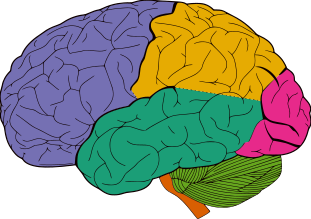
\includegraphics[height=3cm]{dev/wiki/brain_lobes.png}\url{https://en.wikipedia.org/wiki/Frontal_lobe}}
\hspace*{\fill}
\subcaptionbox{\label{fig:nerveFiber}}[.45\textwidth]{
\includegraphics[height=3cm]{dev/wiki/brain_fiber_paths.png}\url{https://en.wikipedia.org/wiki/Association_fiber}}
\hspace*{\fill}
\caption{(a) Illustration of human brain. (b) Illustration of a coronal human brain section. \itodo{a) name brain parts, redo in inkscape}}
\label{fig:human-fiber}
\end{figure}
% 
The frontal, parietal, temporal  and ocipital lobe (see \cref{fig:brainLobes}).
\\
The frontal lobe contains most of the ... functionalities.
The parietal lobe has \dummy{}
The ocipital lobe main function is the signal processing of the visual system.
The temporal lobes contain visual memories as well es auditry functions and language.
\par
The inner part of the brain also include cortival(? -> gm) structures like \dummy{}.
All this structures in the cerebellum and the cerebum contain on thir surfaces (outer as well as inner) a cortical (?) layer, which is filled with cell bodies.
This cells purpase are to process the information of all the signals comming from outside (and inside) the brain.
There are many types of cells involed in this process.
For example some can strengthen a signal or inhibite it.
In the human brain there are several (Billion?) cells which have a high interconnectivity in the local area as well as through the brain to different ...
This high coplex structure is the source of human intelligence, consisnes and much more.
Therefore it is a common goal of humanity to understand the human brain to improve medical treatment as well as \dummy{}.
% 
% \paragraph{Further information}
% This is only a short introduction into the brain architecture.
% It can be further seperated into much more objective parts as well as ...
% This is for example done via cell types and density research like the investigation of cortical layers.
% 
% 
% 
\section{Fiber Architecture} \label{sec:fiberArchitecture}
% 
\begin{figure}[!t]
\centering
\hspace*{\fill}
\tikzset{external/export next=false}
\subcaptionbox{\label{fig:coronalStained}BB 4201: Gray, White Matter, Coronal Section, Stained}[0.6\textwidth]{
\begin{tikzpicture}[]
    \node[inner sep=0pt, anchor = south west] (fig) at (0,0)
    {\includegraphics[width=0.6\textwidth]{dev/brain/BB_4201.png}};
    % \draw[] (0,0) grid (8,5);
    \draw[RED, ultra thick, <-] (5,4) -- ++ (-42:0.75) node[pos=1, anchor=north] {\textbf{WM}};
    \draw[GREEN, ultra thick, <-] (2.4,5) -- ++ (-65:0.75) node[pos=1, anchor=north] {\textbf{GM}};
\end{tikzpicture}
}
\hspace*{\fill}
\subcaptionbox{Cortical layers}[0.3\textwidth]{
\includegraphics[width=0.3\textwidth]{dev/wiki/layers.png}
}
\hspace*{\fill}
% 
\caption[GM, WM, layers]{}
\label{fig:BBrain}
\end{figure}
% 
% 
% 
\begin{figure}[!t]
\centering
% \subcaptionbox{\label{fig:headAndBrain}}[.28\textwidth]{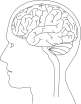
\includegraphics[height=3cm]{gfx/neuroanatomy/human-brain-profile.pdf}}
% \subcaptionbox{}[.42\textwidth]{\includegraphics[height=4cm]{gfx/neuroanatomy/human-brain-section.pdf}}\hfill
% \subcaptionbox{\label{fig:nerveFiber}}[.42\textwidth]{
\includegraphics[angle=90,width=0.75\textwidth,]{gfx/neuroanatomy/neuron-axon_.pdf}
% }
\caption{%(a) Illustration of human brain. 
% (a) Illustration of a coronal human brain section. (b)
Illustration of a neuron with axon and oligodendrocytes. The olegodendrocyte build up a layered lipid structure up, surrounding the axon. The myelin layers are separated along the axon by nodes of Ranvier. \itodo{name parts, ending of axon}}
\label{fig:human-brain}
\end{figure}
% 
Nerve cells are connected via different types of (nerve?) fibers.
A typical nerve cell (see \cref{fig:human-brain}) (if there is such a thing) has a cell body, which processes the incoming information.
The information arrives via dendrites, which are star like tree branches, which will connect to an incoming axon.
The axon is the main (and only) output of the cell.
It travels through the brain to its destination and connects there to a (maybe more or less random) brain cell.
This randomness is also part of the learning process in the brain.
After the brain axons are developed, no new axons are build anymore.
Only the strength of the signals and local structures changes as well as no used connections can be \say{deleted}.
Density of axons \dummy{}.
% Since there are (Billion?) of nerve cells, and there axons need to reach a specific target in a closed volume, the density of nerve fibers is quite high.
There diameter is around $\SI{0.5}{\micro\meter}$ up to several $\si{\micro\meter}$ (see \cref{tag:axonDiameter}).
The axon is surrounded by a myelin sheet, which is a lipid layered structure, build from near by olegodendrides.
These surroundings electric isolates the axon.
This improves the travelling speed of the electric action potential along the axon as well as its signal strength (voltage).
There are many different types of axons.
Some contain a very thick layer of myelin while others have none.
The high density of axons and myelin lets the brain where axons are located, white looking.
Therefore this structure of the brain gets its name \ac{WM}.
The outer cell bodies layer are called \ac{GM}.
In a nissle stained image, where the nerve cells are absorbing light, this is even more visible (see \cref{fig:coronalStained}).
\par
% 
% \begin{figure}[!t]
% 	\centering
% 	\includegraphics{gfx/neuroanatomy/human_wm_after_klinger_dissection.png}
% 	\caption{Electron microscopy image after klinger dissection \cite{destrieux:hal-01261930}. Fiber bundle structures are visible, following the same direction}
% % 	\label{fig:brain_sectioning}
% \end{figure}
% 
\begin{figure}[!t]
	\centering
	\subcaptionbox{}[.49\textwidth]{
	    \includegraphics[width=0.45\textwidth]{dev/brain/auto_seg_axon_0.png}}\hfill
    \subcaptionbox{}[.49\textwidth]{
        \includegraphics[width=0.45\textwidth]{dev/brain/auto_seg_axon_1.png}}
	\caption{Automatic segmentet nerve fiber tissue from an electron microscopy \cite{Abdollahzadeh2019}. }
% 	\label{fig:brain_sectioning}
\end{figure}
% 
Since this \ac{WM} has such a high density of fibers (up to billion in the corpus calosum) it is even under a microscope nearly impossible to investigate single fiber tracts through the brain.
One approach is a myelin staining (see \cref{fig:brainMyelinStain}).
Here nerve fibers which are myelinated are absorbing light (contrast).
Individual nerve fibers can be tracked inside the section.
However already for "smaller" nerve fiber bundles individual nerve fibers are lost.
Especially for dense white matter, no more information can be obtained.
It has also the disadvantage that no 3d orientation information can be easily mapped.
\Cref{fig:brainMyelinStain} shows a section with this technique inside the human thalamus.
It shows different kind of organisations of the nerve fibers.
Nerve fiber bundles are visible (orange) as well as net structures inside the \ac{GM}.
Latter are present to connect the nerve cells with each other inside the \ac{GM}, while the nerve fiber bundles let the axons reach there target area.
\par
% 
\todo{klinger section}
% 
\begin{figure}[!t]
	\centering
	\includegraphics{gfx/neuroanatomy/magic.png}
	\caption{Magic. TPFM auto fluorescence nerve fibers. Origin: \cite{Costantini2020}.}
	\label{fig:brainTPFM}
\end{figure}
% 
\begin{figure}[!t]
	\centering
	\tikzset{external/export next=false}
	\begin{tikzpicture}[]   
     \node[inner sep=0pt, anchor = south west] (fig) at (0,0)
       {\includegraphics[width=\textwidth]{gfx/neuroanatomy/NeuralNet-BrainAtlasDotOrg.png}};
     \draw[Orange, ultra thick] (7.65,6.15) ellipse (1 and 0.5);
     \draw[ProcessBlue, ultra thick] (10,4.5) ellipse (2 and 1);
     \draw[white, ultra thick] (0.5,0.5) -- ++ (0:1) node[pos=0.5, above] {\small $\SI{0}{\micro\meter}$};
    \end{tikzpicture}
% 	\includegraphics[width=\textwidth]{gfx/neuroanatomy/NeuralNet-BrainAtlasDotOrg.png}
	\caption{Myelin Staining. human thalamus, sagital section. \textcolor{Orange}{nerve fiber bundles}. \textcolor{ProcessBlue}{neural net}}
	\label{fig:brainMyelinStain}
\end{figure}
% 
Another tequnique is \ac{TPFM}. 
\cref{fig:brainTPFM} shows a measurement after \ac{3D-PLI} with the \ac{MAGIC} protocol.
This allows fluorescence measurments of the myelin which appears in \ac{3D-PLI} sections after PBS washing \cite{Costantini2021}.
The figure shows the 3d structure of (species, region).
In the lower left part of the volume \ac{WM} is present. 
The border between \ac{WM} and \ac{GM} is in the upper left to the lower right image.
In the upper right corner \ac{GM} is present with individual nerve fibers as well as nerve fiber bundles.
\par
% 
These exemplary data indicate the extreme complexity.
There are a lot more data available.
One comon teqchnique are electorn microscope data.
However the necesarry of a vacuum let the nerve fibers dry out and deform their structure significantly.
\par
% 
For different species with smaller brains, like rodents, imaging techniques like \textit{clearing} have a high potential and could already been used to map an (entire?) brain with axons.
However for a more complex and larger brain, this is up to this point not achieved.
Polarized light imaging, which uses the birefringence property of myelin, is a promising technique, already developed around the 1900, which allows to map the orientation of axons in a brain section.
This technique has, as all microscopic techniques which are using sections, the disadvantage, that the brain has to be cut and measured afterwards.
There are alternative methods like (OCT? \cite{Aumann2019}), which measures the brain section first, and then cuts the upper layer away, and measures the next section afterwards. It uses the reflection of the light than rather the transmitted light through the tissue.
However up to this point no entire large brain like a human brain was measured in its entirety.
Since \ac{3D-PLI} uses the already known sectioning techniques, which are developed since several decades, it can use this knowledge to its advantage.
% 
%
\section{Sectioning}
%
\begin{figure}[!t]
	\centering
    \setlength{\tikzwidth}{0.75\textwidth}
	\inputtikz{gfx/neuroanatomy/brain_sectioning}
	\caption{Illustration of sectioning. a)-b) block with imbedded brain, c) vibrating knife.}
	\label{fig:brain_sectioning}
\end{figure}
% 
For the cutting process, the tissue, \ie{} the brain, has to be frozen and imbedded into a solid material.
One commen material is parafine, however this is not possible for \ac{3D-PLI} \dummy[why?]{}.
For \ac{3D-PLI} it very is important, that the tissue does not build up crystal structures, because these are also birefringence.
Therefore the tissue is first ... into a ... liquid ...
After a time of a few months the tissue will then be frozen into a \SI{-70}{\degree}.
Then the frozen tissue can be fixated with a liquid glue on a cutting plate.
The glue is ...
It is also be used to build up a sourounding fixating material to stabilize the brain in the cutting process.
Additionally markers are fixed which help in the later registration process, which will align the tissue sections in a 3d volume again \cite{Schober2016,Ali2018,Schmitz2018}.
\par
The cutting is done in a microtome (see \cref{fig:brain_sectioning}).
In there the temperature can be held at about \SI{-70}{\degree} and allows no heating of the tissue.
The brain is moved against a vibrating very sharp knife.
This allows for the thin sectioning of about \SI{60}{\micro\meter}.
After the cutting, the tissue is put onto a glass specimen.
Since the tissue is such thin and filigran, it is not always possible to avoid cracks for example.
This also will be as best as possible corrected in the registration process.
The tissue will be ... with a glycerin ... and finally siled with another glass.
To prevent the formation of waves in the tissue, the glass is weighted.
The tissue sections are then stored into a refrigerator at \SI{-70}{\degree\celsius}.
The tissue can then finally be measured in the \ac{3D-PLI} microscopes (see \cref{sec:expSetup} for further techniqule informations).
% 
% 
\section{Axon Literature}
\label{microscopy}
% 
Axon diameter \cite{Liewald2014}:
% 
\begin{table}[!b]
\centering
\pgfplotstabletypeset[
thesisTableStyle,
font=\footnotesize,
col sep=comma,
columns/Name/.style={string type},
columns/Mean/.style={fixed zerofill},
columns/SD/.style={fixed zerofill},
columns/Median/.style={fixed zerofill},
columns/Max/.style={fixed zerofill},
columns/Min/.style={fixed zerofill},
columns/n/.style={dec sep align},
rowbf={1},rowbf={8},rowbf={19},
rowem={2},rowem={5},
rowem={9},rowem={12},rowem={15},
rowem={20},rowem={23},rowem={26},
]{data/axon_distribution.csv}
\caption{axon diameter distribution of the human brain in \si{\micro\meter} \cite{Liewald2014}}
\label{tag:axonDiameter}
\end{table}
% 
\begin{table}[!b]
\centering
\pgfplotstabletypeset[
thesisTableStyle,
font=\footnotesize,
col sep=semicolon,
columns={article,cite,gratio},
columns/article/.style={string type, column name=name, column type = {l}},
columns/cite/.style={string type, column name=cite, column type = {l}},
columns/gratio/.style={string type, column name=$g_{\mathit{ratio}}$},
]{data/gratio.csv}
\caption{human $g_{\mathit{ratio}}$ from invivo mri studies.}
\label{tab:gratio}
\end{table}
% 
axon = 0.5-1.0 diameter (most frequent
thickness of myelin mean = 0.09, median 0.08
-> g-ratio 0.9 (electron microscop, upper boundry)
% 
g-ratio
\cite{Cercignani2017} -> 0.65-0.8 mrt, healty male and female different age, different regions\\
\cite{FitzGibbon2013} -> 0.58-0.84 (Retina), electron microscopy
% 
\itodo{brechungsindex}
% 
% \begin{figure}[!t]
% 	\centering
% 	 \includegraphics[clip, trim=0.65cm 6.25cm 0.4cm 0.5cm]{gfx/neuroanatomy/nature_3d_em_optical_nerve.png}
% 	\caption{\dummy{only show a} Three dimensional electron microscopy reveals changing axonal and myelin morphology along normal and partially injured (*, light green) optic nerves. Origin: \cite{Giacci2018} (reative Commons Attribution 4.0 International License).}
% % 	\label{fig:brain_sectioning}
% \end{figure}
%
\setcounter{chapter}{2}
\chapter{Theory}
\label{sec:theory}
% 
\cleanchapterquote{The first principle is that you must not fool yourself and you are the easiest person to fool.}{Richard P. Feynman}{}%\newline
%
\section{Introduction}
The following section lists the physical theories needed to describe the mathematics behind \ac{3D-PLI}. This includes the basic properties of light with the description of their polarization state, the optical models of the tissue, i.e. the nerve fibers and the mathematical description of the experimental setup of \ac{3D-PLI}. The first part of this chapter was written with the help of \cite{demtroeder2, Fliebach2012}.
% 
% 
% 
\section{Electromagnetic Wave}
% 
Light is an electromagnetic wave. Electromagnetism is first fully described by James Clerk Maxwell. He formulated the Maxwell-Equations \cref{eq::maxwell_general}, generalized from the previous work of Johann Carl Friedrich Gau{\ss}, Michael Faraday and Andr\'{e}-Marie Amp\`{e}re and others. 
% 
% \begin{align} 
% \begin{split} \label{eq::maxwell_macro}
%     \nabla \cdot \vec{D} &= 4\pi\rho_\text{f}\\
%     \nabla \cdot \vec{B} &= 0\\
%     \nabla \times \vec{E} &= -\frac{1}{c} \frac{\partial \vec{B}} {\partial t}\\
%     \nabla \times \vec{H} &= \frac{1}{c} \left(4\pi\vec{J}_\text{f} + \frac{\partial \vec{D}} {\partial t} \right)
% \end{split}
% \end{align}
% 
\begin{align} 
\begin{split} \label{eq::maxwell_general}
    \nabla \cdot \vec{E} &= \frac {\rho} {\varepsilon_0}\\
    \nabla \cdot \vec{B} &= 0\\
    \nabla \times \vec{E} &= -\frac{\partial \vec{B}} {\partial t}\\
    \nabla \times \vec{B} &= \mu_0\left(\vec{j} + \varepsilon_0 \frac{\partial \vec{E}} {\partial t} \right)
\end{split}
\end{align}
% 
with $\nabla \coloneqq \left({\frac{\partial}{\partial x}}, {\frac{\partial}{\partial y}}, {\frac{\partial}{\partial z}} \right)$ as vector differential operator, $\vec{E}$ as eletric field, $\rho$ as electric charge density, $\varepsilon_0$ as permittivity of free space, $\vec{B}$ as magnetic field, $\mu_0$ as permeability of free space and $\vec{j}$ as electric current density.
% 
The first equation states no electric field can be generated without an electric charge (charge conservation).
The second equation states, magnetic monopoles does not exists. The basic entity of an magnetic field is a dipole.
The third and forth equation show the interconnection of the electric and magnetic fields in space and time. A change in the electric field yields to a magnetic field and vice versa. Equation forth additional indicates the creation of a magnetic field from a electric current. The maxwell equation fullfill the continoiut ... $\divergence j + \frac{\partial \rho}{\partial t} = 0$
% 
In a vacuum this simplifies with $\rho = 0$ and $\vec{J} = \vec{0}$ to:
% 
\begin{align}
\begin{split} \label{eq::maxwell_vacuum}
  \nabla \cdot \vec{E} &= 0 \quad\\
  \nabla \cdot \vec{B} &= 0 \quad\\
  \nabla \times \vec{E} &= -\frac{\partial\vec B}{\partial t}\\
  \nabla \times \vec{B} &= \mu_0\varepsilon_0 \frac{\partial\vec E}{\partial t}
  \end{split}
\end{align}
% 
With 
\begin{align}
\begin{split} 
    \nabla \times \nabla \times \vec{E} = -\nabla \times \frac{\partial \vec{B}} {\partial t} &= -\frac{\partial} {\partial t} \left( \nabla \times  \vec{B} \right)\\
    &= -\varepsilon_0 \cdot \mu_0 \frac{\partial^2 \vec{E}}{\partial t^2}
\end{split}
\end{align}
% 
the identity $\nabla \times \left( \nabla \times \vec{A} \right) = \nabla(\nabla \cdot \vec{A}) - \nabla^{2}\vec{A}$ and $\mu_0\varepsilon_0 = \frac{1}{c^2}$, with $c$ as the speed of light\footnote{can be derived from Maxwells equation and Lorentz force in a vacuum}, this further simplifies to:
% 
\begin{align}
\begin{split} \label[pluralequation]{eq::maxwell_wave_equations}
  \frac{1}{c^2} \frac{\partial^2 \vec{E}}{\partial t^2} - \nabla^2 \vec{E} &= 0 \\
  \frac{1}{c^2} \frac{\partial^2 \vec{B}}{\partial t^2} - \nabla^2 \vec{B} &= 0
\end{split}
\end{align}
% 
Another common representation is
% 
\begin{align}
\begin{split} \label{eq::maxwell_wave_equations_box}
  \Box \ \vec{E} &= 0 \\
  \Box \ \vec{B} &= 0
\end{split}
\end{align}
% 
with the help of the d'Alembert operator $\Box \coloneqq \partial^a\partial_a = \nabla^2 - \frac{1}{c^2} \frac{\partial^2}{\partial t^2}$.
% 
This also shows $c^2  \frac{\partial B} {\partial z} = \frac{\partial E}{\partial t} \Rightarrow \vec{E} \cdot \vec{B} = 0$ that the electric and magnetic field components are perpendicular to each other.
% 
\subsection{Solving MW Equ in vacuum}
% 
\Cref{eq::maxwell_wave_equations} have the shape of a wave equation and can therefore as known be solved by
% 
% Using the Maxwell equation in vacuum \ref{eq::maxwell_vacuum}, one can find the most simple solution to the differential equation is a wave:
% 
\begin{align}
\begin{split} \label{eq::dgl_solution}
  \vec{E}( \vec{r}, t ) &= g(\phi( \vec{r}, t )) = g( \omega t - \vec{k} \cdot \vec{r} + \varphi)\\
  \vec{B}( \vec{r}, t ) &= g(\phi( \vec{r}, t )) = g( \omega t - \vec{k} \cdot \vec{r} + \varphi )
\end{split}
\end{align}
% 
where $g$ is any well behaved function and therefore also their superposition.
% 
With the help of
% 
\begin{align}
k = \mathopen| \vec{k} \mathclose| = \frac{\omega}{c} =  \frac{2 \pi}{\lambda}
\end{align}
% 
a planar wave can be descriped by
% 
\begin{align}
\begin{split} \label{eq::plane_wave}
\vec{E}(\vec{r}) &= \vec{E}_0 \cdot e^{ -i \, \vec{k} \cdot \vec{r} }\\
 \vec{B}(\vec{r}) &= \vec{B}_0 \cdot e^{ -i \, \vec{k} \cdot \vec{r} }
\end{split}
\end{align}
% 
% 
% 
\subsection{Polarization}
% 
\begin{figure}[!t]
\centering
\setlength{\tikzwidth}{\textwidth}
\inputtikz{gfx/pli/polarization_state}
\label{fig:polarization_state}
\caption{Illustration of light polarization state.}
\end{figure}
% 
This shows, that the light wave travels in direction of $\vec{k}$ (no it does not, you have to show, that k is perpendicular to E and B).
Therefore the light has a property called polarization.
Polarization is the direction of the, usually, electric field component.
% 
A superposition of x and y wave with z equal to direction of propagation yield to the general form
\begin{align}
\vec{E}(z,t) &= \begin{pmatrix} E_{0x} \cdot e^{ -i \phi_x } \\ E_{0y} \cdot e^{ -i \phi_y } \\ 0 \end{pmatrix}
e^{ -i (kz - \omega t)}
\end{align}
%
\begin{figure}[!t]
\centering
\tikzset{external/export=false}
{
% \captionsetup[sub]{textfont=normalsize}
\captionsetup[sub]{position=top, skip=-14pt}
\tikzset{>=stealth}
\tikzset{cross/.pic={
\draw[->] (-{sqrt(2)},0) -- ({sqrt(2)},0) node[anchor=north]{\footnotesize $E_x$};
\draw[->] (0,-{sqrt(2)}) -- (0,{sqrt(2)}) node[anchor=east]{\footnotesize $E_y$};
}}
% 
\subcaptionbox{}[.3\textwidth]{
\begin{tikzpicture}
\pic at (0,0) {cross};
\draw[] (0, 2) node () {linear, horizontal};
\draw[thick, arrows={Stealth[scale=1]-Stealth[scale=1]}] (-1, 0) -- (1, 0);
\draw[] (0, -2) node () {$\begin{pmatrix} 1&0 \end{pmatrix}$};
\draw[] (0, -3) node () {$\begin{pmatrix} 1&1&0&0 \end{pmatrix}$};
\end{tikzpicture}
}
\subcaptionbox{}[.3\textwidth]{
\begin{tikzpicture}
\pic at (0,0) {cross};
\draw[] (0, 2) node () {linear, vertical};
\draw[thick, arrows={Stealth[scale=1]-Stealth[scale=1]}] (0, -1) -- (0, 1);
\draw[] (0, -2) node () {$\begin{pmatrix} 0&1 \end{pmatrix}$};
\draw[] (0, -3) node () {$\begin{pmatrix} 1&-1&0&0 \end{pmatrix}$};
\end{tikzpicture}
}
\subcaptionbox{}[.3\textwidth]{
\begin{tikzpicture}
\pic at (0,0) {cross};
\draw[] (0, 2) node () {linear, $\pi/4$};
\draw[thick, arrows={Stealth[scale=1]-Stealth[scale=1]}] (-1, -1) -- (1, 1);
\draw[] (0, -2) node () {$\begin{pmatrix} 1&1 \end{pmatrix}$};
\draw[] (0, -3) node () {$\begin{pmatrix} 1&0&1&0 \end{pmatrix}$};
\end{tikzpicture}
}
\\[2em]
\subcaptionbox{}[.3\textwidth]{
\begin{tikzpicture}
\pic at (0,0) {cross};
\draw[] (0, 2) node () {left circular};
\draw[thick] plot[domain=0:360,samples=90,smooth] ({cos(\x)},{sin(\x)});
\draw[thick, arrows={-Stealth[scale=1]}] plot[domain=44:45,samples=1] ({cos(\x)},{sin(\x)});
\draw[thick, arrows={-Stealth[scale=1]}] plot[domain=224:225,samples=1] ({cos(\x)},{sin(\x)});
\draw[] (0, -2) node () {$\begin{pmatrix} 1&i \end{pmatrix}$};
\draw[] (0, -3) node () {$\begin{pmatrix} 1&0&0&-1 \end{pmatrix}$};
\end{tikzpicture}
}
\subcaptionbox{}[.3\textwidth]{
\begin{tikzpicture}
\pic at (0,0) {cross};
\draw[] (0, 2) node () {right circular};
\draw[thick] plot[domain=0:360,samples=90,smooth] ({cos(\x)},{sin(\x)});
\draw[thick, arrows={-Stealth[scale=1]}] plot[domain=46:45,samples=1] ({cos(\x)},{sin(\x)});
\draw[thick, arrows={-Stealth[scale=1]}] plot[domain=226:225,samples=1] ({cos(\x)},{sin(\x)});
\draw[] (0, -2) node () {$\begin{pmatrix} 1&-i \end{pmatrix}$};
\draw[] (0, -3) node () {$\begin{pmatrix} 1&0&0&1 \end{pmatrix}$};
\end{tikzpicture}
}
\subcaptionbox{}[.3\textwidth]{
\begin{tikzpicture}
\pic at (0,0) {cross};
\draw[] (0, 2) node () {unpolarized};
\draw[] (0, -3) node () {$\begin{pmatrix} 1&0&0&0 \end{pmatrix}$};
\end{tikzpicture}
}
}
\caption{polarization states, check vector length,\itodo{test speed}} 
\label{fig:polarization_state_vectors}
\end{figure}
%
\Cref{fig:polarization_state_vectors} shows another representation of the polarization sate of a light wave.
It show the component perpendicular to the travelling direction.
Therefore the time variation can be shown on the xy-plane.
Additionally the states can be describe by the Jones or Stokes calculus, later described in \cref{sec:jones,,sec:mueller_stokes}.
% 
% 
% 
\subsection{Light in medium}
% 
The maxwell equations in ... are described above. They can be solved analog to ... . This yields to some special behavier, \eg{} the magnetic and electic field component get out of phase.
However here only the two properties of absorptiona and difraction are described.
They derivation can be found \eg{} \cite{demtroeder2, Fliebach2012}.
% 
\subsection{Absorption}
% 
\begin{align}
    I = I_0 \exp(-\mu x)
\end{align}
% 
Beersche law of absorption with $\mu = \frac{4\pi \kappa}{\lambda_0}$ where $\kappa$ is the imaginary part of the complex refractive index.
% 
\subsection{Refraction}
% 
\begin{figure}[!t]
\centering
\setlength{\tikzwidth}{\textwidth}
\inputtikz{gfx/pli/refraction}
\label{fig:optic_refraction}
\caption{Illustration of refraction.}
\end{figure}
% 
Refraction is the property of light to change direction as it passes from one medium to another. This can be shown by using the full Maxwell equations  for non-conductive material, \ie{} $\vec{j} = 0, \rho = 0$, that the dgl consit out of a primary wave with from atomic medim induced secundary waves, which leads to a reduction of the velocity of the resulting wave. Mathematically this can be described by a complex number $n = c' / c$.
Using this relationship at a boundary surface between two media, one can show that the incident light beam splits into a reflecting and transmittang light wave. The reflecting light wave has the same angle as the incident light beam relativ the the surface normal. The transmitting light beam however due to the reduction of the velocity, changes its direction described by the snellius ...
\begin{align}
    n_0 \sin \alpha = n_1 \sin \beta
\end{align}

% 
\begin{align}
\underline{n} = n + i\kappa
\end{align}
% 
\begin{align}
\begin{split}
\vec{E}(z, t) &= \operatorname{Re}\! \left[\vec{E}_0 \cdot e^{i\, (kz - \omega t)}\right] \\
&= \operatorname{Re}\! \left[\vec{E}_0 \cdot e^{i\, (2\pi(n + i\kappa)z/\lambda_0 - \omega t)}\right] \\
&= e^{-2\pi \kappa z/\lambda_0} \operatorname{Re}\! \left[\vec{E}_0 \cdot e^{i\, (kz - \omega t)}\right]
\end{split}
\end{align}
% 
% 
% 
\subsection{Birefingence}
%
\begin{figure}[!t]
\centering
\setlength{\tikzwidth}{\textwidth}
\inputtikz{gfx/pli/retardation}
\caption{Illustration of retardation.}
\label{fig:optic_retardation}
\end{figure}
% 
\begin{figure}[!t]
\centering
\subcaptionbox{}[.49\textwidth]{
\setlength{\tikzwidth}{0.49\textwidth}
\inputtikz{gfx/pli/ellipsoid_a}}
\subcaptionbox{}[.49\textwidth]{
\setlength{\tikzwidth}{0.49\textwidth}
\inputtikz{gfx/pli/ellipsoid_b}}
\caption{birefringence elipsoid}
\label{fig:index_elipsoid}
\end{figure}
% 
Material can have a different refractive index depending on the relative orientation and polarization of the light beam.
This property is known as birefringence.
The refractive index can be described as the refractive index $n_o$ and extraordinary  $n_e$.
Since these two are perpendicular to each other, one can split the light beam into the same perpendicular parts and describe each by its own.
These two light beams, except for the trivial case of a light beam is perpendicular to the surfave, have a different direction.
However for small relative length (hängt von n ab, bzw der phasenänderung) the two light beams leave the material at the same point and recombined at the end.
The change of phase is called birefringence and is described by the difference between the .. and ...
% 
\begin{align}
    \Delta n = n_e - n_o \> .
\end{align}
% 
This .. can be visualized by the index ellipsoid \cref{fig:index_elipsoid}.
The change of the amplitude and phase can be described by the following techniques.
% 
% 
% 
\subsection{Jones}
\label{sec:jones}
% 
The Jones calculus, introduced by Robert Clark Jones in 1941, describes the polarization state of a light beam by a complex vector $J$:
% 
\begin{align}
    \vec{J} = \begin{pmatrix} E_x \exp(i \phi_x) \\ E_y \exp(i \phi_y) \end{pmatrix}
\end{align}
% 
The amplitude of the perpendicular components are $E_x$ and $E_y$ with their phase $\phi_x$ and $\phi_y$.
Optical elements, which changes the polarization state, such as a polarization filter and retarder, can be desribed by a matrix:
% 
\begin{align}
\begin{split}
\mat{P}_x = 
\begin{pmatrix}
1 & 0 \\ 0 & 0
\end{pmatrix}
, \,
\mat{P}_y = 
\begin{pmatrix}
0 & 0 \\ 0 & 1
\end{pmatrix}
, \,
\mat{M} =
\begin{pmatrix}
e^{i \varphi_x} & 0 \\ 0 & e^{i \varphi_y}
\end{pmatrix}
, \,
\Lambda_{1/4}=
e^{\frac{i \pi}{4}}
\begin{pmatrix}
1 & 0 \\ 0 & -i
\end{pmatrix}
\end{split}
\end{align}
% 
A rotation of the axis can be achieved by a 2d rotation matrix $\mat{R}$:
% 
\begin{align}
\begin{split}
\mat{M}(\theta )=\mat{R}(\theta )\cdot\mat{M}\cdot\mat{R}(-\theta )
, \>
\mat{R}(\theta ) = 
\begin{pmatrix}
\cos \theta & -\sin \theta \\
\sin \theta & \cos \theta
\end{pmatrix}
\end{split}
\end{align}
% 
% 
% 
\subsection{M\"uller-Stokes}\label{sec:Mueller-Stokes}
\label{sec:mueller_stokes}
% 
Analog to \cref{sec:jones} the M\"uller-Stokes formalism, described by George Gabriel Stokes in 1852, also describes the polarication state of a light beam.
However it does not use the absolute .. but the relative polarication between both components:
% 
\paragraph{Stokes vector}
\begin{align}
\begin{split}
S_0 &= I \\
S_1 &= I p \cos 2\psi \cos 2\chi \\
S_2 &= I p \sin 2\psi \cos 2\chi \\
S_3 &= I p \sin 2\chi
\end{split} \hspace{-6em}
\begin{split}
& \equiv \langle E_x^{2} \rangle + \langle E_y^{2} \rangle \\
%  & = \langle E_a^{2} \rangle + \langle E_b^{2} \rangle \\
%  & =  \langle E_l^{2} \rangle + \langle E_r^{2} \rangle \\
& \equiv \langle E_x^{2} \rangle - \langle E_y^{2} \rangle \\
& \equiv \langle E_a^{2} \rangle - \langle E_b^{2} \rangle \\
& \equiv  \langle E_l^{2} \rangle - \langle E_r^{2} \rangle
\end{split}
, \,
\vec{S} =
\begin{pmatrix} S_0 \\ S_1 \\ S_2 \\ S_3\end{pmatrix}
\end{align}
% 
% \begin{align}
% \begin{split}
% S_0 & \equiv \langle E_x^{2} \rangle + \langle E_y^{2} \rangle \\
%  & = \langle E_a^{2} \rangle + \langle E_b^{2} \rangle \\
%  & =  \langle E_l^{2} \rangle + \langle E_r^{2} \rangle \\
% S_1 & \equiv \langle E_x^{2} \rangle - \langle E_y^{2} \rangle \\
% S_2 & \equiv \langle E_a^{2} \rangle - \langle E_b^{2} \rangle \\
% S_3 & \equiv  \langle E_l^{2} \rangle - \langle E_r^{2} \rangle
% \end{split}
% \end{align}
% 
Therefore the phase can not be described anymore.
However the relative phase information is stored and can be used to describe also polarization states of polarization filters, which can not be described by Jones.
Aanlog to Jones one can formulate the matrices for the optical components:
% 
\paragraph{Linear Polarizer}
\begin{align}
\mat{P}_x=\frac{1}{2}
\begin{pmatrix}
    1 & 1 & 0 & 0 \\
    1 & 1 & 0 & 0 \\
    0 & 0 & 0 & 0 \\
    0 & 0 & 0 & 0
  \end{pmatrix}
, \,
\mat{P}_y=\frac{1}{2}
\begin{pmatrix}
     1 & -1 & 0 & 0 \\
    -1 &  1 & 0 & 0 \\
     0 &  0 & 0 & 0 \\
     0 &  0 & 0 & 0
\end{pmatrix}
\end{align}
% 
\paragraph{retarder}
\begin{align}
\mat{M}=\
\begin{pmatrix}
    1 & 0 & 0 &  0 \\
    0 & 1 & 0 &  0 \\
    0 & 0 & \cos \delta & \sin \delta \\
    0 & 0 & -\sin \delta &  \cos \delta
\end{pmatrix}
\end{align}
% 
\paragraph{Quarter-wave plate (fast-axis vertical)}
\begin{align}
\Lambda_{1/4}=\
\begin{pmatrix}
    1 & 0 & 0 &  0 \\
    0 & 1 & 0 &  0 \\
    0 & 0 & 0 & -1 \\
    0 & 0 & 1 &  0
\end{pmatrix}
\end{align}
% 
\paragraph{Rotation Matrix}
\begin{align}
\mat{R}(\theta)=
\begin{split}
\begin{pmatrix}
    1 &                0 &               0 & 0 \\
    0 & \cos{(2\theta)} & -\sin{(2\theta)} & 0 \\
    0 & \sin{(2\theta)} & \cos{(2\theta)} & 0 \\
    0 &                0 &               0 & 1
  \end{pmatrix}
\end{split}
\end{align}
% 
% \paragraph{Rotation Matrix}
% \begin{align}
% \frac{1}{2}
% \begin{pmatrix}
%     1 &                0 &               0 & 0 \\
%     0 &  \cos{(2\theta)} & \sin{(2\theta)} & 0 \\
%     0 & -\sin{(2\theta)} & \cos{(2\theta)} & 0 \\
%     0 &                0 &               0 & 1
% \end{pmatrix}
% \end{align}
\todo{matrix multi}
% 
% \section{Tissue Discretization}
% % 
% By deviding the volume into small diskreticed subvolumes, one can multiply the .. all together and ... (analog Riemann sum)
% \begin{align}
%     \int F \, dt \approx \sum_n F \, \Delta t
% \end{align}
% see simulation?
% 
%  see simulation
% \paragraph{Micro vs Macro:}
% % 
% % \begin{align}
% %   \int_{y_\textit{min}}^{y_\textit{max}} \vec{v}(y) \,dy\\
% %   x = const
% %   y = y(\alpha,x) = tan(\alpha) \cdot x\\
% %   \vec{v}_r = \begin{pmatrix} \cos(\alpha)\\ \sin(\alpha)\\0\end{pmatrix}, \, \vec{v}_p = \begin{pmatrix} 0\\ 0\\1\end{pmatrix}\\
% %   \vec{v}_r = \begin{pmatrix} \cos(\arctan(y/x))\\ \sin(\arctan(y/x))\\0\end{pmatrix}\\
% %   \int_{y_\textit{min}}^{y_\textit{max}} \vec{v}_p(y) \,dy = (y_\textit{max} - y_\textit{min}) \cdot e_z\\
% %   \int_{y_\textit{min}}^{y_\textit{max}} \vec{v}_r(y) \,dy = \int_{y_\textit{min}}^{y_\textit{max}} \cos(\arctan(y/x)) dy \cdot e_x \\
% %   = x\left(\sinh^{-1}(y_\textit{max}/x) - \sinh^{-1}(y_\textit{min}/x)\right) \\
% %   = 2x \left(\sinh^{-1}\left(\frac{2\sqrt{R-x^2}}{x}\right)\right)
% % \end{align}
% % 
% % \begin{align}
% %     % \frac{\oint \vec{v}_z \mathrm{d}A}{\oint \vec{v}_x \mathrm{d}A} = 
% %     % \frac{\int_{-1}^{1}\abs{\vec{v}} \mathrm{d}x}{\int_{-\frac{\pi}{2}}^{\frac{\pi}{2}} \abs{\vec{v}} \cos(\varphi) \mathrm{d}\varphi} =
% %     % \frac{2}{1}
% %     \frac{A_{\Box}}{A_{\circ}} = \frac{4}{\pi}
% % \end{align}
% % 
% \todo{why 2*dn?}
% 
\section{Experimental Setup}\label{sec:expSetup}
%
\begin{figure}[!t]
    \captionsetup[sub]{position=top}
    \setlength{\tikzwidth}{\textwidth}
	\centering
	\subcaptionbox{\label{setup-lap} \ac{LAP}}[\textwidth]{
% 		\resizebox{0.95\textwidth}{!}{
		\inputtikz{gfx/pli/pli_setup}
% 	}
	}\\
	\subcaptionbox{\label{setup-pm} \ac{PM}}[\textwidth]{
% 		\resizebox{0.95\textwidth}{!}{
		\inputtikz{gfx/pli/pli_setup_pm}
% 	}
	}
	\caption{Illustration of PLI setup.}
	\label{fig:pli_setup}
\end{figure}
%
\begin{figure}[!t]
    % \captionsetup[sub]{position=top}
    \setlength{\tikzwidth}{0.3\textwidth}
	\centering
	\subcaptionbox{\ac{LAP}}[.49\textwidth]{
			\inputtikz{gfx/pli/pli_detail}}\hfill
	\subcaptionbox{\ac{PM}}[.49\textwidth]{
			\inputtikz{gfx/pli/pli_detail_pm}}
	\caption{Illustration of detail PLI setup.}
	\label{fig:pli_detail}
\end{figure}
%
The \ac{3D-PLI} setup is described in \cite{Axer2011} with the tiltable light beam microscope (LMP) in \cite{Wiese:887678}.
For the routine measurements two (three) microscope systems are currently in use.
The first use of a high throughput microscope is the \ac{LAP} with a pixel size of about \SI{60}{\micro\meter}. \footnote{can be change by the optic also to $\SI{40}{\micro\meter}$ and $\SI{20}{\micro\meter}$, but remains for the routine measurements with $\SI{60}{\micro\meter}$.}
It consist out of a led light source (\SI{525}{\nano\meter}), a rotatable polarization filter, a rotatable quarter wave retarder, the specimen stage, which can be tilted for oblique views, a rotatable polarizer.
Both polarizer and quarter wave retarder are rotated at the same time.
The both polarizers have a phase offset of $\SI{90}{\degree}$, the first polarizer and the quarter wave retarder of $\SI{45}{\degree}$ (see (see \cref{setup-lap}).
The second system \ac{LMP3D} microscope fullfills the same measurments, however the retarder is placed after the tissue specimen and fixed with the polarizer without any rotations (see \cref{setup-pm}).
Mathematically it measures the same signal.
\footnote{The rotatable filters of the \ac{LAP} has the advantage, that noise like dust particles can be easy identified and removed. Since the microscop is in a more confined "box" this is not necesarry.}
A difference is that the optical path is in reverse to the \ac{LAP} system.
Since there is a mirror in the path, the image is flipped again so that the coordinate systems stays the same (see \cref{fig:pli_detail}).
% 
\subsection{Signal}
% 
From the M\"{u}ller Matrices (\cref{sec:Mueller-Stokes}) as shown in \cite{MenzelMaster,MenzelDissertation}, that the intensity signal, measured by the \ac{CCD}-sensor, follows a sinusiodal curve:
% 
% \begin{align}
% I = \underbrace{\frac{I_0}{2}}_{\mathclap{\mathit{transmittance}}}
%     \bigl[ \sin\bigl(2\rho - 2{\underbrace{\vphantom{\frac{I_0}{2}} \varphi}_{\mathclap{\mathit{direction}}}} \bigr)
%     \cdot \sin \bigl( {\underbrace{\vphantom{\frac{I_0}{2}} 2\pi\frac{d \dn}{\lambda} \cos^2\left( \alpha \right)}_{\mathclap{\delta \, \coloneqq \, \mathit{retardation}}}} \bigr) \bigr]
% \end{align}
\begin{align}
\label{eq:pli_signal}
\begin{split}
I =\frac{I_0}{2}\bigl[ \sin\bigl(2\rho - 2\varphi \bigr)\cdot \sin \bigl( 2\pi\frac{d \dn}{\lambda} \cos^2\left( \alpha \right) \bigr) \bigr] \\
\text{with} \enspace \delta \coloneqq 2\pi\frac{d \dn}{\lambda} \cos^2\left( \alpha \right) \enspace 
\text{and} \enspace \trel \coloneqq \frac{d \dn}{\lambda}
\end{split}
\end{align}
% 
Since \cref{eq:pli_signal} describes a sinosoidal signal, the fourier analysis is a obvious choise.
For a discrete, aquidistant measurement of the rotation angles $\rho$, one can use the fourier series with the three coefficients to describe the signal:
% 
% \begin{align}
% \begin{split}
% A \sin(\omega t + \alpha) + B \sin(\omega t + \beta) &= \sqrt{C^2 + D^2} \cdot \sin \, \left( \omega t + \tan^{-1} \left( \frac{D}{C} \right) \right)
% \end{split}
% \\
% \begin{split}
% C &= A \cos(\alpha)+ B \cos(\beta)\\
% D &= A \sin(\alpha)+ B \sin(\beta)
% \end{split} \nonumber 
% \end{align}

\begin{align}
\begin{split}
\rho &= [\SI{0}{\degree}, \frac{1\cdot180}{N+1}\si{\degree}, \frac{2\cdot180}{N+1}\si{\degree}, ..., \frac{N\cdot180}{N+1}\si{\degree}]\\
a_0 &= \frac{1}{N} \sum(\mathit{data})\\
a_1 &= \frac{2}{N} \sum(\mathit{data} \cdot \sin(2 \cdot \rho)\\
b_1 &= \frac{2}{N} \sum(\mathit{data} \cdot \cos(2 \cdot \rho)
\end{split}
\end{align}

With these the final \ac{3D-PLI} modalities are calculated:

\begin{align}
\begin{split}
\mathit{transmittance} &= 2 \cdot a_0\\
\mathit{direction} &= 0.5 \cdot \atantwo(-b_1 / a_1)\\
\mathit{retardation} &= \frac{\sqrt{a_1^2 + b_1^2}}{a_0}
\end{split}
\end{align}



% 
\subsection{Tilted signal}
% 
To be able to analyse the inclination $\alpha$ one has to distiguish the relative strength of the birefringence from the $\cos^2(\alpha)$.
For this purpose a tiltable specimen was developed, which allows measuring the light signal through the tissue with a different angle of incidenc.
This mean, that tissue and therefore the nerve fibers also change their orientation by the tilting angles $\theta, \varphi$.
Additionally the distance the light travels through the tissue, elongigates by $1/\cos(\theta)$ \cref{fig:tilted_side_view}.
% 
Depending on the \pixelsize{}, in the case of the \ac{LAP} system, this light travels though the same volume, but with another orientation.
Therefore a measurement of multiple light paths can be ... and the resulting signals can be used to analyse the inclination and relative birefrigente tissue thickness \trel{}.
In the case of a tiltible specimen, the angle of incidence on the glass ... and the tissue also changes the angle of the light by snellius law.
All angles mentiont here are if not specified always the change of angle of the light inside the tissue (see \cref{fig:tilting_camera_view}). 
This also leads to a perspective shift, which has to be corrected by a registration process.
In this case an affine transformation.
% 
In \cite{Schmitz2018} this analys published under the name of \ac{ROFL}, which builds up on the work of \cite{Wiese:887678}.
The idea is to fit the measured signals of all light paths simultaniously.
Because the change of signal is proportional to the $\cos(\alpha)$ this however means, that for steep fibers, the changes are not only small, but also the amplitude of the signal is very small.
This leads to the problem of increasing uncertanty with increasing inclination angle.
\\
A further problem is that for a smaller \pixelsize{} the light path cannot be neglected anymore.
For the \ac{LMP3D} system this means, that with a maximal tilting angle of about $\SI{3}{\degree}$ and a usually tissue thickness of $\SI{60}{\micro\meter}$ the light path is measured in n pixels away from the non tilting case, if the rotation point is in the center of the tissue.
\\
However for homoginoius tissue, like the \ac{WM} may be some regions, the analysis technique can still be applied.
A change in density, orientation or dispersion however will lead to a false result.
% 
% 
% 
\section{Orientation}
% 
\begin{figure}[!t]
\centering
\setlength{\tikzwidth}{0.4\textwidth}
\begin{center}
\begin{tabular}{m{6cm}m{6cm}}
\includegraphics[width=\tikzwidth]{gfx/pli/color_sphere.png}
&
\inputtikz{gfx/pli/hsv_sphere}
\\
\begin{minipage}[t]{0.42\textwidth}
\leavevmode\subcaption{2d hsv sphere}
\end{minipage}
&
\begin{minipage}[t]{0.42\textwidth}
\leavevmode\subcaption{\label{fig:sphere}3d hsv sphere}
\end{minipage}
\end{tabular}
\end{center}
% 
\vspace{-1em} % because of tabular?
\caption{collor spheres}
\label{fig:spheres}
\end{figure}
% 
% 
The orientation of the birefringence axis is descibed by the direction angle $\varphi$ and inclination angle $\alpha$ (see \cref{fig:sphere}).
To be able to show a 3d information, the \textit{hsv-black} is usually shown in \ac{3D-PLI}.
It color code the orientation by:
\begin{align}
\begin{split}
    H &= \varphi/\pi\\
    S &= 1\\
    V &= 1-\alpha / \pi/2
\end{split}
\end{align}
This way the color corresponds to the direction, and the color value to the inclination.
Since the orientation, unlike a vector, covers only a half sphere, the colors are point symmetric.
% 
% fig:spheres
% 
% 
\section{optical resolution}
\label{sec:opticalResolution}
% 
The optical resolution of an imaging system describes the minimal size of on object which can still be resolved.
This property is limited by aberration and diffraction which both cause a blurring of the resulting image.
Ernst Abbe described as on of the first that the resulition corrlates with the lightwave $\lambda$: 
\begin{align}
d=\frac{ \lambda}{2 n \sin \theta} = \frac{\lambda}{2\mathrm{NA}} \> .
\end{align}
$d$ is the minimal resolvable distance, $n$ the refractive index, $\theta$ the angle of a spot light, which can be combined to the better known numerical aperture $\mathrm{NA}$.
This results in an absolute threshold for a light microscope above which the resolution can no longer be improved.
For the wavelength used in \ac{3D-PLI} with $\lambda = \SI{525}{\nano\meter}$ and a numerical apperatur of $\mathrm{NA} = \SI{}{}$ this yields to a limit of \dummy{}.
% 
\begin{figure}[!t]
\setlength{\tikzwidth}{0.45\textwidth}
\centering
% \subcaptionbox{}{
\inputtikz{gfx/pli/rayleigh}
\caption[Raylay criterium]{rayleigh criteria. The minima of the one function is in the maxima of the other.}
\label{fig:rayleigh}
\end{figure}
% 
\cleardoublepage
\setcounter{chapter}{3}
\chapter{3D Polarized Light Imaging}
\label{sec:pli}
%
\section{Introduction}
% 
This chapter gives an overview of \ac{3D-PLI}.
First, the necessary preparation of the brain tissue is described, including its cutting process and the subsequent mounting.
The second part describes the \ac{3D-PLI} microscopic technique, which allows measuring the orientation of the optical axis that corresponds to the orientation of the myelinated nerve fibers.
The foundation of the measured \ac{3D-PLI} signal and the optical limits in microscopy are described as a basis for the simulation in the following chapters. 
% 
% 
% 
\section{Brain Tissue Preparation and Sectioning}
% 
After the organism death, the brain is removed from the skull within $\SI{24}{\hour}$.
In order to prevent the further degeneration of the brain tissue, it is immersed in a solution of $\SI{4}{\percent}$ formaldehyde and $\SI{20}{\percent}$ glycerin for several days.
Then it is frozen at $\SI{-80}{\celsius}$ as preparation for sectioning.
Then the tissue is fixated with liquid glue on a plate, which allows to place it within a microtome.
The microtome consists of a chamber cooled at about $\SI{-70}{\celsius}$.
A vibrating knife is used to section the brain into $\SI{60}{\micro\meter}$ sections (see \cref{fig:brain_sectioning}).
After each cut, the sections are manually placed onto a glass specimen, surrounded by glycerin and covered with a thin optical glass (see \cref{fig:brain_section}).
To preserve the sections for the microscopic measurement, they are placed in a freezer at approximately $\SI{-70}{\celsius}$.
The \ac{3D-PLI} measurement takes place at room temperature. \cite{Axer2011}
% 
\begin{figure}[!t]
	\centering
    \setlength{\tikzwidth}{0.475\textwidth}
    \subcaptionbox{%
        \label{fig:brain_sectioning}
        Illustration of the sectioning process. The brain is fixed with glue to stabilize it for the cutting process. A microtome is used to cut the tissue by using a vibrating diamond blade over which the tissue block is moved.
    }[\tikzwidth]{\inputtikz{gfx/neuroanatomy/brain_sectioning}}
    \hfill
    \subcaptionbox{%
        \label{fig:brain_section}
        A section is placed on a glass specimen, to protect it from environmental influences. It is covered with a second, thinner glass plate, which is sealed with nail polish.
    }[\tikzwidth]{\inputtikz{gfx/neuroanatomy/brain_section}}
	\caption{Brain sectioning and sealing illustration.}
\end{figure}
% 
% 
% 
\section{Experimental Setup}\label{sec:expSetup}
%
In \ac{INM-1}, there exist three microscopic setups based on identic physical principles \cite{Axer2011} (see \cref{fig:pli_setup}).
Polarized light with a wavelength of about $\SI{525}{\nano\meter}$ is irradiated through the tissue section. \footnote{The exact wavelength depends on the microscope.}
A rotatable polarizer is mounted in front of the tissue in the beam path, and a fixed circular polarizer is mounted behind the tissue.
By rotating the polarizer, the change in intensity is measured with a \ac{CCD}-sensor.
\par
% 
The first experimental setup is called \ac{LAP}.
It is used to measure an entire brain section at a resolution of $\SI{60}{\micro\meter}$. \footnote{It is also possible to aquire images with a pixel size of $\approx \SI{40}{\micro\meter}$ and $\approx \SI{20}{\micro\meter}$ by changing the focal length.}
\par
% 
The \ac{LMP} microscope allows measuring a tile of $\num{2048}\times\num{2048}$ pixels with a pixel size of $\SI{1.3}{\micro\meter}$.
By measuring the tissue with multiple overlapping images, the overlapping tiles can be combined into an overall image with a stitching algorithm. 
This setup is not able to change the light path.
The 3D information can be estimated by analyzing the distribution of retardation and transmittance, however, the inclination sign cannot be detected.
\par
% 
\begin{figure}[!t]
    \captionsetup[sub]{position=top}
    \setlength{\tikzwidth}{\textwidth}
	\centering
    \inputtikz{gfx/pli/pli_setup_pm}
	\caption{Illustration of \acs{3D-PLI} setup.}
	\label{fig:pli_setup}
\end{figure}
% 
The third setup is the \ac{LMP3D} microscope \cite{Wiese:887678}.
By using a conical light path and a slit, only light of a particular angle can pass and therefore through the tissue.
By changing the position of the slit, different light paths can be applied with a maximal tilt angle of $\SI{3.9}{\degree}$.
\par
% 
The tilted light beam in the \acs{LAP} and the \acs{LMP3D} are measured at four perpendicular orientations: North, East, South and West.
\par
%
The final image is captured by a camera that uses a \ac{CCD} sensor, consisting of an array of \ac{MOS} capacitors.
Each capacitor stores an electric charge that is released by incident photons using the photoelectric effect.
After a readout process, which also includes electrical amplification, the resulting values can be stored as an image.
Its value, as long as the capacitors are not saturated or the amplification does not exceed its limits, is linearly correlated with the number of photons.
The signal, however, is affected by noise which comes mainly from two parts.
First is the thermal noise that can lead to electrical charges in the \ac{MOS} capacitors. 
Second, the amplification of the signal underlies a noise usually from a non-ideal direct current and non-ideal electric components like transistors, which is needed for the amplification process.
These noise sources combine to produce a Poisson-like distribution due to the nature of digital positive values produced by the analog-to-digital converter.
A normal distribution can model the intensity values $\gg 0$.
%
%
%
\section{Intensity Signal}\label{sec::intSignal}
%
From the M{\"u}ller-Stokes matrices (\cref{sec:MuellerStokes}), the intensity signal, which is the first component of the Stokes vector, follows a sinusoidal curve \cite{MenzelMaster,MenzelDissertation}:
%
\begin{align}
\label[pluralequation]{eq:pli_signal}
\centering
\begin{gathered}
I(\rho, \varphi, \alpha, d) =\frac{I_0}{2}\left[ 1+ \sin\left(2\rho - 2\varphi \right)\cdot \sin \left( 2\pi\frac{d \dn}{\lambda} \cos^2\left( \alpha \right) \right) \right] \\
\text{with} \enspace \delta \coloneqq 2\pi\frac{d \dn}{\lambda} \cos^2\left( \alpha \right) \enspace
\text{and} \enspace \trel \coloneqq 4 \frac{d \dn}{\lambda}
\end{gathered}
\end{align}
%
\Cref{eq:pli_signal} describes a sinusoidal signal.
For a discrete, equidistant measurement of the rotation angles $\rho$, one can use the Fourier series with the first three coefficients to describe the signal:
%
\begin{align}
\begin{split}
\rho &= \left[0, \frac{\pi}{N+1}, \frac{2\pi}{N+1}, ..., \frac{N\pi}{N+1}\right]\\
a_0 &= \frac{1}{N} \sum_i^N I_i\\
a_1 &= \frac{2}{N} \sum_i^N I_i \cdot \sin(2 \rho_i)\\
b_1 &= \frac{2}{N} \sum_i^N I_i \cdot \cos(2 \rho_i)
\end{split}
\end{align}
%
The current routine measurements take $N=\SI{9}{}$ images.
These are used to calculate the final \ac{3D-PLI} modalities (see \cref{fig:vervetpli}):
%
\begin{figure}[!t]
\setlength{\tabcolsep}{0pt}
\setlength{\tikzwidth}{0.43\textwidth}
\tikzset{external/export=false}
\begin{tabular}{cc}
% 
\begin{tikzpicture}[baseline, trim axis left, trim axis right]
\begin{axis}[
width=\tikzwidth,
axis equal image,
enlargelimits=false,
scale only axis,
point meta min=6851,point meta max=13703,
% xmin=0,xmax=947,ymin=0,ymax=727,
hide axis,
colorbar horizontal,colormap/cividis,
colorbar style={%
    every x tick label/.append style={font=\footnotesize},
    xtick={6851,13703},
    xticklabels={0,$I_{\mathit{max}}/2$},
    scaled x ticks=false,
    }
]
\addplot [forget plot] graphics [
xmin=0,xmax=947,ymin=0,ymax=727,
] {gfx/vervet1818/Vervet1818_60mu_70ms_s0550_a00_d000_Transmittance_6851_13703_.png};
\end{axis}
\end{tikzpicture}
&
\begin{tikzpicture}[baseline, trim axis left, trim axis right]
\begin{axis}[
width=\tikzwidth,
axis equal image,
enlargelimits=false,
scale only axis,
point meta min=0,point meta max=180,
% xmin=0,xmax=947,ymin=0,ymax=727,
hide axis,colorbar horizontal,colormap/twilight,
colorbar style={%
    every x tick label/.append style={font=\footnotesize},
    xtick={0,90,180},
    xticklabels={$\SI{0}{\degree}$,$\SI{90}{\degree}$,$\SI{180}{\degree}$},
    }]
\addplot [forget plot] graphics [
xmin=0,xmax=947,ymin=0,ymax=727,
] {gfx/vervet1818/Vervet1818_60mu_70ms_s0550_a00_d000_Direction_0_180_.png};
\end{axis}
\end{tikzpicture}
\\[-1.5ex]
% 
\multicolumn{1}{l}{
\begin{minipage}{0.5\textwidth}
\leavevmode\subcaption{transmittance}
\end{minipage}}
&
\multicolumn{1}{l}{
\begin{minipage}{0.5\textwidth}
\leavevmode\subcaption{direction}
\end{minipage}}
\\[1.5em]
% 
\begin{tikzpicture}[baseline, trim axis left, trim axis right]
\begin{axis}[
width=\tikzwidth,
axis equal image,
enlargelimits=false,
scale only axis,
point meta min=0,point meta max=0.858,
% xmin=0,xmax=947,ymin=0,ymax=727,
hide axis,colorbar horizontal,colormap/cividis,
colorbar style={%
    every x tick label/.append style={font=\footnotesize},}]
\addplot [forget plot] graphics [
xmin=0,xmax=947,ymin=0,ymax=727,
] {gfx/vervet1818/Vervet1818_60mu_70ms_s0550_a00_d000_Retardation_0_0858_.png};
\end{axis}
\end{tikzpicture}
&
\begin{tikzpicture}[baseline, trim axis left, trim axis right]
\begin{axis}[
width=\tikzwidth,
axis equal image,
enlargelimits=false,
scale only axis,
% xmin=0,xmax=947,ymin=0,ymax=727,
hide axis,
]
\addplot graphics [
xmin=0,xmax=947,ymin=0,ymax=727,
] {gfx/vervet1818/Vervet1818_60mu_70ms_s0550_a00_d000_FOM_HSVBlack.png};
\addplot [forget plot] graphics [
xmin=0,xmax=125,ymin=602,ymax=727,
] {gfx/pli/color_sphere.png};
\end{axis}
\end{tikzpicture}
\\
% 
\multicolumn{1}{l}{
\begin{minipage}{0.5\textwidth}
\leavevmode\subcaption{retardation}
\end{minipage}}
&
\multicolumn{1}{l}{
\begin{minipage}{0.5\textwidth}
\leavevmode\subcaption{\label{fig:exampleFom}fiber orientation map (FOM)}
\end{minipage}}
\end{tabular}

\caption[3D-PLI modalities]{3D-PLI modalities for a coronal section of a vervet monkey brain.}
\label{fig:vervetpli}
\end{figure}
%
\begin{align}
\begin{split}
\mathit{transmittance} &\coloneqq 2 \cdot a_0 \vphantom{I_0/2} \\
\mathit{direction} &\coloneqq 0.5 \cdot \atantwo(-b_1 / a_1) \vphantom{\varphi} \\
\mathit{retardation} &\coloneqq \frac{\sqrt{a_1^2 + b_1^2}}{a_0}  \vphantom{\sin(\delta)}
\end{split}
\hspace{-7em}
\begin{split}
& \mathrel{\widehat{=}} I_0/2 \vphantom{2 \cdot a_0}\\
& \mathrel{\widehat{=}} \varphi \vphantom{0.5 \cdot \atantwo(-b_1 / a_1)} \\
& \mathrel{\widehat{=}} |\sin(\delta)| \vphantom{\frac{\sqrt{a_1^2 + b_1^2}}{a_0}}
\end{split}
\end{align}
%
The \textit{transmittance} describes the tissue light transmittance, \ie{}, how much light passes through the tissue.
The \textit{direction} describes the signal phase, corresponding to the direction of the macroscopic optical axis and therefore the direction of the nerve fibers.
The \textit{retardation} corresponds to the amplitude of the signal, \ie{}, the strength of the retardation.
%
%
\section{Tilting Analysis} \label{sec::InclAnalysis}
%
To analyze the optical axis inclination $\alpha$, one has to distinguish the relative strength of the birefringence from the term $\cos^2(\alpha)$.
For this purpose, the tissue is tilted allowing the light signal to be measured through the tissue at a different angle of incidence \cite{Axer2011, Wiese:887678} (see \cref{sec:expSetup}).
Therefore, the tissue and its underlying nerve fibers change their orientation due to the tilt angles $\theta$ and $\varphi$.
In addition, the distance the light travels through the tissue increases by $1/\cos(\theta)$ (see \cref{fig:tilted_side_view}).
\par
%
Depending on the \Pixelsize{}, light passes through the same volume but with a different orientation.
Therefore, multiple light paths can be measured, and the resulting signals can be used to analyze the inclination $\alpha$ and relative birefringence tissue thickness \trel{}.
The angle of incidence of the light changes the path of the light by Snell's law \cref{eq:Snellius}.
Which results in a perspective shift that a registration process must correct.
However, this effect can be neglected in the simulation, since it only adds a parallel offset.
\par
%
An algorithm was developed under the name \ac{ROFL} to analyze the tilting signal \cite{Wiese:887678,Schmitz2018}.
The idea is to fit the measured signals of all light paths simultaneously.
Since the change in the signal is proportional to $\cos(\alpha)$, for steep fibers, both the changes of $\frac{\partial}{\partial \alpha} \cos(\alpha)$ and the amplitude of the signal are very small, which leads to the problem of increasing uncertainty while the inclination angle increases.
\par
%
Another difficulty is that for a smaller \Pixelsize{}, the light path can no longer be neglected.
For the \ac{LMP3D}-system (with a tilt angle of $\SI{3.9}{\degree}$ and a tissue thickness of $\SI{60}{\micro\meter}$), the tilted light path is measured about $\SI{4}{\pixel}$ away from the non-tilting measurement.
This means that other parts of the tissue affect the light from the different tilt views.
This effect can be neglected for homogeneous tissue regions, such as parts in the dense \ac{WM}.
However, for single fiber paths, such as visible in the \ac{GM} or complicated paths like in crossing the effect on th inclination analysis is an open question.
%
%
%
\section{Optical Resolution}
\label{sec:opticalResolution}
%
The optical resolution of an imaging system describes the minimum size of an object that can still be resolved.
This property is limited by aberration and diffraction.
Aberration causes blurring of the image, while diffraction can lead to superimposed diffraction patterns.
If diffraction is caused by many small objects in relation to the resolution, this also looks like blurring.
\par
%
Ernst Abbe was one of the first to describe that the resolution correlates with the light wave $\lambda$:
\begin{align}
d=\frac{ \lambda}{2 n \sin \theta} = \frac{\lambda}{2\mathrm{NA}} 
\end{align}
$d$ is the minimum resolvable distance, $n$ the refractive index, $\theta$ the angle of a light spot, which can be combined to the better known numerical aperture $\mathrm{NA}$.
A more common definition is the Rayleigh limit given by
\begin{align}
d=1.22\frac{\lambda}{2\mathrm{NA}} \, ,
\end{align}
where $d$ is the distance between two light spots, where the first intensity maxima of the first slit is on the first minima of the second slit (see dashed line \cref{fig:rayleigh}).
The wavelength used in \ac{3D-PLI} is $\lambda = \SI{525}{\nano\meter}$ and a numerical aperture of $\mathrm{NA} \approx \SI{0.15}{}$, which results in a limit of about $\SI{2.1}{\micro\meter}$ \cite{MenzelDissertation}.
%
\begin{figure}[!t]
\setlength{\tikzwidth}{0.5\textwidth}
\centering
% \subcaptionbox{}{
% \tikzset{external/force remake=true}
\inputtikz{gfx/pli/rayleigh}
\caption[Raylay criterium]{Rayleigh's criteria. The maxima of the first function is athe the position of the seconds function minima.}
\label{fig:rayleigh}
\end{figure}
%
In addition, three effects are be applied to the simulated measurement.
%
\paragraph{Blurring}
To account for the blurring or out of focus image, the light rays intensity must be blurred on the \ac{CCD}-array.
This is done via a 2D Gaussian convolution $g$ of the image $f$:
\begin{align}
\begin{split}
    (f * g)(x,y) =& \iint f(\tau,\upsilon) \cdot g(x-\tau, y-\upsilon)d\tau \, d\upsilon\\
    g(x,y) =& \frac{1}{2\pi\sigma^2} \exp\left(-\frac{x^2+y^2}{2\sigma^2}\right)
\end{split}
\end{align}
%
\paragraph{Sampling}
Since the number and final position of the light rays correspond to the voxels (see \cref{sec:simulation}), all intensities of an image pixel must be combined.
Here, this is done via a mean value scan:
\begin{align}
    \hat{I}(n,m) =\frac{1}{N_x \cdot N_y} \sum_{i=n \cdot N_x}^{(n+1) \cdot N_x-1 \vphantom{N_y}} \hspace{0.5ex} \sum_{j=m \cdot N_y}^{(m+1) \cdot N_y-1} I(i,j)
\end{align}
Unlike resizing, this does not interpolate the image.
%
\paragraph{Noise}
The final step is to recreate the noise of the image composition.
To account for this, a noise model must be applied to each image pixel.
\cite{Wiese:887678} showed that this can be modeled via a normal distribution:
%
\begin{align}
    I = \gauss(\sigma = \sqrt{I \cdot gain}, \mu=I)
\end{align}
%
\par
%
All three effects must be characterized for the system being simulated.
%
\setcounter{chapter}{4}
\chapter{Modelling}
\label{chap:modelling}
% 
\section{Introduction}
\comment{
\cite{Balls2009}
% 
\begin{itemize}[nosep]
    \item current techniques
    \item their limitations
    \item collisions
    \item link to \cite{matuschke2019}
\end{itemize}}
% 
\vspace{5pt}
\hrule
\vspace{6pt}
% 
\comment{
\begin{itemize}[nosep]
    \item test
\end{itemize}
}
% 
\vspace{5pt}
\hrule
\vspace{6pt}
% 
Nerve fiber modelling is a non trivial task, which is \comment{(mainly?)} used in simulations like \ac{dMRI} simulations \dummy. However most \ac{dMRI} simulation tools use fast simulation techniques as \dummy. This take analytical function describing the fiber paths to be capable of calculation very fast.
% 
In resent time with the improvement of computer power and algorithms, simulators like monte carlo are used \dummy. These simulate the random walk of individual water molecules inside a volume. If the target are \ac{WM} phantoms nerve fibers can be modelled as a meshed tube.
These have the advantage, that any complex configuration can be modelled \eg beeding fibers \dummy.\\
%
However a disadvantage is that for resanable model sizes ( in \ac{dMRI} a voxel is about \SIrange{100}{1000}{\micro\meter} order, size nerve fiber about \SI{1}{\micro\meter}), the number of triangles of the mesh is quite big.
A further ... is to build a geometrical configuration, where no nerve fibers are overlapping each other (\ie  take the same volume in space). \\
% 
Collision detektion takes a major role here.
When other simulations using geometrical models (\eg protein folding \dummy) can use something like electric potentials, where the actuall geometrical boundry is not that important, here it is different.
Collision detection algorithms are manly used for computer \dummy.\\
% 
Inside this chapter the following procedures are described:
\begin{itemize}[nosep]
    \item geometrical representation of nerve fiber (bundles)
    \item user friendly building methods
    \item ensure collisionless models
\end{itemize}

\paragraph{Module}
% 
The python sub package \pymodule{fastpli.model} consist of two modules:
% 
%\vspace{-1ex}
\begin{itemize}[nosep]
    \item \pymodule{sandbox}
    \item \pymodule{solver}
\end{itemize}
% 
The first module \pymodule{sandbox} enherets routines to help the user build simple geometric configurations.
Ths can then be used to build more complex structres of nerve fiber bundles.
The second module \pymodule{solver} contains a \CXX framework wrapped inside a \python class to ensure easier user \ac{API} (see \dummy).

\section{Nerve Fiber representation}
% 
As described in \cref{sec:fiberArchitecture} \ac{WM} consist of densly Axons which are surrounded by Myeling (see \cref{fig:nerveFiber}).
The Myelin itself is split into several parts separated by Nodes of Ranvier, to allow the propagation of an action potential.\\
% 
How to represend such a "tube" is known for a long time. A common representation is a triangulared mesh representation (e.g. mri simulation \dummy). Since the goal of the later use is to acount for collisions between fibers, it is importeant to minimize the number ob "objects" as much as possible. However since a nerve fiber is relativly fexible it is a tradeoff between accurate representation and number of objects (later speed).
% 
For the purpose of collision solvin it was decided, to chunk a single nerve fiber into segments, which are themself conical objects.

This allows a complex trajectory $f(t) \rightarrow \left(\vv{p}=(x,y,z),r\right)$ (depending on the segment length) it is however necessary, to split the cylinder in smaller segments. Since the radii of a nerve fiber is naturally changing along its trajectory, a \ac{CC} shape is best to use ass segment geometry.
Two coordinates $(p_i, p_{i+1})$ and radii $(r_i, r_{i+1})$ are assigned to each segment. Two neighbouring segment share there parameters.
Therefore a list of tuples containing four floating point numbers can be interpret as fiber (\cref{fig:fiberReb}):
\begin{align}
\begin{split}
\mathit{fiber} &= \left\{ \vv{p}_i=(x_i,y_i,z_i), r_i \mid i \in \{0,1,N_{\mathit{points}}-1\}\right\} \\
\mathit{segment}_i &= \left\{ \vv{p}_i, \vv{p}_{i+1}, r_i, r_{i+1} \mid i \in \{0,1,N_{\mathit{seg}}-1\} \right\}
\end{split}
\end{align}
% 
% This representation will also be used for visualization (see \dummy).
% 
\begin{figure}[!t]
    \def\tikzwidth{0.85\textwidth}
    \centering
    \inputtikz{gfx/model/fiber_model}
	\caption[]{representation of nerve fiber from a list of spheres $\left\{ \vv{p}_i=(x_i,y_i,z_i), r_i \mid i \in \{0,1,N_{\mathit{points}}-1\}\right\}$.}
	\label{fig:fiberReb}
\end{figure}
% 
% 
% This allows to represent a nerve fiber by a chain of cylinders:
% \begin{align}
% \mathit{fiber} = \left\{ \mathit{cylinder}(\vv{p_i}, \vv{p_{i+1}}, r) \mid i \in \{0,1,N_{\mathit{seg}-1}\} \right\}
% \end{align}
% % 
% This already allows the change of radii along the fiber trajectory.
% However when the fiber change is orientation along its trajectory, there would be a junction between two cylinders.
% This can be fixed by using capsule (cylinders with spherical endings) instead of cylinders:
% \begin{align}
% \mathit{fiber} = \left\{ \mathit{capsule}(\vv{p_i}, \vv{p_{i+1}}, r) \mid i \in \{0,1,N_{\mathit{seg}-1}\} \right\}
% \end{align}
% % 
% This representation works quite well for non changing fiber radii $r_i$.
% If the radii is changing, the next logical step is to change the geometry from a capsule to a \ac{CC}.
% \begin{align}
% \mathit{fiber} = \left\{ \mathit{cone_{cap}}(\vv{p_i}, \vv{p_{i+1}}, r_i, r_{i+1}) \mid i \in \{0,1,N_{\mathit{seg}-1}\} \right\}
% \end{align}
% % 
% \begin{figure}[!t]
%     \def\tikzwidth{0.85\textwidth}
%     \centering
%     % \subcaptionbox{cylinder}[\textwidth]{
%     % \inputtikz{gfx/model/cylinder}}
%     % \subcaptionbox{capsule}[\textwidth]{
%     % \inputtikz{gfx/model/capsule}}
%     % \subcaptionbox{conical capsule}[\textwidth]{
%     \inputtikz{gfx/model/conical_capsule}
%     % }
% 	\caption[]{crossing bundles. Noch mist}
% % 	\label{fig:}
% \end{figure}
% % 
% This representation allows a smooth change in volume along the trajectory dependend on the number of segments and their individual length.
% 
\section{Sandbox}
% 
Two major processes are typical, when building white matter phantom. First, defining macrostructures like fiber bundles, second, defining fibers inside the fiber bundles.
Defining a fiber bundle can be as easy as defining a fiber, if the shape should by tube like as well.
\\
To populate the fiber bundle, the following technique was developed.
% 
\subsection{seeds}\label{sec:seeds}
% 
Seeds are a list of 3d points related to a coordinate center $(0,0,0)$ (see \cref{fig:triGrid,fig:rndGrid}).
This list can be applied to a a trajectory.
% 
\begin{figure}[!t]
    \def\tikzheight{0.25\textwidth}
    \centering
    \subcaptionbox{\label{fig:triGrid}equilateral triangle grid}[.295\textwidth]{
    \inputtikz{gfx/model/triangular_grid}\hfill}
    \subcaptionbox{\label{fig:rndGrid}random grid}[.295\textwidth]{
    \inputtikz{gfx/model/rnd_circle_points}}\hfill
    \subcaptionbox{\label{fig:crossBundle}populated fiber bundles}[.39\textwidth]{
    \inputtikz{gfx/model/crossing_bundle}\hfill}
	\caption{Populating fiber bundles with seed points.}
% 	\label{fig:}
\end{figure}
% 
\subsection{cube models}
% 
Since \ac{3D-PLI} is a technique, which uses brain sections, and the camera signals result in 2d images, a method was implemented to build fiber bundles inside a 3d cube.
The method works similar to populate a bundle with seeds (see \cref{sec:seeds, sec:fillBundle}).
The population orientation is defined by a orientation vector $\vv{v}$;
% 
\subsection{cylindric models}
% 
building a cylindric model works the same way as cube models.
The cylinder is definde by a vector $\vv{v}$ wich gives the orientation and length of the cylinder.
A inner and outer radii $(r_{\mathit{in}}, r_{\mathit{out}})$ has to be defined as well.
Inside the inner and outer radii the cylinder will be populated $\{f_i \mid r_{min} < |(s_{i,x},s_{i,y})| < r_{max} \}$.
Additionally a beginning end ending angle $(\alpha, \beta)$ can be defined, which let the cylinder only fill from $\alpha$ to $\beta$.
Last the cylinder can be modelled in three ways. a) parallel, b) cylindrical and c) radial to the cylinder orientation (see \dummy).
% 
\subsection{Populate bundles}\label{sec:fillBundle}
% 
\begin{figure}[!t]
    \centering
    \resizebox{0.75\textwidth}{!}{
    \includegraphics{dev/gfx/circle_bundle.png}}
	\caption[]{Bending fiber along trajectory $f(t) = \left( \cos(t), \sin(t), 0 \right)$}
	\label{fig:circleBundle}
\end{figure}
% 
\begin{figure}[!t]
    \def\tikzwidth{0.75\textwidth}
    \centering
    \inputtikz{gfx/model/min_torsion}
	\caption[Minimal torsion trajectory]{Minimal torsion along trajectory. The 
	\textcolor{green!50!black}{binormal}, \textcolor{red}{principal normal} vector and \textcolor{blue}{tangent vector} vector at each step are also the coordinate system for the seed points.}
% 	\label{fig:}
\end{figure}
% 
Populating a \say{bundle} is is done via moving the \say{cloud} of seed points along the trajectory, moving,bending/rotating smooth along its way (like a good rolercoster).
The trajectory of each individual seed point will then be interpret and returned as a individual fiber with a constant single radius, or individual radii (wich can later be changed if necessary).
The distant of the seeds to their coordinate center can be scaled with the bundle \say{radii} or scale factor (set 1 for const). \comment{energy minimum?}:
% 
\begin{align}
\begin{split}
\vv{f}(s) &= (x(s),y(s),z(s)) \\
\vv{t}(s) &= \vv{f}\,'(s) \\
\vv{n}(s) &= \frac{\vv{t}\,'(s)}{|\vv{t}\,'(s)|} = \frac{\vv{r}\,''(s)}{|\vv{r}\,''(s)|} \\
\vv{b}(s) &= \vv{t}(s) \times \vv{n}(s)
\end{split}
\end{align}
% 
However, for a constant fiber trajectory (e.e. $f(s) = (s,0,0,1)$) $\vv{n}$ and $\vv{b}$ are not defined. There are alternatives like a minimal twisting frame. But this would mean, that \eg a fiber bundle would twist along a const path. This could be, but is not likely.
\\
% 
Therefore it was decided to use another teqchnique. Its originates from the idea, that the tangential vector $\vv{t}$ should move by a single rotation matrix as fast as possible from $\vv{t}_i$ to $\vv{t}_{i+1}$. This can be also interpret as that the tangential vector on a sphere takes the geodic line to its next point. The same rotation matrix is then used for the $\vv{n}$ and $\vv{b}$ vector. The initial $\vv{n}$ and $\vv{n}$ correspont to the $\vv{e}_x$ and $\vv{e}_y$ of the seed points coordinate frame.
% 
\section{\VCS}
% 
\begin{figure}[!t]
    \centering
    \def\tikzwidth{0.75\textwidth}
    \inputtikz{gfx/model/conical_capsule_bb}
    \tikzset{external/export=false}
	\caption[cc and co]{\Acf{CC}: \raisebox{.25em}{\tikz \draw[black](0,0)--(0.275,0);} \ac{CC}, \raisebox{.25em}{\tikz \draw[blue, dash pattern=on 2.5pt off 2.5pt](0,0)--(0.275,0);} capsule, \raisebox{.25em}{\tikz \draw[red, dash pattern={on 2.5pt off 0.9pt on 0.42pt off 0.9pt}](0,0)--(0.275,0);} bounding box}
	\label{fig:conical_capsule}
\end{figure}
% 
This Method aims to model densly \ac{WM}.
The main component inside \ac{WM} consist of an Axon and its surrounding Myeling [see \dummy].
The Myelin itself is split into several parts to allow the propagation of the action potential at the Nodes of Ranvier. \\
% 
This structure is modelled as a chain of capsules, a cylinder with hemispherical ends \cref{fig:conical_capsule}.
To allow a change of cross section or radii, the capsule ending are allowed to consist of individual radii.
The resulting shape will be referred to as a \ac{CC}.
The chain of \ac{CC} consist therefore of a list of 3d points with individual radius. \\
% 
To model flexible and curved densly packed nerve fibers, a collision free result needs to be obtained.
The representaion of nerve fibers by \ac{CC} allows a fast calculation if two \ac{CC} are colliding each other. \\
% 
However instead of building a collision free model, which is quite impossible for a \dummy structure, the strategy is to initialize a model, checking for collisions and then solving these collisions by pushing the fiber or \ac{CC} slightly apart. \\
% 
This allows a user to specify any initial configuration and reaching a collision free model, which, depending on the initial overlap, follows the initial geometry.
The disadvantage obvious is that the configuration has to change.
However since biological tissue is deformable and not "caotic" itself, it follows its natrual behavier.
%
% 
% 
\section{Collision Detection}
% 
Collision detection for a large number of objects is a very computational intense algorithm.
To reduce the computational afford, the \ac{CC} will be interpreted as a capsule object, since this alows a much simpler calculation.
The capsule has the radius $r_{\text{capsule}} = \max(r_0, r_1)$ to soroun the hole \ac{CC}.
To check if two capsules collide with each other the distance between the line segments, defined by the capsule begin and end points $p_0, p_1$, is calculated.if the distance $d$ is $d < (r_0 + r_1)$ then the two capsule objects are colliding each other. \\
% 
To calculate the smallest distance between two line segemnts, sevverel algorith,s already exists.
A fast approach was chosen\footnote{\href{https://www.john.geek.nz/2009/03/code-shortest-distance-between-any-two-line-segments/}{https://www.john.geek.nz/2009/03/code-shortest-distance-between-any-two-line-segments/}}.
%
\section{World}
For a given cuboid volume the computing grows $\mathcal{O}(V^3)$.
Furthermore each object has to be checked to each other, therefore the number of objects to be checked for a collision grows by $\mathcal{O}(n^2)$.
This explodes rather quick.
In the literature are several approuches (e.g. computer games industry).
However since the number of objects will be $\approx \num{e9}$ \dummy cant be used. \\
% 
A "tree" is a data structure consist of a collection of "nodes", which are connected to each other.
One node is conected toword the "root" with a single parent node and towords the "branches" with several "children" or "branches".
The nodes at the end of a branch are refered to as "leafs" wich contain the data.
Traversing a  evenly distributed tree is of $\mathcal{O}(\log(n))$.\\
% 
\begin{figure}[!t]
    \centering
    \subcaptionbox{oct tree}[.3\textwidth]{
    \def\tikzheight{0.6\textwidth}
    \inputtikz{gfx/model/oct_tree}}
    \subcaptionbox{collision 2d}[.65\textwidth]{
    \def\tikzheight{0.6\textwidth}
    \inputtikzext{gfx/model/collision_tree}}
	\caption{}
	\label{fig:oct_tree}
\end{figure}
% 
An octtree is a special kind of tree where each node contain 8 children.
This allows to divide a cubic volume into 8 equal cutted subcubes.
Therefore this data structure was chosen to reorder the fiber segents.
To order them, a recursive function is used.
It checks, if the number of objects is below a threshold $n < t_n$, or the subvolume cube length is below a threshold $dim < t_{dim}$.
If so, the leaf is reached and all objects are check for collision with each other.
Otherwise a 8 new subvolumes will be created and each object will be check, if it is inside upto 8 of the new created volumes.
The next branch will check only with the new includes objects. \\
% 
This allows a rather quick reduction of number of objects to be checked.
Therefore the last step with an $\mathcal{O}(n^2)$ is not that painful anymore.
To speed up the calculation, The objects itself wont be duplicated.
All objects are contained in a \textit{std::vector} of cones.
Only the indices will be transfered to the next recursive function call.
Also the objects are traversed in order, so that the maximum speed from the cpu cache can be exploited. \\
% 
The minimal subvolume size is choses to $\sqrt{3} \times \max(\mathit{object\_size})$.
Smaller then this would only replicated subvolumes with identical contained objects.
The maximum number of objects is set to \num{25} objects \footnote{found suitable by testing.}. \\
% 
The building of the tree is don in parallel.
Up to 8 threads are spawned to check for the first 8 subvolumes, which objects are contained.
The next level can again spawn upto 8 new threads (64 in total).
This compensates if a the objects are not uniformly distributed.
After the first level, each cpu thread traverses it branch.
At each leaf a list ob object is returned containing the object of the leaf.
All list are collected for the collision checking test.
This collected list is in the next step fully parallel traversed to check for collisions.
% 
\subsection{Solving a collision}
To solve a collision between two \ac{CC} objects the two points of each object will be moved.
The movement will be parallel to the smallest distance line between both objects.
To take the 3d placement into consideration, the movement is weighted with the distance of the the individual points to the intersection point with the smallest distance line (see fig \dummy).
This will result in a more controlled movement if \eg only the two endings of the fiber objects collide each other. \\
% 
The movement is saved for each object in a velocity \textit{std::vector}.
Therefore the sum of all velocities is taken into account.
The maximum speed is however limited to a value of $v_{\max} = 0.1 \times \min(\mathit{object radius})$.
This prevents movement through another object.
% 
\subsection{Shape Control}\label{chap5:ShapeControl}
The movement of individual points can results in a "distorted" fiber model, \eg two points move very far apart from each other.
Therefore boundry conditions have to be specified.
It was decided to use the following two conditions:
% 
\subsubsection{Mean segment length}
% 
\begin{figure}[!t]
    \centering
    \def\tikzwidth{.42\textwidth}
    \subcaptionbox{merge}[.49\textwidth]{
    \inputtikz{gfx/model/model_merge}}
    \subcaptionbox{split}[.49\textwidth]{
    \inputtikz{gfx/model/model_split}}
	\caption{Length control for fibers $f$ and $f'$}
	\label{fig:merge_split}
\end{figure}
% 
% 
\begin{figure}[!t]
    \centering
    \def\tikzwidth{\textwidth}
    \tikzset{external/export next=false}
    \inputtikz{gfx/model/model_length}
	\caption{different fiber segment length.}
	\label{fig:model_length}
\end{figure}
% 
The Mean segment length coresponts to the distance between the two points of an object.
If the lenght of the object becomes to small/big, the points inside a fiber coresponding to the object are merged/splitted resulting in one point less / adding a new point.
The minimum/maximum distance of the object is set to $d_{\min} = \frac{2}{3} \overline{d}, d_{\max} = \frac{4}{3}\overline{d}$.
Therefore the mean allowed value of the object is $\frac{d_{\min} + d_{\max}}{2} = \overline{d}$. \\
% 
If a new point is created due to exceeding the maximum limitation, the new points position $\vv{p}_{new}$ is 
\begin{align}
\begin{split}
\vv{p}_{new} &= \frac{\vv{p}_{i} + \vv{p}_{i+1}}{2}\\
r_{new} &= \frac{r_{i} + r_{i+1}}{2}\\
\vv{v}_{new} &= \frac{\vv{v}_{i} + \vv{v}_{i+1}}{2}
\end{split}
\end{align}
with a radius of $r_{new}$ and a velocity $\vv{v}_{new}$.
% 
\subsubsection{Bending radius}
% 
The bending radius is defined as the circular radius corresponding to the circle defined by three neighbouring points $p_{i-1}, p_{i}, p_{i+1}$. 
The limit is set as a minimal radius of $r_{\min}$.
If a point $p_{i}$ in a fiber fall below this value, the three points will be moved.
$p_{i-1},p_{i+1}$ will be moved \dummy and $p_{i}$ oposit.
Therefore the curvature will be reduced.
% 
\begin{figure}[!t]
    \centering
    \def\tikzheight{.40\textwidth}
    \subcaptionbox{Boundry segment length: lower bound $phi=\SI{60}{\degree} \xrightarrow{} r_{min} \geq \SI{0.5773}{} \cdot l_{mean}$}[.475\textwidth]{
    \inputtikz{gfx/model/model_circle}}\hfill
    \subcaptionbox{Boundry segment radii: lower bound $r_{min} \geq \fiberRadiusMean $}[.45\textwidth]{
    \inputtikz{gfx/model/model_circular}}
	\caption{Geometrical boundry condition for fiber segment length \segLength and fiber bending radius \segRadius.}
	\label{fig:model_circle}
\end{figure}
% 
\newline
Both movements are added to the velocity vector before performing the overall movement.
The algorithm performs each step sequentially (see \cref{alg:pseudocode_solver}).
\begin{lstfloat}[!tb]
\lstset{style=cpp}

\begin{lstlisting}[]
FiberCollisionSolver(objects) {
	colliding_list = {};
	do{
		// Reset Parameter
		colliding_list.clear();
		SetSpeed(objects, 0);
		
		// Building Octree
		octree = OctTree(objects);
		
		// Collision Detection
		for ( leaf : octree ){
			colliding_objs = CheckLeaf(leaf.fiber_list());
			colliding_list.insert(colliding_objs);
		}
		
		// Seperation Process
		AddSpeed(colliding_list);
		NormalizeSpeed(colliding_list);
		MoveObject(colliding_list);
		
		// Shape Control
		SegmentLength(colliding_list, target_length);
		BendingRadius(colliding_list, target_curvature);
		
	} while (!colliding_list.empty());
}
\end{lstlisting}
\caption{Pseudocode of the main algorithm: The function \texttt{FiberCollisionSolver} will loop the followings four steps, which are run in parallel, until no collision are detected anymore: 1. build an \texttt{OctTree} from all objects, 2. \texttt{Collision Detection}, 3. \texttt{Seperation Process} and 4. \texttt{Shape Control}.}
\label{alg:pseudocode_solver}
\end{lstfloat}
% 
Finaly a volume is marked as collision free, if no collision are found and all boundry conditions are fullfiled. 
The voundry conditions can be set to 0 to ignore them.
Additionally a drag value can be set, to reduce the velocity by its factor after each step.
It can help to reach a collision free volume faster, however the density will be significantly reduced.
Therefore the value is to 0 so that after each step the velocity is resetted to $\vv{0}$. 
% 
% 
\section{Visualization}
% 
A visualization tool was written to visualize the fiber configuration. This allows the user a direct feedback (\eg after each step) to tune the initial fiber configuration or boundry condition. It was written in \textit{OpenGL 2}.
% 
\ac{CC} are either renderd via the \textit{gluCylinder} function provided by the \textit{GLUT} library for a rough but fast visualiation. This represents the capsule representation. For a more precise and correct visualization of the \ac{CC}, a self implemented rendering was developet. The outer hull, or mesh, is created as a tube sourounding the fiber with circular orderd poinuts around a fiber point $p_i$ (see \dummy).
% 
From the mesh, vertices and normals are calculated, which are then finaly rendered. To allow a visualization of the inner axon, the myelin hull can also be transperented rendert. This however needs sorted vertices along the z axis (inside the screen). This process takes quite some time, therefore only feasible for screenshoots at this time (see fig \dummy).
% 
\begin{figure}[!t]
    \def\tikzwidth{0.5\textwidth}
    \subcaptionbox{mesh}[0.49\textwidth]{
    \inputtikz{gfx/model/vis_a}}
    \subcaptionbox{vis}[0.49\textwidth]{
    \inputtikz{gfx/model/vis_b}}
	\caption{Generating mesh for visualization.}
	\label{fig:vis_mesh}
\end{figure}
% 
\paragraph{Disclamer}
This is a fast written approuch. Current rendering software uses far more advanced techniques. However this rendering algorithm was written to be a light integrated tool using only the aditional \textit{OpenGL 2} and \textit{GLUT} library.\\
% 
A more advanced Tool, the \textit{FAConstructor} \cite{Reuter2019} was written by Andr'e Reuter in the context of this doctorial research. This tool uses \textit{OpenGl 3} and additional calculation on the GPU. Additionally it allows user defined interactive technique to create a 3d fiber model.
% 
\subsection{Wall opacity}
% 
To be able to visualize axons inside myelinated nerve fibers, the visualisated vertices have to bi invisible.
This however is a complicated task, since know the order of data processing is important.
\dummy.
% 
% 
% 
\section{Medusa}
% 
Additionally to the previous discussed Algorithm (\dummy), the \ac{MEDUSA} algorithm, was developed in a cooperation with the team Neurospin from \ac{CEA} in France \cite{Ginsburger2019}. The targed was to develop an algorithm which can build a library of \ac{WM} tissue. This library should not only contein nerve fibers, but also other cell types like olegodendrocites or astrocytes. These cell types are currently not used in \ac{3D-PLI} routin analysis however in \ac{dMRI} the cell are quite important [\dummy]. Furthermore these cells take up additional volume which results in different nerve fiber configurations.\\
% 
Since this tool aims to build a statistically library, other parameters are chosen for boundry conditions. These parameters are chosen as close as possible from the current \ac{dMRI} models:
\dummy\\
\dummy\\
% 
% Instead of choosing \ac{CC} the fibers and cells are represented as a collection of spheres. This has the advantage that the collision of spheres are more easier to be calculated:
% \begin{align}
%     d < r_i + r_j
% \end{align}
% 
On the other side more spheres  are needed to represent a fiber. There can always be a resulting overlapp which depnding on the usecase, can lead to .. results.\\
% 
Cells are also represented as a collection of spheres, filling out the sum of the spheres volume. \\
%
In this theses cells are disregarded. A full description of the construction with astrocytes and olegodendrocytes can be found in \cite{Ginsburger2019}.
% 
\subsection{Algorithm}
% 
\begin{figure}[!t]
\centering
% \resizebox{0.75\textwidth}{!}{
\def\tikzwidth{0.75\textwidth}
\inputtikz{gfx/model/medusa/medusa_spheres}
% }
\caption{modified from \cite{Ginsburger2019}}
\label{fig:model:medusa_4}
\end{figure}
%
% \begin{figure}[!t]
%     \centering
%     % \resizebox{0.75\textwidth}{!}{
%     \def\tikzwidth{0.75\textwidth}
%     \includegraphics{gfx/model/medusa/4.jpg}
%     % }
% 	\caption{4 \cite{Ginsburger2019}}
% 	\label{fig:model:medusa_4_org}
% \end{figure}
% 
Since all objects are represented as a collection of spheres (see \cref{fig:model:medusa_4})
\begin{align}
    \mathcal{S} = \{ (x_i,y_i,z_i,r_i) : i \in \{0, 1, ..., n_\text{objects}-1\}  \} 
\end{align}
% 
, a collision is present if (VCS !!!)
% 
\begin{align}
\begin{split}
d<r_i+r_j\\
d = \abs{\vv{p}_i - \vv{p}_j}
\end{split}
\end{align}
% 
However since neighboring spheres in one fiber are colliding for a densly populated fiber, they have to be excluded if
\begin{align}
\begin{split}
d(i,j) &\leq  r_i + r_j\\
d(i,j) &= 
\begin{cases}
\sum_{n=i}^{j-1} \abs{\vv{p}_n - \vv{p}_{n+1}},& \text{if } j-i \geq 1\\
0 & \text{otherwise}
\end{cases}
\end{split}
\end{align}
% 
Spheres inside cell bodys are not checked for collision, since their volume aproximate? the volume of the cell.\\
% 
The calculation of collisions is done via the GPU architecture. For this a first implementation was written with the \textit{AxisAligedSortedSearch} \cite{Karras2012}. It sorteds the spheres along one axis, \eg x-axis, and search for each sphere the fist and last possible collision on this axis:
\begin{align}
\begin{split}
\mathcal{C}_i = \{ s \in \mathcal{S} \mid \abs{s_i.x - s_j.x} < r_i+r_j \}
\end{split}
\end{align}
% 
\begin{lstfloat}[!t]
	\lstinputlisting[style=cpp]{code/medusa.cu}
	\caption{Pseudocode of \acs{MEDUSA} collision checking.}
	\label{alg:medusa_collision}
\end{lstfloat}
% 
The above described algorithm is currently used for volumes $\approx \SI{200}{\micro\meter}$. For this volume size the algorithm is for the current use fast enough. However, more advaned algorithm exist wich can be applied here (\eg \textit{BoundindBoxHierarchy} \cite{Karras2012}).
% 
\subsection{Results}
% 
\begin{figure}[!t]
    \centering
    \resizebox{0.95\textwidth}{!}{
    \includegraphics{gfx/model/medusa/8.jpg}}
	\caption{8 \cite{Ginsburger2019}}
	\label{fig:medusa_8}
\end{figure}
% 
\begin{figure}[!t]
    \centering
    \resizebox{0.95\textwidth}{!}{
    \includegraphics{gfx/model/medusa/11_.jpg}}
	\caption{11 \cite{Ginsburger2019}}
	\label{fig:medusa_11}
\end{figure}
% 
% 
% 
% 
% 
% 
% 
%
% Neurospin works with \ac{dMRI} signals.
% One focus is on the analysis of the fiber architect of the human brain.
% \ac{dMRI} is here quite handy since it is currently the only technique to allow in-vivo measurements to analyse the orientation of white matter tracts. Another importance is the availability of \ac{MRI} machines in almost every hospital in the western civilization.
% Although their resolution is with \SIrange{1.5}{3}{\tesla} limited.
% However, Neurospin is equipped with a mordern \SI{7}{\tesla} \ac{MRI}.
% This makes it possible, including higher measurments times on post mortem brain tissue, a \ac{dMRI} resolution up to \SI{200}{\micro\meter}.
% This makes it possible to allow \ac{3D-PLI} to verify and enhance the analysis of current developed tractography data. 
% %
% Along this works they developed a simulation tool (name) which is computing a Monte-Carlo simulation on the diffusion process in virtual tissues.
% Therefore, for simulations of the \ac{dMRI} signal in the brain, geometric models of nerve fibers as well as nerve cells are required.
% %
% The common goal was, due to a work packes inside the \ac{HBP}, the development of a common general purpose tool to build a geometrical library of nerve fiber configurations.
% Therefore it was decided to work based on the first approaches \cite{Ginsburger2018}.
% %
% \begin{quotation}
% We design a novel white matter numerical phantom generation algorithm which constructs biomimicking geometric configurations with few design parameters, and enables to control the level of disorder of the generated phantoms. The influence of various geometrical parameters present in white matter, such as global angular dispersion, tortuosity, presence of Ranvier nodes, beading, ...
% \end{quotation}
% %
% It is therefore qualified to generate a large database or library of parameter controlled white matter volumes.
% %
% \paragraph{differences:} 
% \begin{itemize}
%     \item All objects are aproximated with spheres.
%     \item Statistical ... of tissue
%     \item diffusion specific parameters
%     \item pathological changes like axon beeding
% \end{itemize}

\setcounter{chapter}{4}
\chapter{\acs{3D-PLI} simulation}
\label{cha:sof:simulation}
% 
% Interesse wecken: warum braucht man es, warum ist es kompliziert, lösbare probleme
% 
% 
% \textcolor{gray}{
% Simulation are a technique which are getting more commonly used in this century.
% In literature it is knows as \name{in silico} meaning \say{performed on computer} where silicon stands for the silicon in computer chips.
% It is a analogy to \name{in vivo} (within the living), \name{in vitro} (in the glass) and \name{in sito} (on site), which are commonly used in biology and medicine.
% Simulations can be a cheaper and faster approach to doing experiments.
% However since the knowlege increases over time, the experiments and simulations bekome more and more compilacted.
% For simulations this usually means, more precise calculations and more effects have to be considered when doing predictions of the real world.
% If no mathematical shortcuts are developed or even exists this leads to more calculation intense and time consuming procedures.
% In the past Moores Law was a good thriver to be able to do more expensive calculations.
% However currently the computer chips are physically at there limit with a few nanometer at scale (at least in 2d).
% Also the clock frequency is almost at its limits since at that scale the \say{wires} inside the chips become more conductive because they behave as a capacitor.
% Additionally quantum effects like tunneling become another barrier since they introduce error currents.
% \\
% % 
% Since about one decade \acs{GPU} become more and more commonly used in simulations and other algorithms.
% They have the advantage of calculate a lot of parallel instructions at the same time.
% However they come with the cost of being (at least for now) slower than a \ac{CPU}.
% \\
% % 
% Further then that only super computers can help to solve the high demand on computer power needed.
% }
% \par
% 
% 
In the past simulation of \ac{3D-PLI} already shown their capabilities \cite{Dohmen2015,Menzel2015,Menzel2016,Menzel2020,Menzel2021,MenzelMaster,MenzelDissertation}.
In the case of scattering finite-difference time-domain simulations the here presented algorithm to design new collision free fiber models allowed for the first time to simulate the effect of scattering light without any superposed interference signals.
This allowed the understanding of scattering effects due to the configurations of fiber bundles and crossings as well as the transmittance change for inclined fiber configurations.\cite{MenzelDissertation,Menzel2020,Menzel2021}.
%  
In the case of the simulation of linear optics the optical system could repoduse the experimental results with \eg{} the optical resampling process \cite{Dohmen2015,Menzel2016}.
However this algorithm is very computational heavy and due to the precalculations of a discretised tissue volume, very memory intense.
The foundations of a more ffitient parallel algorithm for the use of supercomputer was already elaborated \cite{Lucksch2016}.
However, the new tilting design resulted in a simplification of the former simulation that could not be easily integrated.
Therefore the algorithm was completely redesigned and rewritten.
Additionally the here presented fiber models had to be Incorporated as well.
Finally the descision was made, to switch to the M\"uller Stokes calculus to allow the \dummy{} of filter \dummy{}.
% 
\par
% 
The Simulation is split into two consecutive parts: the volume discretizer and the simulation.
The volume discretizer discretises the virtual nerve fiber models onto a cartesian grid, which is then in the second step used to calculate the light matter interaction.
One parallelization technique allows to split the volume onto different \acp{CPU} or nodes.
Due to the tilting approach, the light vector needed to be able to leave the current volume of a single \ac{CPU} and traverse to the next volume/\ac{CPU}.
This simulation as well as the optical \dummy{} of the system and the inclination analysis will be \dummy{} here.
\\
% 
The code is as the former written in \cpp{} with a user friendly wrapper function in \python{}.
% 
\dummy[wohin mit den zukunftsplaenen? -> ende]{}.
% 
% 
% The here presented \fastpli{} software package allows to predict \ac{3D-PLI} experiments within the \python package \pymodule{fastpli.simulation} by means of linear optics \cite{} and 3d fiber models \cite{}.
% It is based on the previous develop tool \simpli{} \cite{Dohmen2015}, which was then further developed and already parallel for the use on the super computers by multiple \acp{CPU} \cite{Lucksch2016}.
% This version however uses M\"uller matrices \cite{} to define the optical elements and the Stokes vector \cite{} for describing the light \cref{sec:Mueller-Stokes}.
% %
% The further development of the algorithm will be described in the following.
% \par
% % 
% The following procedures are described in this chapter:
% \begin{itemize}[nosep]
%     % \item overview
%     \item model discretization technique
%     \item simulation
%     \item optic imitation 
%     \item analysis
%     \item optimization
% \end{itemize}
% % 
% The computational heavy calculations of the discretization and simulation part are written in \cpp{} which are wrapped inside a \python{} class \code{simpli} for user friendly interactions.
% The additional algorithms of the optic are written in \python{}.
% % 
% \par
% % 
% The \ac{3D-PLI} Simulation is in its \ac{CPU} version\footnote{At the end of the dissertation Alexander Kobush developed a GPUsimPLI approach under my supervision \cite{}.} split into two parts.
% The first part called \name{Generation} \todo{name} generates a discretizied 3d volume of the nerve fiber models from \cref{chap:modelling}.
% This means that all properties \eg{} optical axis are saved in a 3d array.
% This \say{volume} is then later be used to perform the light matter interaction by means of linear optic described in \cref{sec:theory}.
% Last but not least the light interaction with the \ac{CCD}-Sensor will be performed inside the \pymodule{fastpli.simulation.optic} module.
% The resulting data correspond the a \ac{3D-PLI} row data image.
% Further analysis algorithms are implemented
% With these the same type of analysis as in the \ac{3D-PLI} experimental analysis can be achieved.
% All Algorithms are combined inside a \python{} class called \pymodule{fastpli.simulation.simpli}.
% Inside is everything to perform a pipeline code as well as full control about every step inside the pipeline.\todo{veroffentlichung in intro}
% 
\section{DV-Generator}
\label{sec:dv_generator}
% 
\begin{figure}[!t]
\centering
\setlength{\tikzwidth}{0.5\textwidth}
\inputtikz[true]{gfx/simpli/disc_volume}
\caption[discreticed tissue volume]{discretized tissue volume: Its \dummy{} is defined by a \ac{AABB}, which is defined by two variables. \itodo{show x,y,z resulting volume?}\itodo{show fiber model inside?}}
\label{fig:discVol}
\end{figure}
% 
\itodo{better name}
% 
The idea of the simulation is to first calculate a so called \say{discretised tissue volume}.
It represents a discrete constant voxel model of the tissue.
This helps to drastically speed up the light matter interaction of the next step (see \cref{sec:simulation}).
\par
% 
The discreticed tissue volume represents a cuboid sliced into equal sized smaller cubes called voxels, \ie 3d pixels (see \cref{fig:discVol}).
Each voxel contains the physical properties of the tissue inside its current position.
The overall volume is limited by an \ac{AABB} or \ac{VOI}, which is defined by a minimal and maximal value $\voi = [(x_{\mathit{min}}, y_{\mathit{min}}, z_{\mathit{min}}),(x_{\mathit{max}}, y_{\mathit{max}}, z_{\mathit{max}})]$.
Additionally the \voxelsize{} parameter \voxels{} is set to a floating point number and defines the edge length of the voxels.
If the division of the \voi{} by the \voxelsize{} is not an integer, the \voi{} is automatically increased to the next possible integer value to avoid boundary effects.
% 
% 
% 
\subsection{Nerve fiber layers}
% 
As described in \dummy{} nerve fibers are axons, which can be wrapped around by several windings of myelin (see \cref{fig:fiberLayer}).
Especially for light wave simulations the myelin windings are a significant property \cite{MenzelDissertation}.
This makes it necessary to be able to build such a structure.
\par
% 
An easy implementation is to represent the windings as layers (see \cref{fig:myelinLayer}).
This simplifies the creation process significantly.
A layer can then simply defined by a factor between $0$ and $1$, which scales with the nerve fiber radius.
For example, $\code=0.75$ means that from $0\leq r < 0.75$ of the radii are interpreted as the first layer.
\par
% 
Each layer needs to its radius also a set of physical properties:
% 
\begin{itemize}[nosep]
    \item birefringence value $\dn$
    \item absorption coefficient $\mu$
    \item optical axsis model $p=\mathit{parallel}$, $r=\mathit{radial}$, $b=\mathit{background}$
\end{itemize}
% 
These properties are set as a list of tuples inside the algorithm (see \cref{alg:fiberbundleprops}).
% 
\begin{lstfloat}[!ht]
\lstset{style=python}
\begin{lstlisting}[]
fbs_properties = [[(r, dn, mu, 'p'), (second layer), ...],
                  [(first layer of second bundle), ...],
                  [...]]
\end{lstlisting}
\caption[Fiber bundle properties]{Defining fiber bundle properties.}
\label{alg:fiberbundleprops}
\end{lstfloat}
% 
At the end the DV-Generator returns the arrays \tissue{}, \opticalaxis{} and the \propertylist{} for the use of the simulation.
% 
\subsection{Discretizing a nerve fiber model}
% 
\begin{figure}[!t]
\centering
\setlength{\tikzwidth}{0.32\textwidth}
\subcaptionbox{\label{fig:myelinLayer}Schematic of nerve fiber with axon and wrapped around myelin}[.32\textwidth]{
\resizebox{!}{0.32\textwidth}{
\includegraphics[]{dev/brain/myelin_layers.pdf}}}
\subcaptionbox{\label{fig:fiberLayer}Cross section nerve fiber with layerd structure definde by $n$ radii}[.32\textwidth]{
\inputtikz[true]{gfx/simpli/fiber_layer}}
\subcaptionbox{\label{fig:vectormodel}Cross section of discreticed nerve fiber with resulting vectors of optical axis}[.32\textwidth]{
\inputtikz[true]{gfx/simpli/vector_model}} \hfill
\caption{Discretisation of nerve fiber with layered structure.}
\label{fig:fiber_discretisation}
\end{figure}
% 
To discretize nerve fiber models (see \cref{chap:sof:modelling}) one can start with the discretization of a single nerve fiber segment, since a fiber is a chain of consecutive segment.
The idea is, that if a voxel is inside a fiber segment, it will be marked as a tissue with the physical properties (absorption, optical axis and birefringece) from the voxels center position $\vec{q}$ (see \cref{fig:fiber_discretisation}).
In this context \say{a voxel inside a fiber segment} means, that its center point is inside the volume of the fiber segment.
The discretized tissue is designed in such a way that, that the arrays position $[i,j,k]$ takes up the space of $(i,j,k)$ to $(i+1,j+1,k+1)$ in the unit of \voxelsize{}.
\par
% 
Therefore the filling process can be integrated by looping over all voxels in the current volume.
However since a single nerve fiber segment is usually much smaller than the volume, it makes sense to reduce the size of the iterating voxels.
This is easily be done by only iterating over the voxels of the \ac{AABB} of the nerve fiber segment.
\par
% 
Now each voxel will be checked, if it is inside the nerve fiber segment.
This is analog calculated to the collision between two nerve fiber segment (see \cref{alg:pseudocodeCollisionDetection}) except that only one point of the closest distance has to be found.
The other one is the voxels center position $\vec{q}$.
From this calculation the not only the closes point \dummy{} will be returned, but also the distance vector \dummy{}. 
This helps to calculate the the distance, which will be used to check if the voxel is inside the fiber segment, and if it is, in wich layer of the fiber segment it is.
Additionally the distance vector can be used, if the optical axis inside the current layer is set to a microscopic \dummy{}, which means that the optical axis is orientated radial to the fiber segment.
\par
% 
Two values have to be stored in the case of a valid entry.
The first one is an index inside a \code{tissue} array, which is later used to retreve the properties from a list with the same index order.
The second one is the orientation of the optical axis inside the current layer.
The orientation is either parallel to the fiber segment in case of the macroscopic model, or radial in the case of the microscopic model.
A layer can also be marked as \say{background}, which will allow the user to specify a region with absorption, but without a birefringence.
\par
% 
Before looping over all fiber segments, an additional problem has to be solved.
Since two consecutive fiber segments will take up the same space because they share a point, they also will fill the voxel of the tissue volume.
This is a problem, since now the second fiber segment will overwrite the values of the first one.
This can easily be solved by adding an additional array, which will store the smallest distance inside, which was calculated when filling the voxels space.
The values will now be overwritten, if a new smallest distance was calculated, which is smaller then the already stored one.
This also solves the problem, that at the end end points of a fiber segment in the case of a radial optical axis model, the optical axis would be \say{star like}.
This of course will still be the same at the beginning and end of an fiber.
\par
% 
This \say{filling} loop is represented in the pseudocode \cref{alg:fiberbundleprops}.
% 
\begin{lstfloat}[!tb]
\lstset{style=python}
\begin{lstlisting}[]
for fiber_segment in fiber_bundle:
    for i,j,k in fiber_segment.aabb().voxels():
        min_dist, min_point = calculate_min_distance((i,j,k), cc)
        if min_dist < cc.radius:
            if min_dist < current_distance[i,j,k]:
                optical_axis[i,j,k,:] = get_axis_orientation(
                                            (i,j,k), min_dist,
                                            min_point)
                tissue[i,j,k] = get_layer_id(min_dist)
                current_distance[i,j,k] = min_dist
\end{lstlisting}
\caption{Discretized volume filling algorithm}
\label{alg:fiberbundleprops}
\end{lstfloat}
%
\itodo{the length of the stored optical axis vector is interpreted as strength. In this model the length is always 1. If the user wishes to add variability, he/she can do this by changing the length of the vectors inside the arrays.}
% 
% 
% 
\subsection{\voxelsize{}}
% 
\begin{figure}[!t]
\centering
\resizebox{1.0\textwidth}{!}{
\tikzset{external/export=false}
\def\xc{0.7}
\def\yc{0.2}
\def\rin{1.5}
\def\rout{3}
%
%
\newcommand{\fiber}[3]{
	\def\dd{#1}
	\pgfmathsetmacro{\xmin}{int(floor(\xc-\rout))}
	\pgfmathsetmacro{\xmax}{int(ceil(\xc+\rout))}
	\pgfmathsetmacro{\xd}{\xmin+\dd}
	\pgfmathsetmacro{\ymin}{int(floor(\yc-\rout))}
	\pgfmathsetmacro{\ymax}{int(ceil(\yc+\rout))}
	\pgfmathsetmacro{\yd}{\ymin+\dd}
	%
	\pgfmathsetmacro{\rmin}{\rin*\rin*100}
	\pgfmathsetmacro{\rmax}{\rout*\rout*100}
	\foreach \x in {\xmin,\xd,...,\xmax} {
		\foreach \y in {\ymin,\yd,...,\ymax} {
			\pgfmathsetmacro{\d}{int(((\x-\xc+\dd/2)*(\x-\xc+\dd/2)+(\y-\yc+\dd/2)*(\y-\yc+\dd/2))*100)}
			\ifnum\d>\rmin
			\ifnum\d<\rmax
			\path [#3] (\x,\y) rectangle ($ (\x, \y) + (\dd, \dd) $);
			\draw[#2] ($ (\x, \y) + (0, 0) $) -- ($ (\x, \y) + (\dd, 0) $);
			\draw[#2] ($ (\x, \y) + (\dd, 0) $) -- ($ (\x, \y) + (\dd, \dd) $);
			\draw[#2] ($ (\x, \y) + (\dd, \dd) $) -- ($ (\x, \y) + (0, \dd) $);
			\draw[#2] ($ (\x, \y) + (0, \dd) $) -- ($ (\x, \y) + (0, 0) $);
			\fi\fi
		}
	}
%	\foreach \x in {\xmin,\xd,...,\xmax} {
%		\draw[#2] (\x,\ymin) -- (\x,\ymax);
%	}
%	\foreach \y in {\ymin,\yd,...,\ymax} {
%		\draw[#2] (\xmin,\y) -- (\xmax,\y);
%	}
}
%
\subcaptionbox{}[\tikzwidth]{
\resizebox{\tikzwidth}{!}{
\begin{tikzpicture}[]
\path[] (-3.75, -3.5) rectangle (3.75, 3.25);
\begin{scope}[shift={(-\xc,-\yc)}]
\fiber{2}{line width = 0.2mm}{pattern color=dark21,pattern=horizontal lines}
\draw[line width = 0.4mm] (\xc,\yc) circle (\rin);
\draw[line width = 0.4mm] (\xc,\yc) circle (\rout);
\end{scope}
\end{tikzpicture}
}}
\hfill
%
\subcaptionbox{}[\tikzwidth]{
\resizebox{\tikzwidth}{!}{
\begin{tikzpicture}[]
\path[] (-3.75, -3.5) rectangle (3.75, 3.25);
\begin{scope}[shift={(-\xc,-\yc)}]
\fiber{1}{line width = 0.1mm}{pattern color=dark22,pattern=vertical lines}
\draw[line width = 0.4mm] (\xc,\yc) circle (\rin);
\draw[line width = 0.4mm] (\xc,\yc) circle (\rout);
\end{scope}
\end{tikzpicture}
}}
\hfill
%
\subcaptionbox{}[\tikzwidth]{
\resizebox{\tikzwidth}{!}{
\begin{tikzpicture}[]
\path[] (-3.75, -3.5) rectangle (3.75, 3.25);
\begin{scope}[shift={(-\xc,-\yc)}]
\fiber{0.5}{line width = 0.05mm}{pattern color=dark23,pattern=north east lines}
\draw[line width = 0.4mm] (\xc,\yc) circle (\rin);
\draw[line width = 0.4mm] (\xc,\yc) circle (\rout);
\end{scope}
\end{tikzpicture}
}}
\hfill
%
\subcaptionbox{}[\tikzwidth]{
\resizebox{\tikzwidth}{!}{
\begin{tikzpicture}[]
\path[] (-3.75, -3.5) rectangle (3.75, 3.25);
\begin{scope}[shift={(-\xc,-\yc)}]
\fiber{0.25}{line width = 0.025mm}{pattern color=dark24,pattern=crosshatch dots}
\draw[line width = 0.4mm] (\xc,\yc) circle (\rin);
\draw[line width = 0.4mm] (\xc,\yc) circle (\rout);
\end{scope}
% \fiber{2}{}{fill, dark21, opacity=0.25}
% \fiber{1}{very thin}{fill, dark22, opacity=0.25}
% \fiber{0.5}{ultra thin}{fill, dark23, opacity=0.25}
% \fiber{0.25}{ultra thin}{fill, dark24, opacity=0.25}
%
\end{tikzpicture}
}}}
\caption[Discretization error]{Discretization error. Cross section of single fiber with one myelin layer inside discretized tissue volume. The couloured pattern show the resulting voxels which corresponds to the fiber. The smaller the \voxelsize{}, the smaller the representation error.}
\label{fig:vectorfield_disc_error}
\end{figure}
% 
The \voxelsize{} parameter is the most important property of the simulation.
It will determine, how accurate the simulation is \dummy{}. 
This is first of all because it will change the number of voxels with which the nerve fiber model is discretized (see \cref{fig:vectorfield_disc_error}).
Especially for the case of multiple layers this will have an major impact.
Additionally it will also change the \stepsize{} of the light through the tissue.
Usually the \stepsize{} is the same as the \voxelsize{}, but the user can change it if necessary.
Also the number of light particels will increase with decreasing \voxelsize{} since for about each voxel at the bottom of the tissue a single light particle will be casted (see \cref{sec:pathOfLight}).
Therefore the resulting intensity signal will also be more accurate.
% 
% 
%  
\subsection{optimization}
% 
All arrays are implemented as contiguous c-arrays, which are accessible as \name{Numpy}-arrays from outside without the need to copy the data.
Since these arrays grow with $\mathcal{O}(n^3)$, the aim was to make them movable through the \cpp{} libraries as well as in \python{}.
The memory order of the arrays is in $x\text{-}y\text{-}z$ direction, so the largest memory shift is in $x$ and the smallest in $z$.
This was chosen so that later in the simulation part, where the light travels mainly in $z$-direction, the memory is aligned to the required information and thus the \acp{CPU} cache prefetcher can be used.
\par
% 
Two methods are used to parallelize the algorithm on the \ac{CPU}.
The first uses \openmp{} to parallelize the filling of the \ac{AABB} volume of each object.
The second uses \mpi{} to allow distribution to multiple \ac{CPU} cores without sharing memory (detailed description in \cref{sec:mpiSim}).
\par
% 
The parallelization of filling the voxels of the discretized volume leads to a race condition if several threads want to write or read to the same memory address (or coordinate) (\eg{} two objects occupy the same space).
A solution with a lock would be very slow since, depending on the fiber segment length and orientation, most voxels of the \ac{AABB} have to be written to.
Also since many of the voxels don't need to be overwritten, most locks would be unnecessary.
\\
Since the loop runs over all $(i,j,k)$ indices of the three space dimensions, the parallelization can be done using the iteration over the voxels themself per fiber segment.
However, this leads to a slow implementation because new threads have to be spawn for each fiber segment, which takes quite some time.
If was therefore decided, that the parallel call creates all threads before the first loop over all objects.
This means all threads process all objects.
If the threads then execute a loop over all indices (or coordinates), thread $n$ only processes the memory for the first volume dimension $i$ if (see \cref{fig:discVolThread}):
% 
\begin{figure}[!t]
\centering
\setlength{\tikzwidth}{0.5\textwidth}
\inputtikz{gfx/simpli/disc_volume_thread}
\caption[discretized volume parallelization]{discretisation volume parallelization with \openmp{}. Each thread handles every n-th yz-section. This ensures both thread safety and that the workload is more balanced, even with an inhomogeneous.}
\label{fig:discVolThread}
\end{figure}
% 
\begin{align}
\begin{split}
    i \bmod N_{\mathit{Threads}} == \mathit{thread}_{\mathit{id}}
\end{split}
\end{align}
% 
This process results in a thread-safe writable operation.
The only drawback is that all threads must check if the \ac{AABB} is inside the \ac{VOI}.
However since with this configuration only once threads are spawned, and the \ac{AABB} collison check is very efficient in terms of computation time, it is quite fast.
Additionally the shared cache of the \acp{CPU} can speed up the memory retrieving process as well, if the \acp{CPU} workload do not differ that much.
\par
\paragraph{Note}
Depending on the scice of the volume and the acessable memory, the user is adviced to distribute the \openmp{} parallelization and \mpi{} distribution \dummy{}.
The \openmp{} speedup is usually as fastest if the spawend threads are located on the same physical \ac{CPU} or even inside the same \acp{CPU} which uses the same cache.
It can therefore be that the speedup is increased by reducing the \openmp{} threads and by increasing the \mpi{} threads instead \todo{better mpi implementation?}.
% 
% 
% 
\section{Simulation}
\label{sec:simulation}
% 
The simulation algorithm executes the M\"uller-Stokes calculus (see \cref{sec:Mueller-Stokes}) on the previously calculated discrete volume (see \cref{sec:dv_generator}) for a light beam along its path.
Since no scattering or refraction effects are included in this simulation, each light path follows a straight line.
The interaction of light matter is calculated according to $\left( \prod_i R_i M_i R_i \cdot \vec{S} \right)$ (see \cref{sec:mueller_stokes}). 
Befor the light vector is multiplied by the polarizer of the optical system.
After the light beam has reached the end of the tissue, the last optical elements are taken into account.
Finally, the light intensity is stored in the \acs{CCD} image array, which has at this point the same size as the 2d $xy$-grid of the discretized tissue.
At the end it will be resampled to the final \ac{CCD} array size and a noise model will be applied.
% 
%
\subsection{Path of light}
\label{sec:pathOfLight}
% 
\begin{figure}[!t]
\def\tikzheight{0.42\textwidth}
\subcaptionbox{camera view}[.49\textwidth]{
\inputtikz{gfx/simpli/tilting_3d_a}}\hfill
\subcaptionbox{perspective view}[.49\textwidth]{
\inputtikz{gfx/simpli/tilting_3d_b}}
\tikzset{external/export=false}
\caption[3d tilting]{3d tilting: around $xy$-axis, \raisebox{.25em}{\tikz \draw[red,thick](0,0)--(0.25,0);} top, \raisebox{.25em}{\tikz \draw[green,thick](0,0)--(0.25,0);} middle, \raisebox{.25em}{\tikz \draw[blue,thick](0,0)--(0.25,0);} bottom, \raisebox{.25em}{\tikz \draw[dash pattern=on 1.25pt off 1.25pt,thick](0,0)--(0.25,0);} original, \raisebox{.25em}{\tikz \draw[gray](0,0)--(0.25,0);} axis of rotation \itodo{test david und daniel}}
\label{fig:tilting_camera_view}
\end{figure}
% 
The simulation allows a tiltable light beam.
For this purpose, the \ac{LAP} uses a tilting stage to which the tissue sections are attached (see \cref{fig:tilted_side_view}). 
The newly designed microscope on the other hand has a already tilted light beams.
There are generated by an conical light path, from which then with an aperture the desired light orientation is sampled (see \cite{Wiese:887678}).
Both methods yield within a good approximation to the same light paths.
\\
% 
The tilting can lead to a distortion of the image (see \cref{fig:tilting_camera_view}).
This distortion can be described by an affine transformation (see \cref{fig::affine_transformation}):
% 
\begin{figure}[!t]
\centering
\tikzset{external/export=false}
% 
\pgfmathsetmacro{\size}{10}
\pgfmathsetmacro{\scale}{0.19}
% 
\subcaptionbox{translation}[.245\textwidth]{
\begin{tikzpicture}[scale=\scale]
\pgfmathsetmacro{\dx}{2.25}
\pgfmathsetmacro{\dy}{1.5}
\path[use as bounding box] (0,-1) grid (\size,\size+1);
\draw[help lines] (0,0) grid (\size,\size);
\foreach \i in {0,...,\size}{
	\draw [] (\i+\dx, 0+\dy) -- (\i+\dx, \size+\dy);
	\draw [] (0+\dx, \i+\dy) -- (\size+\dx, \i+\dy);
}
\end{tikzpicture}
}\hfill
% 
\subcaptionbox{scaling}[.245\textwidth]{
\begin{tikzpicture}[scale=\scale]
\pgfmathsetmacro{\sx}{1.5}
\pgfmathsetmacro{\sy}{0.75}
\path[use as bounding box] (0,-1) grid (\size,\size+1);
\draw[help lines] (0,0) grid (\size,\size);
\foreach \i in {0,...,\size}{
	\draw [] ({\i*\sx}, 0) -- ({\i*\sx}, {\size*\sy});
	\draw [] (0, {\i*\sy}) -- ({\size*\sx}, {\i*\sy});
}
\end{tikzpicture}
}\hfill
%
\subcaptionbox{shears}[.245\textwidth]{
\begin{tikzpicture}[scale=\scale]
\pgfmathsetmacro{\cx}{0.5}
\pgfmathsetmacro{\cy}{0}
\path[use as bounding box] (0,-1) grid (\size,\size+1);
\draw[help lines] (0,0) grid (\size,\size);
\foreach \i in {0,...,\size}{
	\draw [] (\i+0*\cx, 0+\i*\cy) -- (\i+\size*\cx, \size+\i*\cy);
	\draw [] (0+\i*\cx, \i+0*\cy) -- (\size+\i*\cx, \i+\size*\cy);
}
\end{tikzpicture}
}\hfill
% 
\subcaptionbox{rotation}[.245\textwidth]{
\begin{tikzpicture}[scale=\scale]
\path[use as bounding box] (0,-1) grid (\size,\size+1);
\draw[help lines] (0,0) grid (\size,\size);
\begin{scope}[rotate around={30:(0.5*\size,0.5*\size)}]
\foreach \i in {0,...,\size}{
	\draw [] (\i, 0) -- (\i, \size);
	\draw [] (0, \i) -- (\size, \i);
}
\end{scope}
\end{tikzpicture}
}
\caption{affine transformation}
\label{fig::affine_transformation}
\end{figure}
% 
\begin{align}
f(\vec{x}) = \mat{A} \cdot \vec{x} + \vec{t}
\end{align}
where $\vec{x}$ the coordinate input, $\mat{A}$ and $\vec{t}$ the transformation values and $f(\vec{x}$ the transformed coordinate.
\\
% 
The simulation is able to take the distorted view into account and it can resample the starting positions of the light beams such, that the distortion is reversed.
It is the same as distorting the \ac{CCD} sensor, however without the need of interpolation of the \ac{CCD} image sensor.
In the case of simulating the distortion, the affine inverse transformation $f^{-1}(\vec{x}) = \mat{A}^{-1} \cdot \vec{x} - \vec{t}$ can be applied.
However, this leads to interpolation artifacts.
Therefore both techniques exists to be able to study this effect in more detail.
\par
% 
An additional effect is the simulation of the refraction of the tissue-air border, which is described by Snell's law for isotropic media (see \dummy{})
Since this only adds a parallel shift, a simulation is only necessary if the resampling of an image registration is to be studied.
\par
% 
\begin{figure}[!t]
\def\tikzwidth{0.42\textwidth}
\subcaptionbox{normal}[.495\textwidth]{
\def\tilt{0}
\def\nindex{2.25}
\inputtikz[true]{gfx/simpli/tilting_a}}\hfill
\subcaptionbox{tilted}[.495\textwidth]{
\inputtikz[true]{gfx/simpli/tilting_b}}
\caption[Light path]{Ligh path.}
\label{fig:tilted_side_view}
\end{figure}
% 
The starting position of the light beam can be calculating by traversing the light path backwards (see \cref{fig:tilted_side_view}).
Each light beam $\vec{l}_0$ hitting the \ac{CCD}-array element, not resampled yet to the actual \ac{CCD} pixel size, can be traversed back to the tissue top plane $\mathfrak{S}_{top}$.
Next the light beam $\vec{l}_1$ is traversed back through the tissue to the bottom plane $\mathfrak{S}_{bottom}$.
The point on the bottom tissue plane corresponds to the starting position of the light beam.
In the case of a tilted light beam or lilted tissue, a offset of $\Delta$ is occurs.
\todo{The backtracking of the light from the ccd array is better so that in the resampling process no boarder effects can occurs}
\\
% 
In the case of already simulating an undistored view, the light paths have to spaced out by the same distance, as the affine transformation would resample the resulting pixels.
% 
\begin{lstfloat}[!ht]
	\lstinputlisting[style=cpp,basicstyle=\scriptsize\ttfamily,]{code/simulation.cpp}
	\caption{Pseudocode simulation \itodo{anhang}}
	\label{alg:simulation}
\end{lstfloat}
% 
\subsection{Tissue voxel interpolation}
% 
\begin{figure}[!t]
\centering
\def\tikzwidth{0.75*\textwidth}
\inputtikz[true]{gfx/simpli/vector_interpolation}
\tikzset{external/export=false}
\caption[Illustration linear and spherical interpolation.]{Illustration of difference between linear and spherical interpolation. Linear interpolation has a constant distance $s$ between each point, spherical interpolation a constant angle $\varphi$ for the same $dt$.}
\label{fig:vectorfield_disc}
\end{figure}
% 
For a \stepsize{} unequal to the \voxelsize{} or a tilted light path the midpoint does not match the center point of the voxel anymore.
This means, that the physical properties stored in the arrays have to be interpolated.
There are currently three interpolation methods for this purpose implemented: \textit{nearest neighbor}, \textit{linear interpolation} and \textit{spherical interpolation}. 
The voxels taken into account for the interpolation are the nearest 8 adjacent voxels, so array indices $(\floor{x\pm0.5},\floor{y\pm0.5},\floor{y\pm0.5})$.
% 
The \textit{nearest neighbor} is the most error-prone of the three methods and should be not to be used. 
However it is also the fastest method.
The \textit{linear interpolation} was the first one implemented.
However since the data contain orientation data, the \textit{spherical interpolation} method should be used.
\\
% 
\begin{figure}[!t]
\centering
\includegraphics[width = 0.5\textwidth]{dev/wiki/1280px-3D_interpolation2.png}
\caption[Trilinear interpolation]{Trilinear interpolation \url{https://en.wikipedia.org/wiki/Trilinear\_interpolation}.}
\label{fig:triInterp}
\end{figure}
% 
To interpolate the data the trilinear interpolation will be performed (see \cref{fig:triInterp}).
% 
% 
\subsection{algorithm}
% 
\par
\noindent\rule{\textwidth}{2pt}
\par
% 
First the starting points of all light beams will be calculated.
hen each light beam can be traversed inside the tissue.
To calculate the light matter interaction, the ... will be calculated after each light beam step.
As soon as the light hits the boarder of the tissue, the light beam will be the last optical elements and the intensity will be stored inside the \ac{CCD} array.
% 
% 
% 
\subsection{parallelisation}
% 
There are several optimizations used inside this pipeline.
\\
% 
First the order of the tissue stored inside the memory is along the z-axis.
This allows the light for the non tilted case along the z-axis and therefore along the memory.
therefore the data can be transferred linear to the cache and the prefetcher\footnote{A prefetcher get not only the data of the memory address i but also its neighbours i+1 and i-1 (depending on the order).
This means the data is already in cache, if the next step is calculated.
For linear traversions this means effectively a infinitive cache size.} of (modern) \ac{CPU} architectures hits its full potential.
This is also noticeable in the tilted view, since the tilting angle in the \ac{3D-PLI}-experiment is rather small.
This reduces significantly the access time of the \ac{CPU} and the \ac{RAM}.\\
% 
Secondly the main for loop for each light ray is parallized with \openmp{}.
This threads are completely separated and no race conditions exists.\\
% 
Additionally the same mpi topography is used from the DV-Generator (see \cref{sec:dv_generator}).
This is the reason the volume gets split into smaller parts with minimal surface area, since then the number of needed communications is also minimal.
In the previous \simpli{} implementation the communication was not needed because the halo was as big that the light beam was never leaving the local volume.
This however meant, that for each tilted image the local volume had to be recalculated.
Also the memory consumption was much larger.
This yields in a quite big reduction of processing time.
\\
% 
At corners the light beam can travel through several \mpi{} volumes.
Therefore after each main loop the communication has to be done.
Then the main loop is repeated with all incoming light rays.
When no light rays are communicated anymore, the simulation is finished.
This is a rather small cost considering the saving of memory and for tissue section commonly thin tissue sections of \SI{60}{\micro\meter}.
% 
\itodo{smart sampling spaeter diskutieren}
% 
\subsection{Optic}
\label{sec:ccdOptic}
% 
The image sensor is a \ac{CCD} image sensor.
A general \ac{CCD} sensor consits out of an array of capacitors.
In each capacitor an electric charge will be stored, setted free by an incoming photons.
After a read out process, which also contains a electric gain, the resulting values can be stored as an image.
This process has two major noise parts. The first is the electic charge.
Its value is, as long as it is not saturated, linear correlated with the number of photons.
However internal noise like thermal, and a each photon statistically charges a number of electrons, the resulting capacity varies.
The second major noise comes from the gain process.
Here the electric voltage will be gained before a analog digital read out.
This process is also strong linear correlated around a operational point.
However due to the nature of the underlining circuit, i.e. usually transistors and their power source, the resulting value can vary.
All noise sources combined yield to an poison distributed noise, to too the nature of digital values.
%
\\
%
To account for the optical setup, three things have to be done.
\paragraph{Bluring}
The optical resolution the light rays have to be blurred.
This is classically done via a 2d gaussian convolution.
\paragraph{Sampling}
Since the number and final position of the light rays is according to the voxels, all intensities of an image pixel have to be combined.
Here it is done via a mean value sampling.
This in contrast to resizing, does not interpolates the image.
% 
\paragraph{Noise}
The last step is to replicate the noise of the image setup. To account for this a noise model has to be applied to each image pixel. \cite{Wiese:887678} showed that this can be done via a poisson/gaus model.
% 
% 
% 
\section{\mpi{} parallelization}\label{sec:mpiSim}
\begin{figure}[!t]
\centering
\def\tikzwidth{0.75\textwidth}
\inputtikz{gfx/simpli/com_halo}
\caption{comunication halos. The volume is split into six subvolumes, distributed to 6 mpi ranks. The coloured voxels have the same tissue information.}
\label{fig:com_halo}
\end{figure}
% 
For huge volumes that are larger than the locally optimal shared memory size, the calculation must be split into several physical \acp{CPU} or \name{computation nodes}.
For this purpose \mpi{} is used.
A method is implemented that automatically divides the volume along the $x$ axis and $y- axis$ into blocks with minimal surface area (see \cref{fig:com_halo}).
This is important for the following simulation step (see \cref{sec:simulation}).
Each \mpi{} process can then create a discretized sub-volume as if it were the hole volume.
However, each sub-volume has an additional voxel along the $x$ and $y$ axis for later communication purposes as \name{halo}. (see \cref{sec:simulation}).
Each \mpi{} process can additionally use \openmp{} to create multiple threads for efficient use of shared memory if the architecture supports it.
% 
% 
% 
\section{Analysis}
% 
The same algorithms are implemented as in the \ac{3D-PLI} routine pipeline \dummy[-> theory]{}.
This are the following.
% 
\begin{itemize}
  \item Fourie Analysis: resulting in the three image modalities: transmittance, direction and retardation \dummy{}. 
  \item Tilting Analysis: implementation of the \ac{ROFL} algorithm by \cite{Schmitz2018} \dummy{}. 
  \item \ac{FOM} \dummy{}. 
\end{itemize}
% 
% \section{Pipeline}
% % 
% \begin{lstfloat}[!tb]
% \centering
% \scalebox{0.75}{
% \begin{minipage}{\the\textwidth}
% \lstinputlisting[style=python]{code/pipeline.py.tex}
% \end{minipage}}
% \caption[simpli pipeline]{Pipeline}
% \label{alg:Pipeline}
% \end{lstfloat}
% % 
% A pipeline code is implemented which combines all steps above (see \cref{alg:Pipeline}).
% It allows by minimal ... a fully run of the simulation as close to the \ac{3D-PLI} setup and its analysis pipeline.
% All results can be accessed and be stored inside a \textit{h5} container file.

\cleardoublepage
\setcounter{chapter}{6}
\chapter{\acs{fastPLI}}
\label{chap:Software}
% 
% 
% 
\section{Introduction}\label{sec:fastpliIntro}
%
The previous chapters described the algorithms for creating dense \ac{WM} fiber models (see \cref{chap:sof:modelling}) and for simulating such models in \ac{3D-PLI} (see \cref{cha:sof:simulation}).
Both algorithms are designed to operate autonomously without knowledge of the other.
This can simplify the use of the algorithms for other domains.
For example, the fiber models can be used in \ac{dMRI} as well (\cite{Ginsburger2019,ginsburgerDis2019}).

These algorithms are designed to be fast.
This usually means code design with very few abstractions.
Therefore, an \ac{API} is needed on top of the algorithms, which provide a user interface which is easy to use.
Among other things, this means a high level of abstraction.
In addition, the algorithms should be easily installable to provide easy access.
\par
%
In summary, this means that a software package must be developed that contains the algorithms and helper functions.
For the above reasons, the \python{} programming language was chosen.
It has become increasingly popular over the last decade, especially in data science.
The core algorithms remain in \cpp{} as described in their chapters to ensure efficiency, speed, and parallelization.
%
% 
% 
\section{fastPLI Toolbox}
%
\begin{figure}[!ht]
\centering
\inputtikz{gfx/fastpli/fastpli_pipeline}
\caption{\acs{fastPLI} package structure.}
\label{fig:fastpli}
\end{figure}
%
The here designed \python{} package is called \acreset{fastPLI} \ac{fastPLI}.
Its source code is publicly available and reviewed in the \ac{JOSS} \cite{fastpli,Matuschke2021}.
The software package includes functionalities for the analysis and visualization of the nerve fiber models as well as for the analysis of the simulation analogous to the current routine experimental measurements, \eg{} tilt analysis (see \cref{fig:fastpli}).
%
%
%
\subsection{Documentation}
%
\begin{figure}[!t]
    \centering
    \resizebox{\textwidth}{!}{\fbox{
    \begin{tabular}{c|c}
    \includegraphics[valign=T,trim=0 1300 0 0, clip]{gfx/fastpli/fastpli_wiki.png} &
 	\includegraphics[valign=T,trim=0 0 0 1580, clip]{gfx/fastpli/fastpli_wiki.png} \\
    \end{tabular}
    }}
	\caption{Documentation wiki page of the \name{Github} repository \url{https://github.com/3d-pli/fastpli/wiki}.}
	\label{fig:fastpli_wiki}
\end{figure}
%
All methods are provided with documentation strings (docstrings)
These are automatically displayed by modern editors during programming, for example, to provide direct assistance during programming.
These docstrings are also used for an automatic release of the \ac{API} documentation.
\footnote{\url{https://3d-pli.github.io/fastpli/}}
In addition to the API, there is a wiki page (see \cref{fig:fastpli_wiki}) that describes the main features, which is an essential part of the review process for release in \ac{JOSS} \cite{Matuschke2021}. 
\footnote{review openly accessible at \url{https://github.com/openjournals/joss-reviews/issues/3042}}
The wiki page is structured as a guide that walks through the aspects of designing nerve fiber models, applying the collision solver algorithm, visualizing nerve fibers, an introduction in \ac{3D-PLI}, and finally applying the models in the simulation.
Both executable \python{} scripts and Jupyter notebooks are provided as examples to get users started quickly.
As a general example using all presented methods, a nerve fiber crossing is presented.
This is based on the optic chiasm which is the nerve fiber pathway from the eyes to the occipital lobe.
%
%
% 
\newpage
\subsection{Dependencies}
%
\paragraph{Python:}
\begin{description}
\item[numpy:] Base N-dimensional array package \cite{2019arXiv190710121V}\\
\url{https://numpy.org/}
\item[scipy:] Fundamental library for scientific computing \cite{2019arXiv190710121V}\\
\url{https://www.scipy.org/}
\item[numba:] Acceleration of Python Functions \cite{Lam2015}\\
\url{https://numba.pydata.org/}
\item[mpi4py:] MPI for Python \cite{Dalcn2005, Dalcn2008, Dalcin2011}\\
\url{https://bitbucket.org/mpi4py/mpi4py/src/master/}
\item[h5py:] HDF5 for Python \cite{collette_python_hdf5_2014, hdf5}\\
\url{https://www.h5py.org/}
\end{description}
%
\paragraph{C++:}
\begin{description}
\item[MPI:] Message Passing Interface \cite{message2015mpi}\\
\url{https://www.mpi-forum.org/}
\item[OpenMP:] Open Multi-Processing, API for multi-platform shared memory multiprocessing programming \cite{dagum1998openmp}\\
\url{https://www.openmp.org/}
\item[OpenGL:] Open Graphics Library \cite{khronos}\\
\url{www.opengl.org}
\item[Pybind11:] Seamless operability between C++11 and Python \cite{pybind11}\\ \url{https://github.com/pybind/pybind11}
\end{description}
%
%
At this point, only Linux builds are supported.
However, for current Windows versions ($10\geq$), the \ac{WSL} provides a fully functional Linux kernel within Windows.
This makes it possible to run the same software as on native Linux distributions.
Current macOS versions are not supported, but due to the minimalistic style of the \ac{fastPLI} package, the required changes should be feasible with minimal modifications.
%
%
%
\subsection{Installation}
%
The installation instructions are scripted in a \code{Makefile}.
It first starts a \name{CMake} routine which searches for all the required libraries and programs.
Then the \cpp{} code is compiled and the resulting \name{shared object libraries} are stored in the \python{} routines.
Finally, the provided code \code{setup.py} allows the user to install the compiled package in his environment.
%
\begin{lstfloat}[!ht]
\lstset{style=common}
\begin{lstlisting}
make fastpli
pip3 install .
\end{lstlisting}
\end{lstfloat}
%
%
%
\subsection{Tests, verification \& issue tracking}
%
Each module with its main methods is automatically tested with a \name{Github action} \footnote{\name{Github actions} are commonly used to automatically build, test, and deploy the software and documentation}. after each \name{git push}.
\footnote{uploud of the current \textit{software stage}.}
This action runs the two latest Ubuntu Long Term Support versions (currently 18.04 LTS and 20.04 LTS) and the most commonly used Python3 versions (currently 3.6 and 3.8) to provide a wide range of supported common versions.
In addition, the \name{Github actions} run all test scripts, check tutorial files, check code format and linting for consistency, and publish the latest documentation after a sucessfull tested release.
\par
%
\name{Github} allows to tracking \name{Issues}.
This feature is originally used to document software bugs.
However, it is also used to discuss ideas, new features, and so on.
As part of the open source release, it was also used communicate with the reviewer.
\footnote{\url{https://github.com/openjournals/joss-reviews/issues/3042}}
This allows to track the development process.
%
% 
% 
\section{Modules}
%
A \python{} \name{package} consists of \name{modules} which contain the definitions of functions, classes and so on (see \cref{fig:fastpli}).
In the following the different modules are listed alphabetically.
%
%
%
\subsection{\Code{fastpli.analysis}}
%
This module contains all functionalities to analyze the \ac{3D-PLI} simulations analogous to the routine measurements.
This includes the analysis of the signal to the three image modalities transmission, direction and retardation.
Furthermore, it provides the tilt analysis \ac{ROFL} \cite{Schmitz2018}.
In addition, further helper functions exist that provide methods to convert the direction and tilt results into a \ac{FOM}.
\par
% 
For the analysis of fiber models, the module providing a few simple helper functions.
This for example allow the user to generate a histogramm of the orientations of the fiber segments like the ones shown in this thesis.
%
% 
% 
\subsection{\Code{fastpli.io}}
%
This method provides the read and write routines that allow the user to load and save fiber models (\ie{},\code{fiber\_bundles}) to or from disk.
There are two formats available.
The first is a text file with the extension \code{.dat} (see \cref{alg:dat-file}).
Here, each $(x,y,z,r)$ tuple of a fiber point is stored as a single line in the file.
Two fibers are separated by one blank line, while two fiber bundles are separated by two blank lines.
This data format is provided to allow a very simple format for manipulating, exchanging and \eg{} reading the files into other programs.
\par
%
\begin{lstfloat}[!ht]
\lstset{style=common,morecomment=[l][\color{syntax_green}]{##},}
\begin{lstlisting}
-6.55 -18.93 -64.98 3.75 # x y z r
-5.73 -14.89 -63.37 3.4
-4.42 -13.66 -58.95 3.05
                         # empty line indicates new fiber
-1.96 -10.07 -52.5 2.92
-1.03 -9.4 -48.62 2.93

                         # two empty lines indicates new fiber bundle
3.4 -4.02 -44.76 3.11
6.22 -1.04 -42.45 3.26
\end{lstlisting}
\caption{Exemplary \name{.dat} file format. Comments are not allowed.}\label{alg:dat-file}
\end{lstfloat}
%
The second format uses \ac{HDF5} \cite{hdf5} which uses a binary data format.
\ac{HDF5} allows the data to be stored as \name{datasets} in \name{groups}.
This is analogous to a file in an operating system being stored in folders.
The \ac{HDF5}-\name{groups} are used to store the \code{fiber} in \code{fiber\_bundle} and \code{fiber\_bundles}.
The $(x,y,z,r)$ information of each fiber is then stored as a 2d-array (see \cref{alg:hdf5}).
%
\begin{lstfloat}[!ht]
\lstset{style=common,morecomment=[l][\color{syntax_green}]{##},}
\begin{lstlisting}
GROUP "/" { # fiber_bundles path
  GROUP "0" { # id of fiber_bundle
      DATASET "0" { # id of fiber
         DATATYPE  H5T_IEEE_F64LE
         DATASPACE  SIMPLE { ( 3, 4 ) / ( 3, 4 ) }
         DATA {
         (0,0): -6.55, -18.93, -64.98, 3.75,
         (1,0): -5.73, -14.89, -63.37, 3.4,
         (2,0): -4.42, -13.66, -58.95, 3.05,
         }
      }
      DATASET "1" { # id of fiber
         DATATYPE  H5T_IEEE_F64LE
         DATASPACE  SIMPLE { ( 2, 4 ) / ( 2, 4 ) }
         DATA {
         (0,0): -1.96, -10.07, -52.5, 2.92,
         (1,0): -1.03, -9.4, -48.62, 2.93,
         }
      }
  }
  GROUP "1" { # id of fiber_bundle
      DATASET "0" { # id of fiber
         DATATYPE  H5T_IEEE_F64LE
         DATASPACE  SIMPLE { ( 2, 4 ) / ( 2, 4 ) }
         DATA {
         (0,0): 3.4, -4.02, -44.76, 3.11,
         (1,0): 6.22, -1.04, -42.45, 3.26,
         }
      }
  }
}
\end{lstlisting}
\caption{Example structure of the fiber format in \ac{HDF5}. This output is generated with the official \code{h5dump} tool.}
\label{alg:hdf5}
\end{lstfloat}
%
%
%
\subsection{\Code{fastpli.model.sandbox}}
%
The sandbox module provides all the functions described in \cref{sec:sandbox}.
The module is divided into two submodules: \code{fastpli.sandbox.build} and \code{fastpli.sandbox.seeds}.
\code{fastpli.sandbox.seeds} contains all the methods for populating a 2d-plane, as described in \cref{sec:seeds}.
To populate the fiber from the seeds, the \code{sandbox.build} module provides the methods.
This includes all the described functions from \cref{sec:fillBundle}.
%
%
%
\subsection{\Code{fastpli.model.solver}}
%
The module \code{fastpli.model.solver} contains the compiled solver algorithm, which is explained in detail in \crefrange{sec:Solver}{sec:modelOpt}.
Additionally, the solver algorithm is wrapped in the \code{fastpli.model.solver.Solver} class.
This wrapper class provides a higher level of abstraction (see \cref{sec:fastpliIntro}).
All variables are read and writable by attributes, \eg{} \code{Solver.obj\_mean\_length}.
Each attribute checks if the user input valid and returns an appropriate warning or error message if necessarry.
This class also includes a \code{Solver.get\_dict()} method that returns a \python{} dictionary containing all variables and their values for reproducibility.
It is also possible to store the state of the class with the current state of the \code{fiber\_bundles} as an \ac{HDF5} object.
Finally, this class also provides the possibility to use a simple visualization of the solver process (see \cref{sec:visualization}).
%
%
%
\subsection{\Code{fastpli.objects}}
%
This module provides a wrapper class for \code{fastpli.objects.fibers} and \code{fastpli.objects.layers}.
Essentially, \code{layers} are a \code{list} of \code{layer}, which in turn are a \code{tuple} of the four attributes \code{absorption}, \code{birefringence}, \code{model}, and \code{scale} (see \cref{sec:dv_generator}).
This wrapper class contains attributes that allow the user to access these values by name, rather than by index \code{tuple} \code{[i]}.
This is helpful to reduce user errors.
\par
% 
The same is also provided for the classes \code{fastpli.objects.fibers} which contain \code{fastpli.objects.FiberBundles}, \code{fastpli.objects.FiberBundle} and \code{fastpli.objects.Fiber}.
\code{FiberBundles} are a \code{list} of \code{FiberBundle} which are a list of \code{Fiber}.
The data of a fiber is stored in a \code{numpy.ndarray} which stores the values contiguously in memory.
Manipulation methods are provided for each class, allowing the user to \code{translate}, \code{rotate}, \code{scale}, and \code{cut} the model.
The latter helps especially in the collision solver process to reduce the number of objects if only a certain volume is to be generated, since the collision solver process pushes the fiber objects apart and thus the volume would be increased.
%
%
%
\subsection{\Code{fastpli.simulation}}
% 
Like the \code{fastpli.model.solver.Solver} class, this method provides a wrapper for simulation called \code{fastpli.simulation.Simpli}, which is based on the original algorithm \cite{Dohmen2015,Lucksch2016}.
It contains the two algorithms \code{generator} and \code{simulation} described in \cref{sec:dv_generator,sec:simulation}.
These two algorithms operate separately, but since they share a number of parameters, they coexist within the class.
As in the \code{fastpli.model.solver.Solver} class, all necessary attributes are available and checked for input errors.
Since analysis is usually always performed on the resulting simulations, they are also available in this class and are performed with the same defined parameters as in the simulation.
Methods for saving the variables as \code{dict} or \ac{HDF5} files are available as well.
\par
% 
Typically, as in the experiment the flat and four tilt measurements are simulated.
This means that many parameters of the simulation pipeline does not change.
For this purpose there are \code{pipeline} methods (see \cref{alg:Pipeline}) which provide a high level of abstraction.
Here, all data is automatically analyzed and stored.
%
\begin{lstfloat}[!tb]
\centering
\scalebox{0.75}{
\begin{minipage}{\the\textwidth}
\lstinputlisting[style=python]{code/pipeline.py.tex}
\end{minipage}}
\caption{Simulation pipeline \code{simpli.run\_pipeline}.}
\label{alg:Pipeline}
\end{lstfloat}
%
%
\subsection{\Code{fastpli.tools}}
% 
The last module contains a set of helper functions.
They provide access to the current version as well as to the git hash so that all calculations can be reproduced.
For fiber modeling, rotation matrices are provided to allow the use of linear algebra.
% 
% 
% 

\section{Computational speedup techniques}\label{sec:theorySpeedup}
%
Among other specific techniques described in the previous chapters \cref{chap:sof:modelling,cha:sof:simulation}, two important technique are used to speed up the calculations.
\par
%
The computationally intensive code is written in \cpp{}.
There, the \code{std::vector} has the advantage that the data in memory is linear.
The data must be prepared and sent from the \ac{RAM} to the cache of the \acp{CPU}.
This takes relative to the time for a single \ac{CPU} instruction a very long time.
The main advantage of the cache is that it is very fast, however its capacities are usually in the order of a few $\si{\mega\byte}$ and therefore quite limited.
It is built inside the \ac{CPU}.
Modern \acp{CPU} have a built-in method called \textit{cache prefetching}.
The \ac{CPU} cache prefetcher is a sophisticated directive that requests not only the element at address $i$ in memory, but also the elements next to it ($i+1$ or $i-1$, depending on the algorithm).
Since many algorithms traverse arrays, the next element to be computed is typically the next (or previous) element.
Therefore, the total time required to copy the data from the memory to the cache is reduced.
It can be shown that for linear operations on memory, the cache prefetcher reduces the time so much that it behaves as if the \ac{CPU} had an infinite cache.
\par
%
Another technique is to use modern compilers such as \name{Clang v11}\footnote{\url{https://clang.llvm.org/}} or \name{G++ v10}\footnote{\url{https://gcc.gnu.org/}}.
These have an optimization algorithms built in that optimizes the code to the architecture of the machine, and much more sophisticated methods.
For example, if the number of iterations is known at compile time, a for loop can be \name{unrolled} to speed up the computations since it no longer needs to check if the conditions are met to end of each loop cycle.
To review these optimizations, the time critical code was tested with tools like \name{Compiler Explorer}\footnote{\url{https://godbolt.org/}} and \name{C++ Insight}\footnote{\url{https://cppinsights.io/}}.
%
%
\newpage\null\thispagestyle{empty}\newpage
\clearpage{\thispagestyle{empty}\cleardoublepage}
\part{Software application and evaluation}
% \acbarrier
\parttoc
% 
% 
% 
\setcounter{chapter}{7}
\chapter{Dense nerve fiber modelling}
\label{cha:model_analysis}
% 
\section{Introduction}
%
In the previous chapter \cref{chap:sof:modelling}, the module \pymodule{fastpli.model} was described to create non-colliding nerve fiber models.
An important question is how the software parameters affect the resulting models.
\par
%
Three conditions are requiret from the software.
First, it must be possible to generate a dense volume.
This, of course, depends on the original fiber configuration.
For exampe in configurations such as crossings, the density is lower.
The second requirement is the runtime.
The lower the runtime is, the more objects and larger volumes the user can create in the same time.
The last condition is that the initial fiber orientations remain intact.
Because of the motion phase in the collision solver algorithm, they will change.
The question is how much they change and whether the results match still the user's expectations and anatomical constrains.
\par
%
To study the above requirements, generalized model parameters have to be found.
These parameters should be able to define a fiber configuration in a volume without having to describe each individual fiber.
This description could then be used for both the study of the solver parameters and the subsequent study of the \ac{3D-PLI} simulation.
\par
%
The first part of this chapter is the presentation of the parameterization to describe fiber populations.
This is followed by an study of the solver parameters on the behavior of the resulting collision-free nerve fiber models.
On this basis, a set of software parameters will be determined to create a library of nerve fiber models for \ac{3D-PLI} simulations.
The final part investigates the orientation distribution of the generated models.
%
%
%
\section{Designing fiber populations}
%
For the \ac{3D-PLI} simulation, a volume of size $\SI{65}{\micro\meter} \times \SI{65}{\micro\meter} \times \SI{60}{\micro\meter}$ is required (see \cref{cha:simulation_analysis}. \footnote{\SI{65}{\micro\meter} is divisible by \SI{1.3}{\micro\meter}, the pixel size of the microscope}
In this thesis, up to two fiber populations are investigated.
A fiber population is a fiber bundle with a specific orientation, density, and radius distribution.
\footnote{This strategy is also used in \ac{dMRI} \cite{Ginsburger2018,Ginsburger2019,ginsburgerDis2019}.}
These parameters of a fiber population have the advantage of being anatomically motivated and describing a nerve fiber volume based on statistical properties that are also commonly used in \ac{dMRI}.
The number of fiber populations is limited to two in order to reduce the degrees of freedom within the models.
%
% 
% 
\subsection{Orientation and proportions}\label{sec:modelParamet}
%
\begin{figure}[t]
\centering
\setlength{\tikzwidth}{0.40\textwidth}
\subcaptionbox{\label{fig:modelrotcube}A spherical volume of diameter $d$ is used as a boundary, so that a cube of side length $1/1.5 \cdot d$ can be cut in any orientation within the sphere.}
[.475\textwidth]{\inputtikz{gfx/model/sphere_cube}}\hfill
\subcaptionbox{\label{fig:modelinit}Initial orientation for two fiber populations $F_0$ and $F_1$. The angle between the two populations is $\modelOmega$. The remaining degrees of freedom are considered by rotating the whole volume (see \cref{fig:modelrotcube}).}
[.475\textwidth]{\inputtikz{gfx/model/sphere_models}}
\\
%
\subcaptionbox{The first fiber population is stationary. The second fiber population is described by the opening angle $\modelOmega$ and a rotation $\modelRot$ around the first fiber population.}
[.475\textwidth]{\inputtikz{gfx/model/sphere_models_a}}\hfill
\subcaptionbox{\label{subfig:Test1}increasing inclination for first fiber population}
[.475\textwidth]{\inputtikz{gfx/model/sphere_models_b}}
% \\
% %
% \setlength{\tikzwidth}{0.40\textwidth}
% \subcaptionbox{\label{subfig:sphere:hista1} The 3d plots above can be represented as 2d polar plots. The thicker circle indicates the currect orientation of the first fiber population.}
% [.475\textwidth]{\inputtikz{gfx/model/sphere_hist_a}}\hfill
% \subcaptionbox{\label{subfig:sphere:histb} The 3d plots above can be represented as 2d polar plots.}
% [.475\textwidth]{\inputtikz{gfx/model/sphere_hist_b}}
% \caption{Parameterization of two mutually relatively oriented fiber populations for the creation of a library.}
\label{fig:twomodelpopdesign}
\end{figure}
%
Only one model is needed to study a single fiber population, since the model can be rotated to any 3d orientation (see \cref{fig:modelrotcube}). 
For two fiber populations, the crossing angle $\modelOmega$ between the two fiber population orientations is relevant (see \cref{fig:modelinit}).
Because \ac{3D-PLI} measures the orientation the crossing angle only needs to be varried in between $\SI{0}{\degree}$ and $\SI{90}{\degree}$.
As in the case of a single fiber population, two a model of two fiber populations with a specific crossing angle can be rotated into any 3d orientation.
\par
% 
An additional parameter for both models is the population fraction $\modelPsi=\frac{N_0}{N_0+N_1}$.
This can range between $\SI{0}{}$ and $\SI{1}{}$.
Since only dense \ac{WM} phantoms are generated in this study, a lower density of $\SI{1}{}$ is not investigated.
\par
%
Therefore the following parameters are chosen, allowing up to two fiber populations to be studied:
% 
\begin{align}
    \begin{split}
        \modelOmega &= \{\SI{0}{\degree}, \SI{10}{\degree}, ..., \SI{90}{\degree}\}\\
        \modelPsi &= \{\SI{0.1}{}, \SI{0.2}{}, ..., \SI{0.9}{}\}
    \end{split}
\end{align}
% 
In the case of $\modelPsi = 0$ or $\modelPsi = 1$, no second fiber population exists, so the single fiber population model can be applied.
This results in a total of $\SI{91}{}$ required models.
%
% 
% 
\subsection{Fiber placement and randomization}
%
To design the individual fiber configurations for each fiber population, the methods described in \cref{sec:sandbox} are used, \ie{} generating fiber bundles with seed points.
The seed points on a 2d plane are generated with a uniform distribution:
\begin{align}
p = (\mathrm{Uniform}(-\frac{1}{2}\mathit{L}, \, \frac{1}{2}\mathit{L}), \mathrm{Uniform}(-\frac{1}{2}\mathit{L}, \, \frac{1}{2}\mathit{L}))
\end{align}
The size $\mathit{L}$ of the seed points surface must be chosen so that it later completely fills the volume of the model.
Since the simulation model will be cubic and the model will be rotated, a spherical boundary with diameter $d_{\mathit{sphere}}=\sqrt{3} \cdot \mathit{L}$ is chosen, where $\mathit{L}$ is the length of the largest edge length of the cube.
To ensure complete filling, $\mathit{L}$ is increased by two fiber diameters.
This ensures that objects exist outside the volume that can build up pressure on the interior.
In this way, edge effects should be prevented.
The number of seed points is set to a value of
\begin{align}
N_{0,\mathit{seeds}} &= \modelPsi \frac{A}{\pi \cdot \fiberRadiusMean}\\
N_{1,\mathit{seeds}} &= (1-\modelPsi) \frac{A}{\pi \cdot \fiberRadiusMean}
\end{align}
which corresponds to filling the entire cross-sectional area with the sum of all fiber cross-sections, taking into account the proportion of fiber populations.
In this way, more fibers are placed in the volume than they have space for, since the stacking of circles is mathematically reduced to a volume fraction of $\frac{\pi \sqrt{3}}{6} \approx 0.9$.
Statistically, this leads to overlapping of areas and displacement of fibers from the \ac{VOI}.
\par
%
\begin{figure}[!t]
\centering
% \tikzset{external/export=false}
\begin{tikzpicture}[scale=1, trim axis left, trim axis right]
        \begin{axis}[%
            height=0.46\textwidth, width=0.75\textwidth,
            enlargelimits=false, xlabel={$x$},
            ylabel={$f(x,\mu,\sigma)$},
            title=${f(x,\mu,\sigma)=\frac{1}{\sigma x \sqrt{2\pi}}\exp\left(-\frac{(\ln(x)-\mu)^2}{2 \sigma^2}\right)}$,
            legend style={at={(1,1)},anchor=north east},
            legend cell align={left},
        ]
        \pgfmathsetmacro{\muValue}{0}
        \pgfmathsetmacro{\sigmaValue}{0.05}
        \addplot[BLUE,thick,domain=0.6:1.4, samples=2*42, smooth]{1/(\sigmaValue*x*sqrt(2*pi))*exp(-(ln(x)-\muValue)^2/(2*\sigmaValue^2))}; \addlegendentry{$\mu=0.0,\sigma=0.05$}
        \pgfmathsetmacro{\muValue}{0}
        \pgfmathsetmacro{\sigmaValue}{0.1}
        \addplot[GREEN,thick,domain=0.6:1.4, samples=2*42, smooth]{1/(\sigmaValue*x*sqrt(2*pi))*exp(-(ln(x)-\muValue)^2/(2*\sigmaValue^2))}; \addlegendentry{$\mu=0.0,\sigma=0.1$}
    \end{axis}
\end{tikzpicture}
\caption[]{Probability density function of a multiplicative \name{log normal} distribution. $\sigma=0.1$ is used for the initial variation of each fiber radius. $\sigma=0.05$ for the variation along the fiber for each fiber point.}
\label{fig:logNormal}
\end{figure}
%
These seed points are used to place straight, parallel fibers within a cubic volume.
To add a random distribution of fiber radii, the target mean fiber radius $\fiberRadiusMean$ is multiplied by a random value of the LogNormal distribution (see \cref{fig:logNormal}) to ensure that the mean value is preserved:
\begin{align}
\fiberRadius = \fiberRadiusMean \cdot \mathrm{sample}\left(\mathrm{LogNormal}(\mu=0, \, \sigma=0.1)\right)
\end{align}
%
To achieve a more random distribution along the fibers, the fibers must first be divided into fiber segments.
This is where the \code{Solver} class helps with its \code{Solver.apply\_boundaries()} method.
It applies the set fiber segment length to the fiber configuration, which in this case divides the fiber along its trajectory into fiber segments of equal length (except for the last segment).
The fiber points generated in this way are then randomly shifted in all three dimensions with a normal distribution and a value that depends on the average fiber radii \fiberRadiusMean{}.
In addition, the radius of the point is changed with a random multiplicative factor from a LogNormal distribution:
%
\begin{align}
\begin{split}
p_i &= p_i + \mathrm{Normal}(\mu=0,\sigma=0.05 \cdot \fiberRadiusMean)\\
r_i &= r_i \cdot \mathrm{LogNormal}(\mu=0,\sigma=0.05)
\end{split}
\end{align}
%
%
%
\subsection{Parameter characterization}\label{sec:modelSetup}
%
The control mechanisms described in the algorithm of the collision solver \code{fastpli.model.solver} (see \cref{chap:sof:modeling}) have to be characterized.
These are the mean segment length \segLength{} and the minimum allowed radius of curvature \segRadius{}.
It must be ensured that a parameter set is identified that ensures that the configurations entered by the user remain the same, i.e., the orientation distributions remain intact with respect to the fact that the fiber segments must move.
In addition, the achievable fiber density should remain high for this set of parameters.
Finally, it must also be ensured that a parameter set can be chosen that has an acceptable runtime.
If possible, the runtime time should be minimized, since it is a limited resource.
\par
%
To investigate the behavior of \segLength{} and \segRadius{}, the two factor variables \segLengthFactor{} and \segRadiusFactor{} are defined:
\begin{align}
    \begin{split}
        \segLength &= \segLengthFactor \cdot \fiberRadiusMean\\
        \segRadius &= \segRadiusFactor \cdot \fiberRadiusMean
    \end{split}
\end{align}
This allows an investigation of the model characterization independent of the fiber radius.
The parameter ranges chosen to study the effects are listed in \cref{tab:parameterSetupChar}.
%
\begin{table}[!b]
\sisetup{parse-numbers=false,open-bracket={\{}, close-bracket={\}}, list-final-separator={,},list-pair-separator={,}}%
\centering
\pgfplotstabletypeset[%
    thesisTableStyle,
    column type=lcl,
    columns/name/.style={string type},
    columns/variable/.style={string type},
    columns/values/.style={string type},
    every head row/.style={before row=\toprule,after row=\midrule},
    every last row/.style={after row=\bottomrule},
    col sep=&,
    row sep=\\,
    % string type,
]
{name & variable & values\\
mean fiber radius & $\fiberRadiusMean$ & $\SIlist{0.5;1;2;5;10}{\micro\meter}$\\
mean segment length factor & $\segLengthFactor$ & $\numlist{1;2;4;8}$\\
min segment bending radius factor & $\segRadiusFactor$ & $\numlist{1;2;4;8}$\\
% fiber bundle distribution value & $\textcolor{violet}{\modelPsi}$ & $\numlist{0.1;0.2;...;1.0}$ \\
% fiber bundle crossing angle & $\textcolor{violet}{\modelOmega}$ & $\SIlist{0;10;...;90}{\degree}$\\
fiber bundle crossing/proportion & $\modelPsi$/$\modelOmega$ & $\SI{1.0}{}/\SI{0}{\degree}$, $\SI{0.5}{}/\SI{90}{\degree}$\\
}
\caption{Selection of the parameter ranges for the characterization of the parameters.}
\label{tab:parameterSetupChar}
\end{table}
%
To be able to statistically verify the results, the generation of the models $n_{\mathit{repeat}} = \SI{24}{}$ was repeated.
For characterization, only $\modelPsi/\modelOmega$ pair of $\SI{1.0}{}/\SI{0}{\degree}(||)$ and $\SI{0.5}{}/\SI{90}{\degree}(\times)$ are considered as extreme cases.
The number of steps is limited to $\SI{100000}{}$ to constrain the computation.\footnote{In hindsight, this should have been limited by the runtime}
A cubic volume of $\SI{60}{\micro\meter} \times \SI{60}{\micro\meter} \times \SI{60}{\micro\meter}$ is chosen for this characterization.
Every 50 steps, the fiber model is cut into a $\SI{60}{\micro\meter}+4 \cdot \fiberRadiusMean$ cube to delete unnecessary fibers and reduce the number of objects.
After this process, the metainformation is stored for time evaluation.
For orientation analysis, the volume is reduced to $\SI{60}{\micro\meter}$ to neglect the protruding fiber segments.
To measure the volume fraction, the discretized volume from the simulation is generated from the simulation module.
There, the individual label IDs are counted to calculate the volume fraction.
The machine used to calculate all models is an
Intel(R) Xeon(R) CPU E5-4657L v2 @ \SI{2.4}{\giga\hertz}, L1d cache: \SI{1.5}{\mega\byte}, L1i cache: \SI{1.5}{\mega\byte}, L2 cache: \SI{12}{\mega\byte}, L3 cache: \SI{120}{\mega\byte}.
%
%
%
\subsection{Results} \label{sec:solverParameterResults}
%
\begin{figure}[t]
\centering
\includegraphics{dev/rc1/mpara/pre_stats_box_plot_volume_05_output_parameter_statistic_rc1.pdf}
\caption[Volume fraction]{Volume fractions for parameter set.}
\label{fig:psbp1}
\end{figure}
%
\paragraph{Volume fraction}
%
\Cref{fig:psbp1} show the resulting volume fraction $V_f/V_0$ for the parameter series.
% The additional fiber radii results are available in \cref{app:appModelVolumeBoxPlot}.
\par
%
% single fiber
The single fiber populations $(||)$ have volume fractions greater than $\SI{0.74}{}$.
For constant values of the fiber segment length factor, except in the case of $\segLengthFactor = \SI{1}{}$, there is no significant change from the fiber bending radius factor.
In the case of $\segLengthFactor = \SI{1}{}$, there is a small decrease in volume fraction with increasing bend radius.
A decrease with increasing fiber segment length factor \segLengthFactor{} is more pronounced, but still small.
\par
%
% crossing fiber
This behavior changes significantly for the crossing fiber population $(\times)$.
There the values are always smaller than in the case of the single fiber population.
For $\segLengthFactor{}=\SI{1}{}$ the volume fraction decreases abruptly between $\segRadiusFactor{} = \SI{2}{}$ and $\segRadiusFactor{} = \SI{4}{}$.
For $\segLengthFactor{}=\SI{2}{}$, the change becomes smoother.
The total volume fraction decreases for values $\segLengthFactor{} \geq \SI{4}{}$ compared to the previous values.
For $\segLengthFactor{}=\SI{8}{}$ the change with \segRadiusFactor{} disappears and the volume fraction reaches only a value around $\SI{0.57}{}$.
\par
%
% radius
The behavior is the same for higher mean fiber radii (see \cref{app:appModelVolumeBoxPlot}). For values $\geq \SI{5}{\micro\meter}$, the variance increases and the median decreases significantly.
However, even when the median becomes smaller, it behaves the same across all parameters as for the smaller fiber radii.
The results show that, except for the median fiber radii $\geq \SI{5}{\micro\meter}$, the volume fraction does not change its behavior when the median fiber radii are changed.
\par
%
%
%
\paragraph{Runtime}
%
\begin{figure}[p]
\centering
Single fiber population\\[0em]
\includegraphics[page=1]{dev/rc1/mpara/pre_stats_time_evolve_r05_output_parameter_statistic_rc1.pdf}
\caption{Time evolution of the model building process of parallel fiber populations. Error bars indicate $\SI{25}{\percent}$ and $\SI{75}{\percent}$ quantiles.}
\label{fig:timeDevelopmentNone}
\end{figure}
%
\begin{figure}[p]
\centering
Crossing fiber population\\[0ex]
\includegraphics[page=2]{dev/rc1/mpara/pre_stats_time_evolve_r05_output_parameter_statistic_rc1.pdf}
\caption{Time evolution of the model building process of crossing fiber populations. Error bars indicate $\SI{25}{\percent}$ and $\SI{75}{\percent}$ quantiles.}
\label{fig:timeDevelopmentCross}
\end{figure}
%
The change in runtime $t$ of a subset of the parameter set \cref{tab:parameterSetup} is shown in \cref{fig:timeDevelopmentNone} for the single fiber population and in \cref{fig:timeDevelopmentCross} for the crossing fiber population for the number of steps, the number of colliding fiber segments, and the overlap fraction of colliding fiber segments.
The overlap fraction of colliding fiber segments is defined as the average of the minimum distance between two colliding fiber segments divided by their combined radii.
The results of the additional fiber radii are available in \cref{app:pste1,app:pste2,app:pste3,app:pste4,app:pste5}.
\par
%
% SINGLE
The single fiber populations show a strong linear correlation between the runtime and the number of steps for all parameters.
The number of steps increases significantly with decreasing \segLengthFactor{}.
A change in the running time when changing the fiber bending radius \segRadiusFactor{} is not visible in the logarithmic plot.
The total number of steps increases slightly with an increase in the fiber segment length factor \segLengthFactor{}.
However, the total running time increases significantly with a decrease in \segLengthFactor{}.
All models of all parameter sets were able to solve the collisions in the maximum number of steps.
\par
%
The number of colliding fiber segments in the second plot shows a strongly increasing decrease for all parameters with increasing runtime.
The total number increases with decreasing \segLengthFactor{}.
The \segRadiusFactor{} also has no significant effect here.
\par
%
The overlap fraction for all parameters is about $\SI{5}{\percent}$ at the beginning and decreases over time to about $\SI{1}{\percent}$.
The decrease is approximately linear after the initial phase
At the end of the solution process, the variance increases sharply before the model is solved and the value is therefore $\SI{0}{\percent}$.
The curve behavior between the different \segLengthFactor{} is roughly the same, except of course for an offset in the total runtime.
A difference when changing the \segRadiusFactor{} is again not visible.
\par
%
The number of objects decreases only slightly over time.
A significant increase can be seen in a decreasing value of \segLengthFactor{}.
The \segRadiusFactor{} is negligible except in the case of $\segLengthFactor = \SI{1}{}$, where the number of objects is increased.
\par
%
The last diagram shows the average time $\Delta t$ needed for a single step.
Again, the \segLengthFactor{} has the biggest influence on the results.
A change with \segRadiusFactor{} is almost not visible.
The step time slowly decreases to about half the time required for the first step.
The variance increases as the step size increases and can reach about half an order of magnitude in the case of \segLengthFactor{}.
\par
%
From the first four plots, the total runtime can be read.
Decreasing the \segLengthFactor{} increases the runtime.
This is between $\SI{1000}{\second}$ and $\SI{10000}{\second}$ for all parameters at this volume size.
\par
%
% CROSSING
The crossing fiber population in \cref{fig:timeDevelopmentCross} shows for all parameter sets an equally linear behavior for the number of steps as in the case of the single fiber population.
However, the total runtime is significantly increased compared to the models with a single fiber population.
The runtime increases significantly with a decrease in \segLengthFactor{} and decreases with a decrease in \segRadiusFactor{}.
The letter is clearly visible in the next graph.
In the case of $\segLengthFactor = \SI{1}{}$ and $\segLengthFactor = \SI{2}{}$, the maximum number of steps is reached.
For $\segLengthFactor = \SI{1}{}$ this has happened after $\SI{24}{\hour}$.
\par
%
The number of colliding fiber segments shows the same decreasing behavior in the case of the smallest \segRadiusFactor{} as for the single fiber population.
The key difference is that this behavior changes dramatically with an increase in the minimum fiber bending radius factor \segRadiusFactor{}.
The curves appear to split at a critical number of steps (or runtimes), and from then on they fall off in an increasingly linear fashion for higher \segRadiusFactor{} and smaller \segLengthFactor{}.
The number of splits increases with decreasing \segLengthFactor{} and does not increase in the case of $\segLengthFactor = \SI{8}{}$.
The split point is close to the total runtime of the lowest \segRadiusFactor{} in terms of runtime.
\par
%
The overlap fraction shows a significant difference for the smaller fiber segment length factor \segLengthFactor{} compared to the single fiber population case.
For high \segLengthFactor{} values, the curve follows almost the same path as in the single fiber population case, ending in the solute state.
However, for lower values and depending on the \segRadius{}, the curve continues at about $\SI{1}{\percent}$ overlap.
In the case of $\segLengthFactor = \SI{1}{}$ and $\segRadiusFactor = \SI{8}{}$, it even starts to grow slightly again at the end of its lifetime.
\par
%
The number of objects shows the same behavior as in the case of the single fiber population.
A slight decrease in the number and a significant increase for a decreasing value of the \segLengthFactor{} is visible.
The splitting of the curves for the \segRadiusFactor{} is also visible, but not as pronounced as in the case of the number of colliding objects.
In the case of $\segLengthFactor = \SI{1}{}$ and $\segRadiusFactor = \SI{8}{}$, an increase of objects is observed in the last phase of the solution algorithm.
\par
% 
The time required for a single step decreases for all parameters over the number of steps until it reaches a constant value for each \segLengthFactor{}.
The \segRadiusFactor{} does not seem to play a significant role.
For $\segLengthFactor{} = \SI{8}{}$, the variance increases again at the end of the runtime, as in the case of the single fiber population, but not as much.
In the case of $\segLengthFactor{} = \SI{1}{}$ and $\segRadiusFactor = \SI{8}{}$, one can observe an increase in the step time at the end of the runtime.
\par
%
The total runtime is influenced by both the \segLengthFactor{} and the \segRadiusFactor{}.
The splitting behavior visible in the graph of the number of colliding objects shows the significant difference in runtime for the \segRadiusFactor{}.
Increasing the \segRadiusFactor{} can result in an increase in runtime for this parameter by up to an order of magnitude.
The differences between the \segLengthFactor{} are comparable to the single fiber case.
\par
%
The other fiber radii show very similar behavior.
The strongest difference is a very significant decrease in runtime with an increase in \fiberRadiusMean{} (see \cref{app:pste1,app:pste2,app:pste3,app:pste4,app:pste5}).
%
%
%
\subsection{Discussion}
%
The goal is to find a parameter set that is a) fast, b) collision-free, and c) allows a high volume fraction for dense fibers.
For parallel fibers, the solution process is always faster than for intersecting bundles.
Even if the number of colliding objects is more or less the same, the volume required to have enough space to not collide with each other is larger.
This is visible in the overlap fraction \cref{fig:timeDevelopmentNone,fig:timeDevelopmentCross} plot.
The overlap is significantly higher in the crossing fibers than in the single fiber case.
This not only means that the fiber segments that need to be moved out of the way are longer, but also that the fiber segments that are inserted into the octree contain more multiple cases and the number of objects per octree leaf is higher.
This significantly increases the runtime to solve the volume.
\par
%
% \segLengthFactor
\segLengthFactor{} is the most important parameter to reduce the runtime for constant \fiberRadiusMean{} because the number of objects is also smaller.
However, a larger \segLengthFactor{} results for crossing fibers, as would be expected with a smaller volume fraction.
For parallel fibers, it makes sense that the volume fraction does not change, since the direction of motion for all fiber segments is radially symmetric along their principal orientation axis.
\par
%
% \segRadiusFactor{}
Since the fiber segment bending radius factor \segRadiusFactor{} restricts the bending radius, it is to be expected and visible in the results that the volume fraction is strongly influenced since the volume can no longer be filled optimally.
As before, changing the \segRadiusFactor{} should not lead to any difference in the single fiber case.
However, crossing fibers are strongly influenced.
This is especially evident in the number of colliding objects, where the \segRadiusFactor{} splits the data into individual branches over time.
Here, smaller values of \segRadiusFactor{} allow for more curved geometries.
However, this can lead to unnatural results in terms of anatomical structure.\todo{images}
Theoretically, a fiber could deform like a ball of yarn, for example.
And once the fibers in a volume are bent, the algorithm is unlikely to be able to remove these severe bends.
Consequently, much of the volume would be filled with fibers, or rather fiber segments, but the actual number of fibers would be reduced.
An interesting effect for smaller \segLengthFactor{} and higher \segRadiusFactor{} is visible.
The number of colliding objects starts increases again, as does the total number of objects.
Especially the latter is an unexpected effect, since the volume is limited.
With these data, it is not possible to further investigate the origin of this effect.
However, it is safe to say that larger \segRadiusFactor{} should be avoided, as this effect also affects the data for $\segLengthFactor = 2$ and $\segRadiusFactor \geq 4$.
However, since such a large radius factor represents an unnatural stiffness for a nerve fiber, this is not a problem for this type of model.
\par
%
Overall, the selection of parameters can be narrowed down.
The most important decision results from the crossing fiber population results.
Because the most essential parameter is the length factor \segLengthFactor{}.
If we consider the results of the volume fraction, it should be as small as possible.
But since the difference between $\segLengthFactor=\SI{1}{}$ and $\segLengthFactor=\SI{2}{}$ is small, and for $\segLengthFactor=\SI{4}{}$ a big jump becomes visible, one can reduce the running time significantly with $\segLengthFactor=\SI{2}{}$.
\par
%
The choice of the fiber bending radius factor \segRadiusFactor{} is an anatomical \dummy{} constraint.
To counteract excessive deformation, a value of at least $\segRadiusFactor = \SI{2}{}$ should be chosen.
An even larger value is especially important for large \segLengthFactor{} to greatly increase the runtime and unnatural stiffness mentioned above.
The \segLengthFactor{} should be as small as possible to achieve the highest accuracy.
However, the runtime increases too much.
Therefore, a value of $\segLengthFactor = \SI{2}{}$ was chosen, since higher values already show a significant influence on the volume fraction.
\par
%
In summary, the following parameters were chosen:
%
\begin{table}[H]
\sisetup{parse-numbers=false,open-bracket={\{}, close-bracket={\}}, list-final-separator={,},list-pair-separator={,}}%
\centering
\caption{Recommended parameters of model generation.}
\pgfplotstabletypeset[%
    thesisTableStyle,
    column type=lcc,
    columns/name/.style={string type},
    columns/variable/.style={string type},
    columns/values/.style={string type},
    every head row/.style={before row=\toprule,after row=\midrule},
    every last row/.style={after row=\bottomrule},
    col sep=&,
    row sep=\\,
]
{name & variable & values\\
mean fiber radius & $\fiberRadiusMean$ & $\SI{0.5}{\micro\meter}$\\
mean segment length factor & $\segLengthFactor$ & $\num{2}$\\
min segment bending radius factor & $\segRadiusFactor$ & $\num{2}$\\
}
% \vspace{1ex}
\label{tab:parameterSetup}
\end{table}
%
For fiber radii $\fiberRadiusMean > \SI{0.5}{\micro\meter}$, the most important effect is the shortening of the runtime at constant volume.
In addition, boundary effects become apparent due to the limited volume.
For example, the mean volume fraction for each configuration decreases significantly and the variance increases.
This is the effect of being able to fit only a few fibers in a $\SI{60}{\micro\meter}$ thick volume.
If these are then randomly arranged and deformed, as in this case, the volume fraction must decrease.
If the volume were infinite, there would be no difference between the results since all parameters are independent of the radii.
Therefore, an increase in the fiber radii should be considered if the volume to be calculated is larger or the runtime is imperative.
It should then be verified that the simulation does not cause significant changes in the results.
\par
%
Another way to shorten the runtime is to not solve the model completely.
Looking at the overlap fraction, a value of $<\SI{1}{\percent}$ may be feasible.
It should be noted that this is only the fraction of the fiber segment that still overlaps.
The number of colliding fiber segments decreases steadily for the chosen parameters
This can potentially save an order of magnitude.
However, the influence on the simulation must also be investigated here beforehand.
%
%
%
\section{CPU Acceleration}
%
As described in \cref{sec:modelOpt}, \ac{OpenMP} is used to accelerate \code{for} loops.
This means that it is currently not possible to use multiple compute nodes.
\par
% 
To investigate the speedup runtime measurements the parameters from \cref{tab:parameterSetup} are used for parallel and crossing fibers.
The chossen volume is of size $\SI{60}{\micro\meter} \times \SI{60}{\micro\meter} \times \SI{60}{\micro\meter}$.
The speedup is calculated for an avarage of 100 consecutive steps.
To measure if the speedup changes over time the time measurements are started after a certain number of steps $\Delta_{\mathit{steps}} = \SIlist{0;100;1000;10000}{\steps}$ .
The calculation is repeated $n=\SI{24}{}$ times for each case.
For the measurements the cores were bind to phyical cpu cores and not to hyperthreaded cores.
%
% 
% 
\subsection{Results}
% 
\begin{figure}[!t]
\centering
\includegraphics[page=1]{dev/rc1/speed/boxplot_output_r_0.5__.pkl_speedup.csv.pdf}
\caption{\code{model.Sovler} speedup. Timing measurements are performed after $\Delta_{\mathit{steps}}$ for the next $\SI{25}{\steps}$ for parallel $(||)$ and crossing $(\times)$ fiber configurations.}
\label{fig:solverSpeedup}
\end{figure}
% 
The plot \cref{fig:solverSpeedup} show for the different starting positions $\Delta_{\mathit{steps}}$ as well as for the parallel and crossing fiber bundles.
Up to $\SI{4}{cores}$ the speedup inreases linear for $\SI{4}{cores}$ with a number of 3 \dummy{}.
After $\SI{4}{cores}$ the speedup increases slower until for $\SI{8}{cores}$ a significant increas tp a speedup of about $\SI{5}{}$ is visible.
\par
% 
Overall there is no significant change for parallel or crossing fibers visible.
A change in speedup is also not visible for different starting points $\Delta_{\mathit{steps}}$.
\par
% 
Higher core numbers up to $\SI{48}{cores}$ are listed in \cref{app:solverSpeedupAll}.
The speedup raises upt to $\SI{8}{}$ for the last case.
There are also outliers visible which come from a slow $\SI{1}{core}$ measurement.
% 
% 
% 
\subsection{Discussion}
% 
Up to $\SI{4}{cores}$ the speedup is with $\SI{3}{}$ ok.
The slower rise and the jumpt for $\SI{8}{cores}$ is to be explained by the structure of the \name{octree}.
Since for $\SI{8}{cores}$ the parallel balancing (can) be optimal on an \name{octree} the speedup has to rise.
Higher cpu cores are not feasable.
\par
% 
Nonetheless, the data suggest that using a multicore system significantly reduces untime.
However, for small volumes or low-fiber objects, one should use only one or two cores and prefer to run multiple models in parallel.
The results also show that an optimized algorithm is needed especially for increasing the volume or object count.
Here, the \ac{GPU} seems to be the hardware of choice with an more advanced algorithm \cite{Karras2012}.
% 
%
%
\section{Simulation nerve fiber model library}
%
With the model parameters selected above (see \cref{sec:modelSetup}), the simulation models can be generated.
As described in \cref{sec:modelParamet}, only fibers with a $\modelOmega = \SIrange{10}{90}{\degree}$ and $\modelPsi = \SIrange{0.1}{0.9}{}$ are generated with the addition of $\modelOmega=\SI{0}{\degree}, \modelPsi=\SI{1.0}{}$.
The volume for the simulation is scaled up to a sphere with a diameter of \SI{135}{\micro\meter} so that a simulated volume can be generated from the sphere in any orientation with the tipping boundary added.
In this section, the resulting orientation within the volume, \ie{} the orientation of the fiber segments, will be analyzed before being used in the simulation in the next chapter.
%
%
%
\subsection{Results}
%
\begin{figure}[!t]
\centering
% \resizebox{1.0\textwidth}{!}{
\includegraphics[width=\textwidth, page=1]{dev/rc1/model/cube_2pop_orientation_hist2d_output_cube_2pop_135_rc1.pdf}
% }
\caption{Density distribution of fiber segment orientation in the simulation models. The color of the segments is weighted by the area on a spherical surface. The value is normalized so that the integral over a hemisphere is 1. The dashed white line indicates the orientation of the two fiber populations.}
\label{fig:modelOrientation}
\end{figure}
%
\begin{figure}[!t]
\centering
\includegraphics[page=1]{dev/rc1/images/cube_2pop_images_output_cube_2pop_135_rc1.pdf}
\caption[solved model images]{Simulation model library. The inner $\SI{10}{\micro\meter} \times \SI{10}{\micro\meter} \times \SI{10}{\micro\meter}$ of the volume is shown.}
\label{fig:modelImages}
\end{figure}
%
\begin{figure}[!t]
    \centering
    \includegraphics[]{dev/rc1/domega/cube_2pop_domega_analysis_output.pdf}
    \caption{Direction and inclination distribution of simulation model library. \todo{benutze ich das irgendwo?}}
    % \label{fig:my_label}
\end{figure}
%
\Cref{fig:modelOrientation} shows the orientation distribution as a polar histogram for the fiber segments in a subset of the models.
The hole dataset is available in \cref{app:modelOrientation}.
The distribution shows symmetry that matches well with the initialized orientation.
The analyzed orientations as statistics of the opening angle of each population \popa and \popb are shown in \cref{fig:modelImages} for the innermost $\SI{10}{\micro\meter}$ cube, making it easier to see the individual fibers.
\par
%
The distribution of fiber segment orientation of the models shows a local boundary of each fiber population with a variance around the main population orientation.
\Cref{app:modelDistribution} show that for all crossing angles $\modelOmega$, the mean opening angle $\langle \openingAngle
 \rangle$ is around $\SI{20}{\degree}$ \todo{exact value}.
The variance $\sigma_{\modelOmega}$ is around $\SI{11}{\degree}$.
Since the distribution is not a normal distribution, the quantiles are also given.
The upper quantile $\SI{75}{\percent}$ shows values up to $\SI{29}{\percent}$.
A significant difference between the first and second fiber population distributions is that the more strongly represented distribution has a smaller aperture angle and a lower variance and quantile.
\par
% 
The inclination $\alpha$ and direction $\phi$ were calculated by centering the orientation on the main orientation of the fiber populations and then applying the functions.
Both the mean and median orientations of the populations agree well with the target value.
The standard deviation for the subset presented here is about $\SI{18}{\degree}$ for the slope and $\SI{16}{\degree}$ \todo{recalculate!} for the direction.
It is important to note that the angles for the inclination and the direction are dependent on each other.
Therefore, the opening angle is also calculated.
\par
%
The images in \cref{fig:modelImages} show the woven pattern within the collision-free model.
Multiple layers of fibers are interwoven, with one layer appearing to have a thickness of about one fiber diameter.
Several instances are seen where multiple fibers appear to move as a unit through the woven pattern.
Wobbling of individual fibers is also visible in fibers with a low density within the fiber population.
Depending on the parallel or crossing fibers, the runtime was in the range of $\SIrange{32}{40}{\hour}$ and $\SIrange{11000}{17000}{\steps}$.
%
% 
% 
\subsection{Discussion}
% 
The orientation distribution of the simulation model library is stable for all crossing angles.
However, the distribution variance is smaller for the main fiber bundle and larger for the other.
This is plausible because the main fiber bundle exerts more radial pressure on the orientation, resulting in a more stable configuration for cylindrical objects.
This will properly have a minor effect on the simulation results, leading to a higher retardation for parallel or highly dominant fiber bundles compared to intersecting and uniformly distributed fiber bundles.
However, this effect is less significant than the shrinkage of the volume fraction, which results in fewer fibers within the volume and thus less retardation in addition to the main reduction effect of an intersecting region.
For stiff models, a higher variance of the angular distribution is reasonable.
Whether this is also true for anatomical tissue remains to be explored.
Measurements such as electro-microscopy make the analysis of soft structures difficult, since the\textbf{} necessary vacuum strongly deforms the tissue.
\ac{TPFM}, on the other hand, have the disadvantage that in densely populated regions the fibers overlap the images and individual fibers can no longer be detected.
However, since real nerve fibers are not stiff and also not perfectly cylindrical, it can be assumed that from a geometric point of view the angular distribution should be smaller than in these generated models.
Which influence the growth and myelination process of the axons has on their geometry, however, is an open question in this context.
\par
%
These models have the advantage of producing a naturally inspired angular distribution, which should result in a more realistic distribution of the \ac{3D-PLI} simulation signal.
The measured signal of the \ac{3D-PLI} is independent of the vertical position of the fiber, the optical axis, and therefore the interlacing pattern is not that important.
This is also the reason why a homogeneously interwoven pattern of nerve fibers is acceptable even if the anatomical intersection has a different number of layers, as long as the ratio is the same in an image voxel or, better yet, in the path of the light beams.
However, with an inclined light beam and tilting analysis, this becomes a source of error.
\cleardoublepage
\setcounter{chapter}{8}
\chapter{3D-PLI simulation}
\label{cha:simulation_analysis}
%
\section{Introduction}
%
This chapter deals with the simulation of \ac{3D-PLI} with the generate model library.
The first part focuses on the determination of all necessary physical parameters of the tissue and the microscope as well as on the characterization of the simulation parameters.
Then, the simulation of the previously generated nerve fiber models is created and analyzed.
The orientation of the simulations is calculated using the routine algorithms implemented in \ac{fastPLI}.
The focus of the evaluation is on the accuracy of the tilt analysis for different orientations and crossing configurations.
%
%
%
\section{Parameter characterisation}\label{sec:sim_choose_parameters}
%
\subsection{Tissue}\label{sec:tissueProp}
%
\begin{figure}[t]
% 2_simulation/0_parameter/measure_vervet.ipy
\centering
\setlength{\tikzwidth}{0.425\textwidth}
\setlength{\tabcolsep}{0em}
\begin{tabular}{C{0.5\textwidth}C{0.5\textwidth}}
%
\tikzset{external/export next=false}% takes long for the first time
\inputtikz{gfx/data/vervet_transmittance_zoom} &
\inputtikz{gfx/data/vervet_transmittance_hist} \\[-5mm]
%
\subcaptiontab{0.475\textwidth}{Transmittance} &
\subcaptiontab{0.475\textwidth}{\label{fig:histTrans}Histogram transmittance \todo{mean, median, 25, 75}} \\[10mm]
%
\tikzset{external/export next=false}
\inputtikz{gfx/data/vervet_retardation_zoom} &
\inputtikz{gfx/data/vervet_retardation_hist} \\[-5mm]
%
\subcaptiontab{0.475\textwidth}{Retardation} &
\subcaptiontab{0.475\textwidth}{\label{fig:histRet}Histogram retardation \todo{mean, median, 25, 75}} 
\end{tabular}
\caption{
Transmittance and retardation map of coronal section $\SI{549}{}$ of a vervet monkey.
The absorption coefficient and birefringence is estimated from the measurments in the corpus calosum (CC).
Two homogeneous regions are labeled for this purpose.
The left are include $\SI{1125858}{\pixel}$ and the right area $\SI{1064629}{\pixel}$.
}
\label{fig:brain_ret_trans_zoom}
\end{figure}
%
The absorption coefficient $\absorp{}$ and the birefringence $\dn{}$ have to be estimated from a measured section for the simulation.
To measure the values, it is important to analyze a homogeneous region filled with flat, dense fibers.
In a coronal section, the corpus callosum (CC) is suitable for this purpose. 
It is the main fiber connection between the two cerebral hemispheres.
\par
% 
\Cref{fig:brain_ret_trans_zoom} shows transmittance and retardation maps of the coronal section $\SI{549}{}$ of a Vervet monkey.
Two \ac{ROI} are manually selected in homogeneous and high retardence regions of the corpus calosum.
The left region contains $\SI{1125858}{\pixel}$ and the right \ac{ROI} $\SI{1064629}{\pixel}$.
The entire section and the analysis for a human and a rodent section are available in the Appendix (see \cref{app:brain_rodent,app:brain_vervet,app:brain_human}).
% 
\paragraph{Evaluation}
To calculate the absorption coefficient for the models, one must consider the volume fraction.
For the models $\fiberRadiusMean = \SI{0.5}{\micro\meter}$, the volume fraction is about $\SI{75}{\percent}$.
The average transmittance in the foreground is about $\SI{1000}{\arbitraryunit}$ and in the background about $\SI{4500}{\arbitraryunit}$.\footnote{The relative transmittance can be changed by adjusting the exposure time of the microscope}.
This results in an absorption coefficient of about $\mu = \SI{30}{\milli\meter\tothe{-1}}$.
To calculate birefringence, one must also take into account the g-ratio, \ie{} the myelin thickness.
A g-ratio of $\SI{75}{\percent}$ gives a birefringence of about $\SI{0.008}{}$ for the radial model when using a median value of the retardation of $\SI{0.8}{}$.
%
% 
% 
\subsection{Optical resolution}
%
The optical resolution depends, among other things, on aberration and diffraction (see \cref{sec:opticalResolution}).
They are modeled as described in \cref{sec:ccdOptic}.
Therefore, the model parameters must be determined for the microscopes to be simulated.
\par
%
To measure the optical resolution of the microscope, previous measurements and analyses are repeated \cite{MenzelMaster}.
For this purpose, the \textit{1951 United States Air Force (USAF) resolution test chart}\footnote{U.S. Air Force MIL-STD-150A standard of 1951} is used.
It consists of several patterns that have three slots with specific spacing and width (see \cref{fig:usaf}).
They are arranged in fields of three vertical and horizontal lines.
The fields are arranged in a spiral that shrinks from group to group by a factor $\SI{0.5}{}$.
To determine the line width, the fields are numerically ordered according to a main group $i$ and a subgroup $j$.
To determine the resolution of the microscope, it is necessary to determine the group from which the slits can still be resolved according to the Rayleigh criterion (see \cref{fig:rayleigh}).
For this purpose, the intensity profiles perpendicular to the three vertical and horizontal slits are analyzed.
% 
\paragraph{Evaluation}
%
\begin{figure}[!t]
\centering
\setlength{\tikzwidth}{0.35\textwidth} % bigger than 0.475 images???
\setlength{\tabcolsep}{0em}
\begin{tabular}{C{0.5\textwidth}C{0.5\textwidth}}
%
\includegraphics[height=\tikzwidth]{gfx/wiki/USAF-1951.pdf} &
\inputtikz{gfx/chap8/usaf_image} \\[-1em]
% 
\subcaptiontab{0.475\textwidth}{\label{fig:usaf}USAF chart from group -2 to 1: \url{https://en.wikipedia.org/wiki/1951_USAF_resolution_test_chart}} &
\subcaptiontab{0.475\textwidth}{\label{fig:usaf_image}Microscopic image with highlighted groups 7-6 to 8-2.} \\[4em]
% 
\inputtikz{gfx/chap8/usaf_line_plots_lr} &
\inputtikz{gfx/chap8/usaf_line_plots_up} \\[-1em]
%
\subcaptiontab{0.475\textwidth}{\label{fig:usaf_lines_lr}Centered line plots left to right. \todo{axis, x=0}} &
\subcaptiontab{0.475\textwidth}{\label{fig:usaf_lines_ud}Centered line plots top to bottom. \todo{axis, x=0}}
% 
\end{tabular}
\caption{Group 8-1 of the USAF chart with a line width of $\SI{1.95}{\micro\meter}$ corresponts to the Raileigh criteria. Therefore an optical convolution of $\opticsigma = \SI{0.75}{\pixel}$ will be applied in the simulation. \TODO{check order of left lineplot}.}
\label{fig:USAF}
\end{figure}
% 
\Cref{fig:usaf_image} shows a section of the image taken with the \ac{LMP} microscope.
The highlighted areas show the analyzed groups 7-6 to 8-2.
The area of group 7-6 \raisebox{.25em}{\tikzset{external/export next=false}\tikz \draw[RED,ultra thick,dashed](0,0)--(0.25,0);} has a linewidth of $\SI{2.19}{\micro\meter}$, group 8-1 \raisebox{.25em}{\tikzset{external/export next=false}\tikz \draw[GREEN,ultra thick,dashed](0,0)--(0.25,0);} of $\SI{1.95}{\micro\meter}$ and group 8-2 \raisebox{.25em}{\tikzset{external/export next=false}\tikz \draw[BLUE,ultra thick,dashed](0,0)--(0.25,0);} of $\SI{1.74}{\micro\meter}$.
The intensity line profiles for the vertical and horizontal cases are shown in \cref{fig:usaf_lines_lr,fig:usaf_lines_ud}.
The Rayleigh criterion can be used to determine the resolution in the second group, which is thus in the range of $\SI{1.95}{\micro\meter}$.
This reproduces the measurements in the \cite{MenzelMaster}.
Therefore, for the simulation the convolution parameter is set to $\opticsigma = \SI{0.75}{\pixel}$ (see \cref{sec:opticalResolution}).
%
%
%
\subsection{Sensor gain and signal noise}\label{sec:sensorGain}
%
\begin{figure}[!t]
\centering
%
% \tikzset{external/export=false}
\setlength{\tikzwidth}{0.3\textwidth}
\setlength{\tikzheight}{0.3\textwidth}
% \tikzset{external/force remake}
%
\setlength{\tabcolsep}{0em}
\begin{tabular}{C{0.5\textwidth}C{0.5\textwidth}}
% \tikzset{external/remake next}
\inputtikz{gfx/pli/pli_focus}
&
\inputtikz{gfx/2/PM_000_image}
\\[-1em]
%
% SUBCAPTIONS
\subcaptiontab{0.475\textwidth}{\label{fig:pliFocus}Scheme of unfocused microscopic image.} &
\subcaptiontab{0.475\textwidth}{\label{fig:pliFocusImage}Microscopic image} \\[2em]
%
% \tikzset{external/remake next}
\inputtikz{gfx/data/PM_noise}
&
\inputtikz{gfx/data/theo_noise}
\\[-1em]
%
% SUBCAPTIONS
\subcaptiontab{0.475\textwidth}{\label{fig:parameterModelNoise} Linear regression results in a gain factor of $\opticgain_{\mathit{LMP}} = \SI{0.1175}{}(?)$.} &
\subcaptiontab{0.475\textwidth}{\label{fig:noiseplot}Expected noise range for human, vervet monkey and rodent. The noise correlates linearly with the light intensity.}
\end{tabular}
%
\caption{Camera noise measurements.}
\label{fig:parameterModelGain}
\end{figure}
%
As described in \cref{sec:ccdOptic}, the optical noise is modeled with a Gaussian model.
The gain factor of a \ac{CCD} camera describes the linearity between a measured electrical signal and the output signal.
This can also be used to calculate the noise, since it correlates with $\sqrt{I \cdot \opticgain}$ \cite{Wiese:887678}.
To measure the noise, the gain is measured by taking several images with different pixel intensities.
For this purpose, the sample stage is covered with a fully absorbing cover so that half of the image is dark.
In addition, the focal length is changed so that the light is distributed over the entire image sensor under the cover (see \cref{fig:pliFocusImage}).
By measuring $N=\SI{500}{}$ images, the variance for the different intensity values is determined.
%
\paragraph{Evaluation}
The results are shown in \cref{fig:parameterModelNoise} and show a gain factor of $\opticgain_{\mathit{LMP}} = \SI{0.1175}{}(?)$.
This gain factor is used to model the integer noise with
\begin{align}
f(x) = \floor{\mathrm{normal}(\mu = x, \sigma=\sqrt{\opticgain x})+0.5}
\end{align}
for intensities $I > 0$ and $I \gg \sqrt{\opticgain I}$.
%
%
%
\subsection{\Voxelsize{} \texorpdfstring{\voxelsize{}}{}}
%
The parameter \Voxelsize{} $\voxelsize$ is the most important parameter for simulation accuracy, as it determines how accurately the models are discretized and how many light rays are modeled.
However, the voxel size cannot be arbitrarily small because the number of calculations and memory consumption increase by $O(n_{\mathit{voxel}}^3)$.
Therefore, it is recommended that the voxel size be as large as possible without introducing significant errors due to discretization.
\par
%
To investigate this effect, a simulation with several voxel sizes in the range of $\voxelsize = \SIrange{0.01}{1.3}{\micro\meter}$ is performed.
The smallest voxel size $\SI{0.01}{\micro\meter}$ is used as a reference.
Since this voxel size is so small, the simulated volume is $3 \cdot \SI{1.3}{\micro\meter} \times 3 \cdot \SI{1.3}{\micro\meter} \times \SI{60}{\micro\meter}$ without tilts.
Otherwise, the number of voxels and thus the memory consumption is too high.
During the simulation, the previously determined tissue and noise parameters are used.
The models to be simulated are $(||,\modelInc = \SI{0}{\degree})$, $(||,\modelInc = \SI{90}{\degree})$, $(\times, \modelInc = \SI{0}{\degree})$, and $(\times,\modelInc = \SI{90}{\degree})$ with a fraction of $\modelPsi = \SI{0.5}{}$, since these configurations represent the extrema for two fiber populations.
For statistic the simulations are repeated $\SI{25}{}$ times at the positions
\begin{align}
\begin{split}
    x&=\frac{i\,\%\,5}{5} \cdot \SI{60}{\micro\meter} - \SI{30}{\micro\meter} \\
    y&=\frac{\floor{i/5}}{5} \cdot \SI{60}{\micro\meter} - \SI{30}{\micro\meter} 
\end{split}
\end{align}
% 
% 
% 
\paragraph{Evaluation}
%
\begin{figure}[!t]
% 2_simulation/0_parameter/fiber_radii.py
\centering
\includegraphics[width=\textwidth, page=1]{gfx/rc1/voxel_size/voxel_size_plots_data_r05_output_vs_135_0.01_6_25_vervet_r_rc1.pdf}
\caption{The mean difference is constant for smaller voxel sizes and starts to grow significantly only from $\voxelsize=\SI{0.1}{\micro\meter}$.}
\label{fig:voxelsizeNoise}
\end{figure}
% 
The results in \cref{fig:voxelsizeNoise} show that the relative difference to the smallest voxel size increases statically significantly from a value of $\SI{0.1}{\micro\meter}$.
The variance of the relative difference increases with increasing voxel size from this value.
Smaller than $\SI{0.1}{\micro\meter}$, the difference from the reference simulation does not increase.
Therefore, the voxel size $\voxelsize = \SI{0.1}{\micro\meter}$ is a good compromise between runtime and accuracy.
One has to keep in mind that this is only valid for a pixel size of $\SI{1.3}{\micro\meter}$ and fiber radii of $\SI{0.5}{\micro\meter}$.
% 
%
%
\newpage % TODO: check if necessary
\section{Simulation}
%
\subsection{Parameters}
\label{sec:simParameterEnv}
% 
\begin{table}[!b]
\caption{Simulation parameters}
\centering
% \sisetup{open-bracket={\{}, close-bracket={\}}, list-final-separator={,},list-pair-separator={,}}%
\pgfplotstabletypeset[%
    thesisTableStyle,
    column type=l,
    columns/variable/.style={string type},
    columns/value/.style={string type},
    every head row/.style={before row=\toprule,after row=\midrule},
    every last row/.style={after row=\bottomrule},
    col sep=&,
    row sep=\\,
]
{variable & value\\
%
simpli.voxel\_size & $\SI{0.1}{\micro\meter}$\\
simpli.pixel\_size & $\SI{1.3}{\micro\meter}$\\
simpli.voi & $[[\SI{-35}{\micro\meter}, \SI{-35}{\micro\meter}, \SI{-30}{\micro\meter}], [\SI{35}{\micro\meter}, \SI{35}{\micro\meter}, \SI{30}{\micro\meter}]]$\\
simpli.filter\_rotations & $\SIlist{0;20;40;60;80;100;120;140;160}{\degree}$\\
simpli.interpolate & \texttt{"Slerp"}\\
simpli.wavelength & $\SI{525}{\nano\meter}$\\
simpli.optical\_sigma & $\SI{0.75}{\pixel}$\\
tilt angle & $\SI{3.9}{\degree}$\\
simpli.light\_intensity & $\SI{8000}{}$\\
gain & \SI{0.1175}{}\\
simpli.noise\_model & \code{lambda x: np.floor(np.random.normal(x,}\\
 & \ \ \ \ \ \code{np.sqrt(gain * x))+0.5).astype(np.uint16)}\\
fiber absorption & rodent: $\SI{14}{\milli\meter\tothe{-1}}$, Vervet: $\SI{30}{\milli\meter\tothe{-1}}$, human: $\SI{60}{\milli\meter\tothe{-1}}$\\
fiber model & 'r'\\
fiber birefringence & 0.008\\
fiber radii & axon: \SI{0.75}{}, myelin: \SI{1}{}\\
model delta inclinations & single: $\SI{5}{\degree}$, crossings: $\SI{30}{\degree}$\\
model delta rotation & $\SI{15}{\degree}$\\
}
\label{tab:simParameters}
\end{table}
%
As described in \cref{chap:Software}, \ac{fastPLI} contains a pipeline implementation of the simulation with automatic analysis.
This implementation is used to compute the simulation of the signal for the flat and tilted measurements and apply the optical noise and tilt analysis to the resulting signal using the \ac{ROFL} algorithm. 
The input for the simulation is the previously created model library (see \cref{sec:genNerveFiberLibrary}).
The models are rotated according to the previously specified discretization to include all specified orientations (see \cref{sec:modelParamet}).
\par
% 
\Cref{tab:simParameters} lists the parameters of the simulation in the variable notation of \ac{fastPLI}.
With a pixel size of \SI{1.3}{\micro\meter}, $\SI{2500}{\pixel}$ are available per simulation for statistical analysis.
The models are tilted in steps of $\Delta \modelInc = \SI{5}{\degree}$ for a single fiber population and by $\Delta \modelInc = \SI{30}{\degree}$ for two fiber populations.
\par
% 
The the following sections will only show a subset of the results. 
All following results all data is available in \todo{appendix}.
% 
% 
% 
\subsection{Single inclined fiber population}
\label{sec:resSingleIncl}
%
\begin{figure}[!t]
\centering
\includegraphics[page=1]{gfx/rc1/analysis/plots_single_pop_hist_output_cube_2pop_135_rc1_single.pdf}
\caption{Single inclined fiber population orientation histograms. \todo{log \# ?}}
\label{fig:single_fiber_pop_hist}
\end{figure}
%
\begin{figure}[!p]
\centering
\includegraphics[]{gfx/rc1/analysis/plots_single_pop_output_cube_2pop_135_rc1_single.pdf}
\caption{Single tilted fiber population. Results of the tilt analysis. \todo{trel, domega, xachse}, \todo{gleiche binbreite}}
\label{fig:single_fiber_pop_rofl}
\end{figure}
%
First, a single population of fibers is simulated and analyzed.
Since the direction is negligible for a single population, only the inclination parameter \modelInc{} remains.
\par
%
\Cref{fig:single_fiber_pop_hist} shows the orientation distribution of a single population of fibers for different inclinations $\modelInc{}$.
The distributions of the orientations of the model segments are shown on the left side, and those of the tilt analysis of the simulations are shown on the right side.
The simulation results agree with the orientations of the models.
The variance of the tilt analysis is higher than that of the model orientations.
\par
%
\Cref{fig:single_fiber_pop_rofl} show the modalities transmittance, direction and retardation of the flat measurement as well as the results of the tilt analysis inclination, \trel{} and the resulting opening angle $\openingAngle$.
\par
% 
%Transmittance
The transmittance increases slightly with inclination angle for $\modelInc<\SI{75}{\degree}$.
For $\modelInc \ge \SI{75}{\degree}$ the transmittance increases significantly.
The variance of the transmittance is within a few percent for all inclinations and also increases slightly with the inclination angle.
\par
%
% Retardation
The retardation plot shows the retardation of the non-tilted simulations and the theoretical curve that follows $(\cos(\modelInc) + 1) / 2 \cdot \mean\left(\mathrm{ret}(\SI{0}{\degree})\right)$.
Normalization with $\mean\left(\mathrm{ret}(\SI{0}{\degree})\right)$ ensures comparison with the data.
The retardation follows the theoretical line.
However, at the intermediate inclination angles, the measured retardation is slightly higher than the theoretical line.
The variance along all fiber inclinations is equal to \modelInc{}.
\par
%
% Direction
The next graph shows the measured direction.
For inclination angles smaller than $\SI{75}{\degree}$ the variance remains relatively small.
For larger values, the variance increases.
It should be noted that the boxplot does not take into account that the values are periodic.
Therefore, especially for $\modelInc=\SI{90}{\degree}$, the values from the $\SIrange{-90}{90}{\degree}$ are uniformly distributed.
\par
%
% Inclination
% \TODO{differnt symbol between modelinc and inc?}
The inclination shows the results of the tilt analysis with a dashed line for the model inclination $\modelInc$.
The results are centered around the median value in the range of $\big[\median (\modelInc)-\SI{90}{\degree}, \median(\modelInc)+\SI{90}{\degree}\big)$.
The median follows the theoretical curve.
For inclinations $\SI{80}{\degree}$ and $\SI{85}{\degree}$, the variance increases significantly.
For $\modelInc = \SI{90}{\degree}$ the variance is similar to the flat results.
\par
%
% trel
The median relative birefringence thickness \trel{} is stable for values up to $\modelInc < \SI{60}{\degree}$, but the variance increases slightly.
For larger values, the median decreases while the variance increases.
There are outliers that reach values $>\SI{1}{}$.
For inclination angles $\modelInc \ge \SI{85}{\degree}$, the quartile value $\SI{75}{\percent}$ increases by $\SI{1}{}$ and the median for $\SI{90}{\degree}$ reaches about $\SI{2}{}$.
\par
%
% domega
The opening angle \openingAngle{} is consistent up to a tilt angle of $\le \SI{70}{\degree}$.
For higher inclination angles, both the median and the variance increase significantly, analogous to the inclination, except in the last case.
%
%
%
\subsection{Crossing flat fiber populations}
\label{sec:resCrossFlat}
%
\begin{figure}[!p]
\centering
\includegraphics[page=3]{gfx/rc1/analysis/plots_flat_pop_hist_output_cube_2pop_135_rc1_flat.pdf}
\caption{Crossing flat fiber population: $\modelPsi=\SI{30}{\percent}$.}
\label{fig:flat_03_fiber_pop_hist}
% 
\vspace{2em}
\includegraphics[page=5]{gfx/rc1/analysis/plots_flat_pop_hist_output_cube_2pop_135_rc1_flat.pdf}
\caption{Crossing flat fiber population: $\modelPsi=\SI{50}{\percent}$.}
\label{fig:flat_05_fiber_pop_hist}
\end{figure}
%
The next simulation focuses on two flat crossing fiber populations.
Here, the results for the case $\modelPsi = \SI{30}{\percent}$ and $\modelPsi = \SI{50}{\percent}$ are examined.
The other proportions of the fiber population are available in \todo{Appendix}.
\par
%
\Cref{fig:flat_03_fiber_pop_hist,fig:flat_05_fiber_pop_hist} shows the distribution of orientations for the model fiber segments and the resulting simulation orientations.
\par
% 
The results for $\modelPsi = \SI{30}{\percent}$ show that the measured orientation follows the dominant fiber population.
Minor differences are seen in the range of $\SI{45}{\degree}$.
In the case of $\modelPsi = \SI{50}{\percent}$, the measured orientation lies between the two fiber populations.
An exception is the crossing case of $\modelOmega=\SI{90}{\degree}$, where the measured orientations are quite random around steep orientations.
\par
%
\begin{figure}[!p]
\centering
\includegraphics[page=3]{gfx/rc1/analysis/plots_flat_pop_output_cube_2pop_135_rc1_flat.pdf}
\caption{Crossing flat fiber population: $\modelPsi=\SI{30}{\percent}$. Tilting analysis results. \todo{domega, trel, omega, dotted line more space, title in percent}, \todo{theoretische kurve ret} \TODO{models angular values}}
\label{fig:flat_03_fiber_pop_rofl}
\end{figure}
%
\begin{figure}[!p]
\centering
\includegraphics[page=5]{gfx/rc1/analysis/plots_flat_pop_output_cube_2pop_135_rc1_flat.pdf}
\caption{Crossing flat fiber population: $\modelPsi=\SI{50}{\percent}$. Tilting analysis results.}
\label{fig:flat_05_fiber_pop_rofl}
\end{figure}
% 
\Cref{fig:flat_03_fiber_pop_rofl,fig:flat_05_fiber_pop_rofl} show the results of \ac{3D-PLI} modalities and tilt analysis and opening angle in detail.
\par
% Transmittance
The transmittance increases with increasing crossing angle \modelOmega{}.
The two fiber population fractions \modelPsi{} show the same behavior.
The transmittance increases initially and becomes flatter at larger crossing angles.
In the case of $\modelPsi = \SI{30}{\percent}$, it starts at a transmittance of about $\SI{1000}{\arbitraryunit}$ and reaches a value of about $\SI{1090}{\arbitraryunit}$ for a crossing angle of $\SI{90}{\degree}$.
In the case of $\modelPsi = \SI{50}{\percent}$, it reaches a slightly higher value of $\SI{1110}{\arbitraryunit}$.
\par
% Retardation
Retardation is negatively linearly correlated with increasing crossing angle for both fiber population fractions \modelPsi{}.
For $\modelPsi=\SI{30}{\percent}$, the retardation starts at $\SI{0.8}{}$ and drops to about $\SI{0.3}{}$.
In the case of $\modelPsi=\SI{50}{\percent}$, it also starts at $\SI{0.8}{}$ and drops to almost $\SI{0}{}$.
For both fiber population fractions, the variance increases slightly with the crossing angle.
In the case of $\modelPsi=\SI{50}{\percent}$ and $\modelOmega=\SI{90}{\degree}$, the variance is again smaller.
\par
% Direction
The direction for both fiber population fractions \modelPsi{} follows the theoretical \name{circmean} function (dashed line).
For both \modelPsi{}, the variance of the direction increases with increasing crossing angle \modelOmega{}.
In the case of $\modelPsi=\SI{50}{\percent}$ and a crossing angle of $\modelRot = \SI{90}{\degree}$, the directions are distributed over the entire range of values.
\par
% Inclination
The inclination is about $\SI{0}{\degree}$ with its median for both fiber population fractions and all crossing angles.
The variance increases with increasing crossing angle, up to about $\SI{3}{}$ times the lowest value in the case of $\modelPsi = \SI{30}{\percent}$.
In the case of $\modelPsi = \SI{50}{\percent}$, the increase is much stronger, until for the $\modelRot=\SI{90}{\degree}$ the inclinations are distributed over the whole range of values.
\par
% Trel
The relative thickness \trel{} decreases with increasing crossing angle \modelOmega{}.
The shape of the curve correlates negatively with increasing crossing angle.
In both cases, the \trel{} values start at about $\SI{0.6}{}$.
For $\modelPsi = \SI{30}{\percent}$, the \trel{} value drops to $\SI{0.2}{}$, while for $\modelPsi = \SI{50}{\percent}$, the \trel{} value drops almost to $\SI{0}{}$.
For both fiber population fractions, the variance increases slightly.
For $\modelPsi = \SI{50}{\percent}$ and $\modelOmega = \SI{90}{\degree}$, the variance of \trel{} increases significantly.
Outliers are also visible, reaching \trel{} values $>\SI{1}{}$.
\par
% domega
The opening angle \openingAngle{} is similar for both fiber population fractions up to a crossing angle of $\modelOmega=\SI{70}{\degree}$.
For higher values in the case of $\modelPsi = \SI{50}{\percent}$, the values increase significantly more.
The variance increases with increasing crossing angle for both fiber population fractions.
In the case of $\modelPsi = \SI{50}{\percent}$ and $\modelOmega = \SI{90}{\degree}$, the opening angles are distributed over the entire range of values.
% 
% 
%
\subsection{Inclined crossing fibers population}
\label{sec:resInclCross}
%
\begin{figure}[!p]
\centering
\includegraphics[page=3]{gfx/rc1/analysis/plots_inclined_pop_hist_output_cube_2pop_135_rc1_inclined.pdf}
\caption{Population of inclined crossing fibers: $\modelPsi=\SI{30}{\percent}$.
}
\label{fig:inclined_03_fiber_pop_hist}
% 
\vspace{2em}
\includegraphics[page=5]{gfx/rc1/analysis/plots_inclined_pop_hist_output_cube_2pop_135_rc1_inclined.pdf}
\caption{Population of inclined crossing fibers: $\modelPsi=\SI{50}{\percent}$.
}
\label{fig:inclined_05_fiber_pop_hist}
\end{figure}
%
The orientation histograms of the inclined models and their simulation results are shown in \cref{fig:inclined_03_fiber_pop_hist,fig:inclined_05_fiber_pop_hist}.
In the case of fiber population fraction $\modelPsi=\SI{30}{\percent}$, the inclination of the simulation follows the inclination of the models, but with lower values.
For a crossing of $\modelOmega=\SI{90}{\percent}$, the resulting orientations are flat like the first fiber population.
For $\modelPsi=\SI{50}{\percent}$ the same behavior is visible, but the difference in inclination is larger and for $\modelOmega=\SI{30}{\percent}$ and $\modelOmega=\SI{60}{\percent}$ the inclinations are between both fiber populations.
\par
%
\begin{figure}[!p]
\centering
\includegraphics[page=3]{gfx/rc1/analysis/plots_inclined_pop_output_cube_2pop_135_rc1_inclined.pdf}
\caption{Population of inclined crossing fibers: $\modelPsi=\SI{30}{\percent}$. Results of tilt analysis.}
\label{fig:inclined_03_fiber_pop_rofl}
\end{figure}
%
\begin{figure}[!p]
\centering
\includegraphics[page=5]{gfx/rc1/analysis/plots_inclined_pop_output_cube_2pop_135_rc1_inclined.pdf}
\caption{Population of inclined crossing fibers: $\modelPsi=\SI{50}{\percent}$. Results of tilt analysis.}
\label{fig:inclined_05_fiber_pop_rofl}
\end{figure}
%
\Cref{fig:inclined_03_fiber_pop_rofl, fig:inclined_05_fiber_pop_rofl} show the results of \ac{3D-PLI} modalities and tilt analysis and opening angle in detail.
\par
% Transmittance
The transmittance increases with increasing crossing angle \modelOmega{}.
The two fiber population fractions \modelPsi{} show the same behavior.
The transmittance increases initially and becomes flatter at larger crossing angles.
In the case of $\modelPsi = \SI{30}{\percent}$, it starts at a transmittance of about $\SI{1000}{\arbitraryunit}$ and reaches a value of about $\SI{1100}{\arbitraryunit}$ for a crossing angle of $\SI{90}{\degree}$.
In the case of $\modelPsi = \SI{50}{\percent}$, it reaches a slightly higher value of $\SI{1110}{\arbitraryunit}$.
\par
% Retardation
Retardation is negatively linearly correlated with increasing crossing angle for both fiber population fractions \modelPsi{}.
For $\modelPsi=\SI{30}{\percent}$, the retardation starts at $\SI{0.8}{}$ and drops to about $\SI{0.18}{}$.
In the case of $\modelPsi=\SI{50}{\percent}$, it also starts at $\SI{0.8}{}$ and drops to about $\SI{0.3}{}$.
For both fiber population fractions, the variance increases as the crossing angle increases.
In the case of $\modelPsi=\SI{50}{\percent}$, the variance increases significantly more.
\par
% Direction
The direction for both fiber population fractions \modelPsi{} is centered around $\SI{0}{\degree}$.
For both \modelPsi{}, the variance of the direction increases with increasing crossing angle \modelOmega{}.
No significant effect is seen between the two fiber population fractions.
\par
% Inclination
The inclination for both fiber population fractions first increases and then decreases to a value of $\SI{0}{\degree}$.
In the case of $\modelPsi=\SI{30}{\percent}$, the maximum inclination is reached at a crossing angle of about $\modelOmega=\SIrange{60}{70}{\degree}$.
For $\modelPsi=\SI{50}{\percent}$, the maximum value is at an crossing angle of about $\modelOmega=\SIrange{50}{60}{\degree}$.
The theoretical curve representing the average of the two fiber population inclinations is followed in both cases only up to a crossing angle of about $\SI{30}{\degree}$.
\par
% Trel
The relative thickness \trel{} decreases almost linearly with increasing crossing angle \modelOmega{} for both fiber population fractions.
In both cases, the \trel{} values start at about $\SI{0.6}{}$.
For $\modelPsi = \SI{30}{\percent}$, the \trel{} value drops to $\SI{0.1}{}$, while for $\modelPsi = \SI{50}{\percent}$, the \trel{} value drops almost to $\SI{0.2}{}$.
For the fiber population fraction $\modelPsi = \SI{30}{\percent}$, the variance increases in the middle range of values $\modelOmega=\SIrange{40}{70}{\degree}$.
In this range, the \trel{} values are slightly increased, contrary to a linear trend.
The second fiber population fraction case $\modelPsi = \SI{50}{\percent}$ shows a small increase in variance with increasing crossing angle.
\par
% domega
The opening angle \openingAngle{} for $\modelPsi=\SI{30}{\percent}$ increases with increasing crossing angle \modelOmega{}.
The increase increases significantly for crossing angles up to $\modelOmega=\SI{90}{\degree}$, but remains below a median value of about $\openingAngle=\SI{10}{\degree}$.
For $\modelPsi=\SI{50}{\percent}$, the opening angle increases linearly up to a crossing angle of $\modelOmega=\SI{80}{\degree}$ and remains the same for $\modelOmega=\SI{90}{\degree}$.
For both fiber population fractions, the variance increases with increasing crossing angle.
In the case of $\modelPsi=\SI{50}{\percent}$, the variance is about half that for $\modelPsi=\SI{30}{\percent}$.
%
% 
% 
\subsection{Free crossing fiber populations}
\label{sec:resFreeCross}
%
In this section, a subset of the simulated nerve fiber models is presented.
The remaining results are available in \todo{appendix}.
A polar plot visualization is used to visualize the results from the \ac{3D-PLI} analysis pipeline (see \cref{fig:simModelSphereSample}).
Each polar plot visualizes the results for a fixed first fiber population \popa{}.
A spherical k-nearest neighbor interpolator is used to interpolate between the positions \cite{DBLP:journals/corr/abs-1910-00704}.
% The results for direction and inclination are not shown because interpolation with the circmean function does not work. %TODO: check
% 
\begin{figure}[t]
\centering
\setlength{\tikzwidth}{0.40\textwidth}
\subcaptionbox{The spheres surface is sampled around the first fiber population axis $\popa$ of inclination $\modelInc$ with a crossing angle $\modelOmega$ and a rotation $\modelRot$.}
[.475\textwidth]{\inputtikz{gfx/model/sphere_models_c}}
\hfill
\subcaptionbox{
    A polar diagram is used to illustrate the scalar results of a fixed orientation of the first fiber population \popa{} and a variable orientation of the fiber population \popb{}.
    The orientation \popa{} is marked with a black thick circle.
    The second orientation is indicated by dashed circles.
    For visualization, the scalar values are interpolated according to a spherical k-nearest neighbor interpolator algorithm.
}
[.475\textwidth]{\inputtikz{gfx/model/sphere_hist_b}}
\caption{Visualization of results for a fixed first fiber population \popa{}.}
\label{fig:simModelSphereSample}
\end{figure}
%
The spherical plots in \cref{fig:sim_ana_trans,fig:sim_ana_ret,fig:sim_ana_trel,fig:sim_ana_acc} are designed so that the thick black circle shows the orientation of the first fiber population and the thin dashed circles show the orientation of the second fiber population.
At the position of the second fiber population, the resulting mean value is inserted.
%
%
%
\paragraph{Transmittance}
% 
\begin{figure}[!p]
\centering
\includegraphics[]{gfx/rc1/analysis/simulation_analysis_hist_0.5_setup_PM_s_Vervet_m_r_trans_mean.pdf}
\caption{Mean transmittance value. \todo{x,y labels}}
\label{fig:sim_ana_trans}
\end{figure}
% 
The average transmission value is visualized in \cref{fig:sim_ana_trans}.
The first fiber population fraction $\modelPsi=\SI{10}{\percent}$ is almost identical for all inclination angles $\modelInc$.
The transmittance is lowest for models with a crossing angle of $\modelOmega = \SI{0}{\degree}$ and for flat configurations.
\par
%
For a fiber population fraction of $\modelPsi=\SI{30}{\percent}$, the transmittance increases significantly.
It is again lowest for a crossing angle of $\modelOmega=\SI{0}{\degree}$.
The same behavior holds for $\modelPsi=\SIlist{50,70}{\percent}$.
$\modelPsi=\SI{50}{\percent}$ achieves the highest transmittance for fiber models with crossings.
\par
% 
The average transmittance for the last fiber population fraction $\modelPsi=\SI{30}{\percent}$ is again reduced similar to the first case.
Again, only fiber configurations with no crossing remain the lowest transmittance for all inclinations $\modelInc$.
%
% 
% 
\paragraph{Retardation}
% 
\begin{figure}[!p]
\centering
\includegraphics[]{gfx/rc1/analysis/simulation_analysis_hist_0.5_setup_PM_s_Vervet_m_r_ret_mean.pdf}
\caption{Mean retardation values. \todo{x,y labels}}
\label{fig:sim_ana_ret}
\end{figure}
% 
Retardation results are shown in \cref{fig:sim_ana_ret}.
For a fiber population fraction of $\modelPsi=\SI{10}{\percent}$, the smallest retardation values are visible for secondary fiber populations with an inclination of $\SI{90}{\degree}$.
Configurations with a high crossing angle $\modelOmega$ are slightly reduced.
Flat fiber configurations retain a high retardation value.
\par
%
The same bahavier is also visible for fiber population fraction $\modelPsi=\SIlist{30;50;70}{\percent}$, but the retardation values are significantly reduced, especially for high first fiber population inclinations.
The reduction in retardation at high crossing angles $\modelOmega$ is also more pronounced, especially for $\modelPsi=\SI{50}{\percent}$.
For fiber population fractions $\modelPsi \geq \SI{50}{\percent}$ and first fiber population inclinations $\modelInc \geq \SI{60}{\degree}$, the retardation is close to $\SI{0}{}$.
\par
%
For $\modelPsi=\SI{90}{\percent}$, no reduction of retardation is visible for different crossing angles $\modelOmega$.
The retardation value is stable for each first fiber inclination parameter.
However, the retardation decreases significantly with increasing inclination $\modelInc$ until it is close to $\SI{0}{}$ for $\modelInc=\SI{90}{\degree}$.
% 
% 
% 
\paragraph{Effective birefringence thickness \trel{}}
%
\begin{figure}[!p]
    \centering
    \includegraphics[]{gfx/rc1/analysis/simulation_analysis_hist_0.5_setup_PM_s_Vervet_m_r_rtrel_mean.pdf}
    \caption{Mean \trel{} from tilt analysis. \todo{x,y labels}}
    \label{fig:sim_ana_trel}
\end{figure}
% 
The results of \trel{} are shown in \cref{fig:sim_ana_trel}.
The first fiber population fraction $\modelPsi=\SI{10}{\percent}$ 
is nearly constant for all fiber configurations.
The exceptions are secondary fiber population inclinations of $\SI{90}{\degree}$ for $\modelInc=\SIlist{60;90}{\degree}$.
\par
% 
Areas of reduced \trel{} become visible for $\modelPsi=\SI{30}{\percent}$.
These are located for $\modelInc=\SIlist{0;30}{\degree}$ at $\SI{90}{\degree}$ and crossings with the first fiber population toward $\SI{180}{\degree}$.
For $\modelInc=\SI{60}{\deg}$, the reduced \trel{} surface remains slightly to the left of the z-axis.
Here, two sampled configurations with $\trel > 1$ are visible in the north and south (colorbar in plot is clipped \todo{indicate in plot}).
The same is visible for a $\modelInc=\SI{90}{\degree}$ for the non-intersecting configuration along the z-axis.
\par
% 
$\modelPsi=\SI{70}{\percent}$ shows only slightly reduced \trel{} values for configurations with high flat crossing angles for the flat configuration $\modelInc=\SI{0}{\degree}$.
This behavior is reduced for $\modelInc=\SI{30}{\degree}$.
For $\modelInc=\SI{60}{\degree}$, a significant reduction of \trel{} values becomes visible for crossing angles in the range of $\modelOmega=\SI{90}{\degree}$ and towards $\SI{180}{\degree}$.
The last case with $\modelInc=\SI{90}{\degree}$ shows significantly reduced \trel{} values in the direction of $\SI{0}{\degree}$ for all configurations with an exception for the very steep configuration where $\trel \geq \SI{1}{}$.
\par
% 
The last line shows the results for the fiber population fraction $\modelPsi=\SI{90}{\percent}$.
All models and configurations remain at a stable \trel{} value.
The exception is the fiber configurations with $\modelInc=\SI{90}{\degree}$, where the \trel{} values along the z-axis are $\geq \SI{1}{}$
%
\paragraph{\rvalue}
% 
\begin{figure}[!p]
\centering
\includegraphics[]{gfx/rc1/analysis/simulation_analysis_hist_0.5_setup_PM_s_Vervet_m_r_R.pdf}
\caption{Mean \rvalue{} from tilt analysis. \todo{x,y labels}}
\label{fig:sim_ana_rvalue}
\end{figure}
% 
The \rvalue{} of the tilt analysis fitting model is shown in \cref{fig:sim_ana_rvalue}.
It describes the mean absolute difference between the data and the fitted data from the tilt analysis.
\par
%
For a fiber population fraction of $\modelPsi=\SI{10}{\percent}$ and a primary inclination angle $\modelInc\leq\SI{30}{\degree}$ the orientation of the second fiber population does not change the \rvalue{} of the tilt analysis.
For $\modelInc=\SI{60}{\degree}$ the \rvalue{} starts increasing for secondary fiber orientations towords the xy-plane.
The \rvalue{} increases significantly more for $\modelInc=\SI{90}{\degree}$ for flat secondary fiber population orientations.
\par
% 
For fiber population fractions $\modelPsi=\SI{30}{\percent}$ and $\modelInc=\SI{0}{\degree}$, the \rvalue{} remains low for flat crossing fiber configurations.
Along the z-axis in the direction of fiber crossing, the \rvalue{} is slightly increased.
For $\modelInc=\SI{30}{\degree}$, the increase in \rvalue{} along the z-axis is slightly lower.
However, toward steeper crossing angles up to about $\SIlist{125;235}{\degree}$, the \rvalue{} is still increased.
The fiber configurations of $\modelInc=\SIlist{60;90}{\degree}$ are similar to the previous fiber population fraction, but the \rvalue{} are not as high.
\par
%
Fiber population fractions $\modelPsi=\SI{50}{\percent}$ and inclinations of $\modelInc=\SI{0}{\degree}$, have an increased \rvalue{} for inclined secondary fiber configurations along the y-axis.
For $\modelInc=\SI{0}{\degree}$, the increased area along the y-axis is curved in the direction of $\SI{180}{\degree}$.
$\modelInc=\SI{60}{\degree}$ leaves a low \rvalue{} along the x-axis and an area around the first fiber population orientation.
The other secondary orientations are slightly increased.
The steep first fiber population inclinations of $\modelInc=\SI{90}{\degree}$ again has an increased \rvalue{} to the flat secondary orientations.
The \rvalue{} relative to the lower first fiber population fractions is further reduced.
\par
%
$\modelPsi=\SI{70}{\percent}$ and $\modelInc=\SI{0}{\degree}$ have only an increased \rvalue{} for the secondary fiber configuration along the z-axis.
The points along the x-axis are slightly more increased than along the y-axis.
For $\modelInc=\SI{30}{\degree}$, the curved shape from the previous result almost disappears.
Only the secondary fiber configurations along the z-axis remain increased.
$\modelInc=\SI{60}{\degree}$ remains a low \rvalue{} along the x-axis.
Only the crossings for flat directions of $\SIlist{110;250}{\degree}$ are increased.
The final inclination angle of $\modelInc=\SI{90}{\degree}$ is again similar to the previous fiber population fraction, but the \rvalue{} is again lower for the increased areas.
\par
% 
The final fiber population fraction $\modelPsi=\SI{90}{\percent}$ has an increased \rvalue{} on the z-axis for inclination angles of $\modelInc=\SIlist{0;30}{\degree}$.
$\modelInc=\SIlist{60;90}{\degree}$ remains a low \rvalue{} for all configurations.
% 
% 
% 
\paragraph{\acs{ACC}}
%
\begin{figure}[!p]
\centering
\includegraphics[]{gfx/rc1/analysis/simulation_analysis_hist_0.5_setup_PM_s_Vervet_m_r_acc.pdf}
\caption{Mean \ac{ACC} value between model and tilt analysis orientations. \todo{x,y labels}}
\label{fig:sim_ana_acc}
\end{figure}
% 
\Cref{fig:sim_ana_acc} shows the \acreset{ACC} \ac{ACC} value, \ie{} how well the coefficients of the \ac{ODF} basis function are matched \cite{Schilling2018}.
\todo{acc of psi = 1 as ref}.
\par
% 
The fiber population fraction $\modelPsi=\SI{10}{\percent}$ shows no significant decrease in the \ac{ACC} value for the first fiber model inclination $\modelInc$.
For $\modelPsi=\SI{30}{\percent}$, a reduction of the \ac{ACC} value for the lower inclined models of the first fiber population is visible.
The reduction is found in the region of the steep secondary fiber populations.
For $\modelInc = \SIlist{30;60}{\degree}$, the reduction shifts in a direction along $\SI{180}{\degree}$.
The effective area of the reduction decreases with increasing \modelInc{} until no area effect is visible for an inclination of $\modelInc=\SI{90}{\degree}$.
However, the \ac{ACC} value for this last plot is still reduced compared to $\modelPsi=\SI{10}{\percent}$.
For $\modelInc < \SI{90}{\degree}$, a slight increase in the \ac{ACC} value is visible for flat fiber crossings with a crossing angle of $\modelOmega=\SI{90}{\degree}$.
\par
%
For the equally proportional fiber population $\modelPsi = \SI{50}{\degree}$, the \ac{ACC} value reaches values close to $\SI{0}{}$ for $\modelInc = \SIlist{0;30}{\degree}$ and a crossing angle of $\modelOmega=\SI{90}{\degree}$.
Inclined secondary fiber populations achieve a higher \ac{ACC} value.
The $\modelInc = \SI{90}{\degree}$ configuration reaches its maximum \ac{ACC} value at a crossing angle of $\modelOmega=\SI{0}{\degree}$ and lower stable values for all other configurations.
\par
%
The first to fiber inclinations $\modelInc = \SIlist{0;30}{\degree}$ for $\modelPsi=\SI{70}{\percent}$ show a similar distribution of the \ac{ACC} value. 
Small reductions are visible.
For $\modelInc=\SI{60}{\degree}$, the \ac{ACC} value is highest at low crossing angles $\modelOmega$, \ie{} near the first fiber population.
The \ac{ACC} value decreases significantly at higher crossing angles.
In the case of $\modelInc=\SI{90}{\degree}$ this is also visible, but the minimum for the \ac{ACC} value is higher than in the previous case $\modelInc=\SI{60}{\degree}$.
\par
%
The last case $\modelPsi=\SI{90}{\percent}$ shows high values for the \ac{ACC} parameter for the first three inclinations $\modelInc=\SIlist{0;30;60}{\percent}$.
The last inclination $\modelInc=\SI{90}{\degree}$ shows a slight decrease of \ac{ACC} value for higher crossing angles $\modelOmega$.
\par
%
In summary, crossing angles cause a significant reduction in \ac{ACC} values.
This effect is clearly visible as a \say{band} of reduced \ac{ACC} values, from a low inclination angle and low fiber proportion fraction to a high inclination angle and high fiber proportion fraction.
Fiber population fractions of $\modelPsi \geq \SI{90}{\percent}$ or $\modelPsi \leq \SI{10}{\percent}$ have almost no effect on the \ac{ACC} value.
%
%
% 
\section{Discussion}
%
\paragraph{Single inclined fiber population}
\Cref{sec:resSingleIncl} shows the results for the case of a single fiber population with inclined configurations.
The transmittance values show an increase for the last free inclination values.
This is to be expected since the 3D model configurations are aligned in parallel along an axis with some randomness.
When this axis is aligned along the z-axis, \ie{} $\modelInc=\SI{90}{\degree}$, the light rays, which also travel along the z-axis, statistically strike less tissue, so the transmittance must increase.
Since the density of the tissue is quite high, the effect is only a few percent.
In reality, however, one must take into account that additional effects like light scattering also have a significant influence on the transmittance \cite{Menzel2021}.
The variance of the transmittance corresponds with the variance of the noise model.
\par
%
The retardation behavies similar to the theoretical curve for a single retardation signal (see \cref{eq:pli_signal}).
However, the analysed retardation is slightly higher.
The theoretical signal is calculated by normalizing $\cos(\modelInc)^2$ with the analyzed retardation for the flat case, \ie{} $\modelInc = \SI{0}{\degree}$.
This can have an effect on the theoretical curve for the inclined values, however, it is expected to be minimal.
\par
%
The direction values have a very small variance, which increases strongly at high inclination values.
Since the direction value is coupled to the inclination angle this is to be expected.There is no direction for an $\SI{90}{\degree}$ inclined orientation.
The noise mainly influences the signal and therefore the direction of the \say{sinosoidal} curve is random.
\par
%
The same behavior can be observed for the inclination curve.
However, here the variance for the last angle is lower.
It can be that this is an effect that for exactly $\modelInc=\SI{90}{\degree}$ the change of the tilt statistically ends up in 4 opposit phases in the sinosoidal signal.
This could be more recognizable for the tilt analysis than a slighly less inclined orientatiated fiber configuration where only the amplitude changes.
Interesting is that the variance is quite small and constant up to about $\SIrange{70}{75}{\degree}$.
This means that the tilt analysis, with respect that the simulation used a linear model, is relative precise for a single straight fiber population in the a voxel used with the microscopic setup.
\par
%
The relative thickness \trel{} should theoretically be constant since the volume fraction remains the some for different inclination angles.
Due to the reduction in the retardation a higher variance is to be expected with increasing inclination angle.
However at an inclination angle of about $\modelInc=\SI{65}{\degree}$ the mean value begins to drop.
Then for $\modelInc=\SIlist{85;90}{\degree}$ the variance increases significantly and for $\modelInc=\SI{90}{\degree}$ the mean value is $>\SI{1}{}$.
This indicates that the tilt analysis is not able to find a local minima for \trel{} values $<1$.
This can have multiple reasons.
First there is no local minima with $\trel<1$.
Second there is a local minima, but the optimizer ist not capable of finding it with the starting values.
Last, there is a local minima, but found solution with a \trel{} value $>1$ is a better choice, \ie{} has a lower $R^2$ value.
Which is true cannot be said from this data and remains a interesting investigation for the future.
However upt to this point the \trel{} value can be used to indicate, that these values cannot be trusted, \ie{} the resulting orientation cannot be trusted.
\par
%
The opening angle shows the combined information from the direction results and the inclination results.
This value can perhaps serve as an additional uncertainty for further computations as in a tractography.
\par
%
In summary for the case of a single fiber population, the resulting tilt analysis shows good agreement with the individual orientations of the model, except for very steeply inclined configurations.
%
% 
% 
\paragraph{Crossing flat fiber population}
\Cref{sec:resCrossFlat} describes the results of the flat crossing configurations.
The transmittance value changes significantly with increasing \modelOmega{}, which is to be expected since crossing models require more space.
Therefore, fewer fibers, can absorb light and the transmittance value must increase.
This effect is also responsable, that the transmittance for a fiber population fraction towords $\modelPsi=\SI{50}{\percent}$ is increased, because it is more complicated to find a collison free state.
\par
%
The retardation almost decrease linear with increasing crossing angle.
Theoretically for a crossing of $\modelOmega=\SI{90}{\degree}$ and a fiber population fraction of $\modelPsi=\SI{30}{\percent}$ only the remaining $\SI{40}{\percent}$ fibers effect the retardation.
The measured retardation of about $\SI{36}{}$ is, however, larger than the expected $0.8\cdot 0.4 = 0.32$.
Why this is cannot be said at this point.
A hint gives the retardation value for a fiber population fraction of $\modelPsi=\SI{50}{\percent}$, where the retardation does not drop exactly to $\SI{0}{}$.
This is resonable since the noise of the signal tributes to a measured retardation.
However this is only true for a expected retardation of $\SI{0}{}$.
Sinosoidal signal with an amplitude $>0$ have a more gaussian randomness in the amplitude.
\TODO{discuss with others}
\par
%
The direction for the flat fiber crossings follow the expected theoretical curve of the circ mean value.
For the case of $\modelPsi=\SI{50}{\percent}$ and $\modelOmega=\SI{90}{\degree}$ the direction values are distributed equally since no unique direction is present in the sinosoidal curve.
This is for one the effect of the retardance canelatation and the signal noise.
\par
%
The variance of the inclination angle increases with increasing \modelOmega{}, which is to be expected as the amplitude, \ie{} the retardation decreases, making the model more uncertain.
In the case of a uniformly distributed fiber crossing, the inclination can reach any value as in the case of the direction.
\par
%
The same effect as for the retardation and inclination can also be seen in the decreasing value of \trel{}.
Since for the tilt analysis only one fiber model is present in the model, the \trel{} value has to follow the retardation for flat crossing fiber models.
In the case of $\modelPsi=\SI{90}{\degree}$ the tilt analysis reaches also values of $\trel>1$.
As mentioned for the single fiber population, this is an effet of the tilt analysis solver algorithm.
It can be used as an indication that the resulting values are not to be trusted and the current model fails to fit the data.
\par
%
All effects described above are reflected in the opening angle \openingAngle{}, which must increase with increasing \modelOmega{} \todo{domega of model ...}.
%
%
%
\paragraph{Inclined crossing fiber population}
\Cref{sec:resInclCross} shows the results for the inclined crossing fiber population.
The transmittance and retardation results are similar to the previous flat fiber crossing.
The main difference is that the retardation does not decrease to $\SI{0}{}$ which is to be expected since only the retardance of the inclined fiber population is canceled due to the radially optical axis.
This is also visible in the behavier of the inclination, which does not follows the theoretical circ mean of both fiber populations.
\todo{try effective circ mean}
\par
% 
The relative thickness \trel{} behavies as to be expected that the effects of the inclined fiber populations neglects itself.
However especially in the case of $\modelPsi=\SI{50}{\percent}$ the \trel{} value is lower for $\modelOmega=\SI{90}{\degree}$ than half of $\modelOmega=\SI{0}{\degree}$ which one would first expected.
Due to the lower volume fraction the \trel{} value has to be lower.
\par
%
The opening angle \openingAngle{} combines the results of the direction and inclination values as to be expected for an inclined crossing fiber model.
% 
%
%
\paragraph{Free crossing fiber population}
\TODO{This takes a little bit more work ...}
\Cref{sec:resFreeCross} shows the results of the free crossing fiber population.
The transmittance results show the same behavier as expected looking at the previous results of the single, crossing and inclined cofigurations.
The transmittance rises for models with models with higher crossing angles and for models with higher fractions of inclined fiber populations.
\par
%
From \ref{fig:sim_ana_acc}, a range of low \modelPsi{} and low \modelInc{} to higher low \modelPsi{} and higher \modelInc{} is evident where the \ac{ACC} is significantly low, with larger areas near $\SI{0}{}$.
These areas correspond to the known problematic areas in intersections and inclined regions.
However, these results give a better idea of how strong the indication is with respect to the \ac{ACC} value.
The \ac{ACC} value can potentially be used as a weight for \todo{not ...}.
An important result is the correlation between the \ac{ACC} value and the \trel{} value.
As the \trel{} value is analyzed, it can be used as an indicator of an underlying intersection or oblique region.
This would then also be an indicator for further data processing \eg{} a tractography.
Note that these results are only valid for dense fiber populations, \ie{} dense white matter.
\todo{acc for crossing models compared to not crossing models; uniform dist models and singe orientation models}
\par
%
Retardation is also an indicator, but not as reliable, since its value is very low even for a single inclined fiber population, which can still be correctly determined with a high variance using tilt analysis (see \cref{fig:single_fiber_pop_rofl}).
There, too, the \trel{} value is reduced, but not as much as in the crossing fiber populations.
This effect results from the simple fact that an inclined single fiber population increases its retardation value when tilted, while a flat crossing population does not due to signal cancellation.
\par
%
The relatively low \rvalue{} is consistent with the noise of \SI{14.3}{\percent} (see \cref{fig:noiseplot}).
The elevated patterns of \rvalue{} represent the range of a $\modelOmega \approx \SI{90}{\degree}$, where lower retardation is thus expected.
The most interesting pattern is for the case $\modelPsi = \SI{90}{\percent}$, where the \rvalue{} for the $\modelInc = \SI{0}{\degree}$ is maximum at a $\alpha_1$ \todo{check variable name} angle of $\SI{80}{\degree}$.
This is quite unexpected, since here the dominant nerve fiber population is the first one, \ie{} $\SI{90}{\percent}$.
Nevertheless, the small fraction of $\SI{10}{\percent}$ for a high inclination case seems to be sufficient to perturb the fitting algorithm based only on a single fiber population.
However, compared to the other results at this orientation, the other parameters do not appear to be perturbed in their mean values.
% 
%
%
\section{Speedup}
\label{sec:simSpeedup}
%
This section shows the results of the speedup measurements for the generation of the discretized tissue volume (see \cref{sec:dv_generator}) and the simulation of the light matter interaction (see \cref{sec:simulation}) for the implemented paralelizations with \ac{OpenMP} and \ac{MPI}.
Simulations were performed using a single compute node with the \ac{CPU} architecture \texttt{2x Intel(R) Xeon(R) CPU E5-4657L v2}.
To measure speedup, each algorithm was run $N=10$ times.
To calculate the speedup value, the mean measured time for $n_\mathit{cpu}=1$ was then divided by the measured time for the $n_\mathit{cpu}$ individual values.
The volume used is the $\modelPsi=\SI{0}{\percent} / \modelInc=\SI{0}{\degree}$ from the \cref{sec:simParameterEnv} parameterization.
% 
% 
% 
\subsection{Results}
% 
\begin{figure}[!t]
\centering
\subcaptionbox{\label{fig:speedTissueMP}
\ac{OpenMP} speedup discrete tissue generation.
}[.475\textwidth]{\includegraphics[page=2,width=.475\textwidth]{gfx/rc1/speed/boxplot_generation_output_generation_mp_v_0.1.csv.pdf}}
\hfill
\subcaptionbox{\label{fig:speedTissueMPI}
\ac{MPI} speedup discrete tissue generation.
}[.475\textwidth]{\includegraphics[page=2,width=.475\textwidth]{gfx/rc1/speed/boxplot_generation_output_generation_mpi_v_0.1.csv.pdf}}
\caption{Discrete tissue generation speedup. \todo{resize plots}}
\end{figure}
%
\Cref{fig:speedTissueMP} visualizes the results of the speedup for \ac{OpenMP} parallelization of the discrete tissue generation algorithm.
The speedup increases linearly from $\SI{1}{\core}$ up to $\SI{8}{\core}$ up to a speedup of about $\SI{3}{}$.
For $\SIlist{16;24;32;40;48}{\cores}$ the speedup is further increased, however, is still in the range of $\SIrange{4}{5}{}$.
\par
% 
\Cref{fig:speedTissueMPI} shows the speedup for the \ac{MPI} implementation.
Here, the speedup up to $\SI{8}{\cores}$ is again linear and receives about $\SI{6.8}{}$.
The speedup from $\SI{16}{\cores}$ to $\SI{48}{\cores}$ is also linear, but the inclination is decerased.
For $\SI{48}{\cores}$ a speedup of about $\SI{28}{}$ is reached.
The variance compared to the \ac{OpenMP} implentation for all number of cores is significantly lower.
\par
% 
\begin{figure}[!t]
\centering
\subcaptionbox{\label{fig:speedSimMP}
\ac{OpenMP} speedup simulation for 5 tilt direction.
}[.475\textwidth]{\includegraphics[page=2,width=.475\textwidth]{gfx/rc1/speed/boxplot_simulation_output_simulation_mp_v_0.1.csv.pdf}}
\hfill
\subcaptionbox{\label{fig:speedSimMPI}
\ac{MPI} speedup simulation including all five tilt direction.
}[.475\textwidth]{\includegraphics[page=2,width=.475\textwidth]{gfx/rc1/speed/boxplot_simulation_output_simulation_mpi_v_0.1.csv.pdf}}
\caption{\ac{3D-PLI}\todo{resize plots}}
\end{figure}
%
Next the results of the speedup measurements for the light matter interaction are presented.
All tilt direction (flat, east, north, west and south) are simulated.
\Cref{fig:speedSimMP} shows the speedup for the \ac{OpenMP} implementation.
The results show up to $\SI{8}{\cores}$ an ideal speedup.
For further increased \ac{CPU} count up to $\SI{48}{\cores}$ the speedup is slighly lower then the ideal line with a speedup of $\SI{42}{}$ for $\SI{48}{\cores}$.
No significant cachange in the speedip for different tilt directions is visible.
\par
% 
\Cref{fig:speedSimMPI} shows the speedup for the \ac{MPI} implementation.
Again the speedup is ideal up to $\SI{8}{\cores}$.
\ac{CPU} numbers in the range of $\SIrange{16}{48}{\cores}$ the speedup is again lower then the ideal line with a speedup of about $\SI{35}{}$ for $\SI{48}{\cores}$.
Compared to the precious \ac{OpenMP} implementation the speedup is further reduced.
A significant difference in the measurement is visible for different tilt directions.
The flat measurement has the highest speedup.
%
%
%
\subsection{Discussion}
%
The speedup for the discrete tissue generator in the case of \ac{OpenMP} is up to $\SI{4}{\cores}$ with a speedup of slightly over $\num{2}$ reasonable.
Above $\SI{4}{\cores}$, especially $\geq \SI{16}{\cores}$ the usage is not recommended.
This behavier is most likely due to the fact, that the instruction read from the same memory address.
Since the writing process does, however, not share the same adress, and no race conditions exists, a higher speedup was expected.
\par
% 
The speedup for the \ac{MPI} implementation on the other hand is with up to $\SI{8}{\cores}$ near opitimal.
Above the speedup is compared to the ideal case reduces, however still quite good.
Since here the \acp{CPU} (cores) run independet, no communication is required.
However the allocation of the memory on a single node system, as in this case, is a race condition and slows down the algorithm.
On a multi node system this is not to be expected.
An additional reduction in computation time is that all cores have to run over all fiber coordinates.
A pre filtering could reduce the process.
For example a global \ac{AABB} for each fiber can be calculated.
\par
% 
The speedups for the \ac{3D-PLI} simulation for both implementations are quite similar and very high.
The \ac{OpenMP} implementation is slightly better which can be expected since the parallelization is along a \code{std::vector} of the Stokes vectors.
The \ac{MPI} implementation on the other side still has to communicate with each other in the case of transmittang the Stokes vectors.
Also the discretized volumes already exists in the memory so compared to the volume discretizer the memory allocation does not slows down the runtime.
For the \ac{MPI} implementation the communictation effect is also visible for flat and tilted simulation.
In the case of a flat simulation, no communication and therefore nor barriers are required and therefore the speedup is higher.
A difference in north-south and east-west tilting could be explained for different number of cores with the effect, that the volume needs to be split into subvolumes.
This happend inside the algorithm, so that the surface areas is minimized.
The splitting process generate subvolumes with a tendenz towords alongated quarders along the x-axis, if the volume has euqual size along x and y.
This can explain why the north south tilting have a slightly higher speedup.
\par
%
In summary the speedup for the \ac{MPI} implementation is very good.
The user should prefere this implementation instead of the \ac{OpenMP} library.
%
\newpage\null\thispagestyle{empty}\newpage
\clearpage{\thispagestyle{empty}\cleardoublepage}
\part{Next/Finalize/Closing}
% 
% 
% 
\setcounter{chapter}{9}
\chapter{Outlook}
\label{sec:outlook}
% 
\paragraph{Nerve fiber modelling software}
% 
Currently, the collisionless nerve fiber modeling algortihm is capable of generating densly packed fiber models which are suitable nerve fiber models for \ac{3D-PLI} simulations.
However, the algorithm is limited in terms of computational time or more specific, the number of objects in the volume to be solved.
Since the number of individual nerve fiber segments increases with volume, it is not possible to generate large volumes in a reasonable time.
\par
% 
There are optimization options to improve performance.
First, one can improve the sandbox design models so that the initial fiber configurations have less overlap.
This would also mean that for a given volume, the number of objects is reduced.
However, it was found that in the first $\approx \SI{10}{\percent}$ most collisions can be solved and the remaining time is needed for the remaining minimal overlaps \cref{sec:solverParameterResults}.
Therefore, the total runtime would probably not decrease significantly.
\par
% 
A more suitable strategy is to design the algorithm in such a way that the number of calculation steps is reduced.
However, this is a very complicated task.
For example, one could increase the motion that a fiber segment is allowed to perform.
This strategy would probably lead to less densely packed models, since without an external force or attraction between the nerve fibers, they can only move apart. \footnote{With an external force one would introduce oscilations.}
Another possibility is to speed up the runtime per step.
This can be done, for example, by choosing a simpler calculation.
In the \ac{MEDUSA} algorithm this is already been realized by using spheres instead of fiber segments.
The collision of spheres is only be calculated by the euclidian distance with respect to the sum of the spheres radii.
However, the use of spheres is associated with a disadvantage.
The number of objects increases dramatically as many spheres are needed to approximate the surface of a single conical fiber segment.
\par
% 
A current limitation of the algorithm presented here is parallelization on a multi-core system.
For shared memory parallelization, atomic operations must be introduced, which takes a lot of time.
For an algorithm without shared memory, the required data must be exchanged between the individual CPUs. 
This communication introduces an overhead compared to the \ac{CPU} instructions.
However, such an algorithm could work on a multi-node system if the performance does not decrease drastically with increasing number of CPUs involved, as is currently the case.
Therefore, one needs to redesign the algorithm.
Common solutions are to divide the volume into subvolumes (as in the case of \ac{3D-PLI} simulation), where each volume can be computed separately.
However, since the boundaries of such subvolumes contain objects from neighboring volumes, it is necessary to merge the information of neighboring subvolumes.
In a sense, this is already happening in the current implementation of the octree, but the volume is split into subvolumes at each step.
If this can be improved so that only the necessary information needs to be transmitted, performance should increase by quite a bit.
\par
% 
At this point, the most promising optimization would be to use the architecture of the \ac{GPU} as in the \ac{MEDUSA} algorithm.
One type of these algorithms that is particularly appropriate here is based on the \ac{AABB} used here and a z-ordered tree instead of an octree \cite{Karras2012}.
Not only is the collision checking computed in parallel, but also the generation of the z-ordered tree is done in parallel on the \ac{GPU}.
Also the algorithm completly runs on the \ac{GPU} and therefore does not need to communicate with the \ac{CPU} or \ac{RAM} as long as the complete information fits on the \ac{GPU} memory.
This drastically increases the speed of collision checking.
% 
% 
% 
\paragraph{\ac{3D-PLI} software}
% 
As part of this work, two proof-of-concept projects were conducted to develop a parallel GPU implementation for \ac{3D-PLI} simulations.
The first was a seminar project to implement a parallel discrete tissue volume computation algorithm for the \ac{3D-PLI} simulation on the \ac{GPU} architecture \cite{Kobusch:Seminar}.
It was shown that the speedup of the discrete volume computation was very fast, but the large memory requirements of the discretized volume negated this speedup overall, as \acp{GPU} are relatively limited here.
In addition, the need to transfer the data back to \ac{RAM} was too much of an overhead.
Therefore, the second project was to implement a ray tracing algorithm that computes a light matter collision and matrix computation without pre-computing the discretized volume \cite{Kobusch:887783}.
Therefore a light particle only computes the M\"{u}ller-Stokes calculus if it collides fith a fiber object.
This second project includes a proof of concept that implements a simple collision detection algorithm on the \ac{GPU}, a uniaxially aligned collision search algorithm \cite{Karras2012}.
The results showed that the acceleration possibilities on the \ac{GPU} are enormous.
However, due to the rather simple algorithm, the runtime was slightly longer, but still in the same order of magnitude as the \ac{CPU} version.
\par
% 
The next logical step is therefore to use a more sophisticated algorithm.
As in the case of the fiber collision detection algorithm, the same collision detection algorithm and z-ordered tree can be used to detect collisions between light particles and fiber segments \cite{Karras2012}.
This has several advantages.
The most important is that the discretized volume is no longer necessary, which saves a lot of memory.
With such an implementation, a normal computing system should already be fast enough for reasonable simulation sizes.
Additionally the parallel algorithm developed above also allows light rays to change their orientation.
This will allow simulations of light scattering in the future.
% 
% 
% 
\paragraph{Nerve fiber modelling and \ac{3D-PLI} simulation}
% 
To increase the statistical significance of the results, the number of nerve fiber models and simulations should be increased.
Since two models are independent, all models can be generated in parallel using the entire computer architecture.
However, a more appropriate step would be to determine the essential parameters for the models and simulations, thus reducing the number of model generation required.
Modern machine learning algorithms are a suitable tool for this purpose.
\par
% 
Another important task is the study of larger nerve fiber radii.
This would include the larger nerve fiber radii that are anatomically present in the brain.
In addition, larger nerve fiber radii could also be an approximation for a nerve fiber bundle consisting of multiple nerve fibers in the \ac{3D-PLI} simulation.
They should then be simulated with a macroscopic birefringent model \cite{Menzel2015}.
If this is possible, one could significantly reduce the number of objects for model generation, which means that one could have either very small run times or larger volumes.
Further optimization can be achieved by using nerve fiber models that are not fully solved.
If the effect is negligible in the \ac{3D-PLI} simulation, the runtime for the models can be significantly reduced.
\par
% 
In addition, more complex models, \eg{} three fiber populations, should be investigated.
Furthermore, boundary regions consisting of neighboring nerve fiber tracts must also be investigated because they significantly change the signal when the light beam is tilted.
This change is currently not accounted for by tilting analysis.
Here, the use of machine learning can be used to find a new characterization of the \ac{3D-PLI} signals and better identify the underlying fiber structure.
In \ac{dMRI}, nerve fiber models and their simulations, as well as the use of deep learning, have already shown that the underlying fiber structure can be identified from the original signals \cite{ginsburgerDis2019}.
This can potentially be applied to \ac{3D-PLI} in a similar way.
% 
\par
These type of models also can be used in other field of research.
Since all these models focus on non-overlapping tubular structures, they could already be applied to skeletal muscle fiber \cite{Ji2021}.
\cleardoublepage
\setcounter{chapter}{10}
\chapter{Conclusion}
\label{sec:conclusion}
% 
In this work, two algorithms were presented within the software package \ac{fastPLI}.
The first algorithm is capable of designing non-colliding nerve fiber models in a 3D volume.
These models can then be used in the second algorithm, which simulates the interaction of polarized light with the modeled nerve fibers in a virtual \ac{3D-PLI} microscopic setup.
% 
% 
% 
\paragraph{Nerve fiber modeling software}
% 
The algorithm for developing non-colliding nerve fiber models takes as input a list of 4D points for each nerve fiber, where the first three values are the $x,y,z$ coordinate in space and the fourth value is the radius of the nerve fiber at that point.
Therefore, a nerve fiber is represented as a cylindrical conical segments that can change its radius along the path.
For each fiber segment containing two adjacent points, a test is performed to determine if there is a collision with another fiber segment.
If this is the case, both fiber segments are moved slightly away from each other.
This is done for all fiber segments in the volume as long as a collision is detected.
Both the length of a fiber segment and the bending radius of a nerve fiber are controlled by the user-defined software parameters.
These parameters change the discretization and stiffness of the fiber models.
\par
% 
To speed up model generation, an octree is used in the algorithm to divide the volume into sub-volumes.
This octree can be executed in parallel on multiple \acp{CPU}.
A visualization is provided to display the volume, allowing the user to interact with the algorithm after each computation step.
\par
% 
An additional project called \ac{MEDUSA} was developed in collaboration with Neurospin at \ac{CEA}, which allows designing non-colliding nerve fiber models with cells such as astrocytes or oligodendrocytes that connect to myelin-enveloped axons.
% 
% 
% 
\paragraph{Simulation software}
% 
The simulation software for \ac{3D-PLI} takes a configuration of nerve fibers as input and simulates the light matter interaction within a \ac{3D-PLI} setup.
The simulation is divided into two consistent parts.
The first part generates a discretized 3D volume.
This volume is used by the second part, which calculates the resulting light intensity using the M{\"u}ller-calculus calculation and the simulation of several light vectors through the volume.
The final light intensity is stored in a 2D array, which can be modeled as an \ac{CCD} array with a specified resolution and noise model.
The simulation is capable of simulating multiple tilted light beam, allowing multiple views of the same sub-volume that the light is traversing.
In addition, the analysis algorithms are implemented into the software package, allowing the nerve fiber orientation to be calculated using the tilt analysis \ac{ROFL}.
\par
% 
The simulation is capable of using multiple cores as well as a system with multiple nodes communicating via \ac{MPI}.
This allows the simulation of a large volume of nerve fibers, which takes up a large amount of memory due to the discretized volume required.
% 
% 
% 
\paragraph{Software package \acs{fastPLI}}
% 
All algorithms are written as modules in \python{} within the software package \ac{fastPLI}.
The software package is published as an open source software package so that users can share, ask, and further develop the software to ensure high interchangeability. 
The software has been tested by several users and published in \ac{JOSS}.
% 
% 
% 
\paragraph{Nerve fiber modeling results}
% 
The nerve fiber modeling algorithm controls the necessary movement of the fibers to solve the collisions via the length of the fiber segments and the bending radius of the fibers.
Both parameters were characterized in terms of the resulting orientations and computational speed.
To reduce the dimensionality of the possible configurations, a set of parameters was designed to describe the model.
This set consists of a relative angle between the two fiber populations, an inclination angle of the first fiber population, a rotation angle of the second fiber population around the first one and a population fraction parameter.
The set allows nerve fiber models with up to two nerve fiber populations with arbitrary crossing angles to be examined in 3D without describing each fiber separately.
\par
% 
Based on these parameters, the properties of the modeling parameters were first characterized.
A set of values suitable to generate non-colliding nerve fiber models without introducing significant distortion to the initial configuration was identified.
In addition, these parameter values are suitable to reduce the runtime to a reasonable extent without losing configuration characteristics or distorting the resulting models.
To reduce the runtime even further, it was found that about an order of magnitude of computation time can be reduced by not solving the models completely.
However, the impact of a non-collision-free model remains to be investigated in an additional study.
\par
% 
With the model software parameters found, a library of up to two nerve fiber models described by the four model parameters was created for the \ac{3D-PLI} simulation.
The orientation distribution was analyzed to be used as a comparison for the orientation analysis of the simulation.
% 
% 
% 
\paragraph{\acs{3D-PLI} simulation results}
% 
Analogous to the nerve fiber modeling software, the parameters of the simulation software were first characterized and measured.
The optical resolution of the microscope used was reproduced with previous results, as was the optical noise of the system.
Tissue properties were derived from tissue samples measured in \ac{3D-PLI} so that the simulation could reproduce the results with its limitations.
The most important characteristic of the simulation, the accuracy and runtime, was characterized by study multiple \Voxelsize{}.
It was possible to identify a lower bound that must be used for a given nerve fiber radius.
\par
% 
Using the identified software parameters and the prepared nerve fiber models, simulations were performed and analyzed with the tilt analysis.
The models were divided into four groups: a single, a flat crossing, an oblique crossing, and a free crossing nerve fiber population.
This allowed to focus on a specific behavior.
\par
% 
In the case of a single nerve fiber population, only the inclination of the models was a variable.
With the simulation results, it was shown that in the case of a single fiber population, the orientation can be correctly identified, with an increased uncertainty for very steep fibers.
Statistically the mean can be measured correctly when measuring a homogenous volume with multiple image pixel.
For very steep nerve fibers, the relative effective tissue thickness becomes unstable in the tilt analysis.
This behavior can be used as an indication of how uncertain the results are.
\par
% 
The flat crossing nerve fiber population results in a single value for the tilt analysis that appears to follow the circular mean value of the individual orientations.
With this behavior, the predominant nerve fiber population is mostly visible, with a slight systematic error due to the orientation to the second nerve fiber direction.
With the nerve fiber radius distribution and image resolution chosen here, the underlying orientation of the individual nerve fiber population could not be resolved.
\par
% 
The population of inclined crossing nerve fibers has similar characteristics to the population of flat crossing nerve fibers.
The inclination also appears to follow the circular mean value of each population, but due to the fact that inclined nerve fibers result in less change in the polarization of the light, the resulting orientation is biased toward the less inclined fiber population.
At this resolution, the current tilt analysis cannot identify the individual nerve fiber populations.
\par
% 
The last models examined were unrestricted nerve fiber populations, so any configuration describable by the four model parameters was possible.
As a comparison an \ac{ODF} metric was used to determine the orientations of the models for which the tilt analysis of the \ac{3D-PLI} signal was error-prone and which were highly reliable.
In addition, the individual parameters were discussed and the underlying behavior leading to the erroneous orientations was determined.
\par
% 
An analysis of the simulation speed has shown that the simulation software can be parallelized very well with the capabilities of \ac{MPI} and can use a multi-node system that allows large volumes to be simulated without loss of computation time.
However, the tissue generation process is slightly less efficient.
Nevertheless, since multiple \ac{3D-PLI} simulations with tilted light beams are run on the same discretized tissue, this is not a critical issue.
\par
% 
Many possible further optimizations of the algorithm could be identified.
The general advice is to increase the computational power by using parallel computing architectures like a \ac{GPU}.
Existing algorithms suitable for this type of computation for both the nerve fiber modeling and \ac{3D-PLI} simulations could be identified and should be implemented in the future.
\par
% 
Overall this thesis presents a software package able to generate complex non colliding tubic nerve fiber models which can be simulated inside a virtual \ac{3D-PLI} microscope setup.
This allows to investigate \dummy{}.
% 
The algorithms are highly parallelized and able to run on current super computing facilities.
Additionally, the software package was designed with ease of use in mind.
% 
For the future, possible improvements were presented that further reduce the runtime.
% 
During the development phase of this software package, several publications with a release of the final software code in the \ac{JOSS} were created.
% 
Simulation showed the behavior of the \ac{3D-PLI} signal for multiple fiber populations for the first time.
%
% --------------------------
% Back matter
% --------------------------
%
% \part{Bibliography}
\newpage\null\thispagestyle{empty}\newpage
\clearpage{\thispagestyle{empty}\cleardoublepage}
\addtocontents{toc}{\vspace{\normalbaselineskip}}
{%
% \pdfbookmark[0]{Bibliography}{Bibliography}
\addchap{Bibliography}
\setstretch{1.1}
\renewcommand{\bibfont}{\normalfont\small}
\setlength{\biblabelsep}{0pt}
\setlength{\bibitemsep}{0.5\baselineskip plus 0.5\baselineskip}
\printbibliography[heading=subbibliography,title={Literature},notkeyword={software}]
\newrefcontext[labelprefix={@}]
\printbibliography[heading=subbibliography,title={Software},keyword={software}]
}
%
\cleardoublepage
\label{sec:acronyms}
\acsetup{pages/display=all}
% \printacronyms[]
\printacronyms[include=abbrev,name=Abbreviations]
\printacronyms[include=nomencl,name=Nomenclature,display=all]
% %
% \cleardoublepage
% \listoffigures
% %
% \cleardoublepage
% \listoftables
% %
% \cleardoublepage
% \lstlistoflistings
%
%
% \cleardoublepage
% %************************************************
% Declaration
%************************************************
% \pdfbookmark[0]{Declaration}{Declaration}
\addchap*{Declaration}
\label{sec:declaration}
\thispagestyle{empty}
%
Ich versichere an Eides Statt, dass die Dissertation von mir selbst{\"a}ndig und ohne unzul{\"a}ssige fremde Hilfe unter Beachtung der „Grunds{\"a}tze zur Sicherung guter wissenschaftlicher Praxis an der Heinrich-Heine-Universit{\"a}t D{\"u}sseldorf“ erstellt worden ist. \\[2cm]
%
\begin{minipage}{5cm}
	\rule{\textwidth}{1pt}
	\centering Ort, Datum
\end{minipage}
\hfill
\begin{minipage}{5cm}
	\rule{\textwidth}{1pt}
	\centering\thesisName
\end{minipage}
%
\setcounter{lstfloat}{0}
\renewcommand{\thelstfloat}{\thechapter.\arabic{lstfloat}}
\appendix
\chapter{}%Software
\label{app:fastpli}
%
% \section{fastpli}
% \lstinputlisting[language=python, caption=src/fastpli/\_\_init\_\_.py]{code/src/fastpli/__init__.py}
% \section{fastpli/analysis}
% %\lstinputlisting[language=python, caption=src/fastpli/analysis/\_ROFL\_with\_jacobi.py]{code/src/fastpli/analysis/_ROFL_with_jacobi.py}
% \lstinputlisting[language=python, caption=src/fastpli/analysis/\_\_init\_\_.py]{code/src/fastpli/analysis/__init__.py}
% \lstinputlisting[language=python, caption=src/fastpli/analysis/affine\_transformation.py]{code/src/fastpli/analysis/affine_transformation.py}
% \lstinputlisting[language=python, caption=src/fastpli/analysis/epa.py]{code/src/fastpli/analysis/epa.py}
% \lstinputlisting[language=python, caption=src/fastpli/analysis/images.py]{code/src/fastpli/analysis/images.py}
% \lstinputlisting[language=python, caption=src/fastpli/analysis/orientation.py]{code/src/fastpli/analysis/orientation.py}
% \lstinputlisting[language=python, caption=src/fastpli/analysis/rofl.py]{code/src/fastpli/analysis/rofl.py}
% \section{fastpli/io}
% \lstinputlisting[language=python, caption=src/fastpli/io/\_\_init\_\_.py]{code/src/fastpli/io/__init__.py}
% \lstinputlisting[language=python, caption=src/fastpli/io/fiber.py]{code/src/fastpli/io/fiber.py}
% \lstinputlisting[language=python, caption=src/fastpli/io/label\_converter.py]{code/src/fastpli/io/label_converter.py}
% \section{fastpli/model}
% \lstinputlisting[language=python, caption=src/fastpli/model/\_\_init\_\_.py]{code/src/fastpli/model/__init__.py}
% \lstinputlisting[language=python, caption=src/fastpli/model/\_visualizer.py]{code/src/fastpli/model/_visualizer.py}
% \section{fastpli/model/sandbox}
% \lstinputlisting[language=python, caption=src/fastpli/model/sandbox/\_\_init\_\_.py]{code/src/fastpli/model/sandbox/__init__.py}
% \lstinputlisting[language=python, caption=src/fastpli/model/sandbox/build.py]{code/src/fastpli/model/sandbox/build.py}
% \lstinputlisting[language=python, caption=src/fastpli/model/sandbox/seeds.py]{code/src/fastpli/model/sandbox/seeds.py}
% \section{fastpli/model/solver}
% \lstinputlisting[language=python, caption=src/fastpli/model/solver/\_\_init\_\_.py]{code/src/fastpli/model/solver/__init__.py}
% \lstinputlisting[language=python, caption=src/fastpli/model/solver/\_solver.py]{code/src/fastpli/model/solver/_solver.py}
% \section{fastpli/objects}
% \lstinputlisting[language=python, caption=src/fastpli/objects/\_\_init\_\_.py]{code/src/fastpli/objects/__init__.py}
% \lstinputlisting[language=python, caption=src/fastpli/objects/fiber.py]{code/src/fastpli/objects/fiber.py}
% \lstinputlisting[language=python, caption=src/fastpli/objects/fiber\_bundle.py]{code/src/fastpli/objects/fiber_bundle.py}
% \lstinputlisting[language=python, caption=src/fastpli/objects/fiber\_bundles.py]{code/src/fastpli/objects/fiber_bundles.py}
% \section{fastpli/simulation}
% \lstinputlisting[language=python, caption=src/fastpli/simulation/\_\_init\_\_.py]{code/src/fastpli/simulation/__init__.py}
% \lstinputlisting[language=python, caption=src/fastpli/simulation/\_simpli.py]{code/src/fastpli/simulation/_simpli.py}
% \lstinputlisting[language=python, caption=src/fastpli/simulation/optic.py]{code/src/fastpli/simulation/optic.py}
% \section{fastpli/tools}
% \lstinputlisting[language=python, caption=src/fastpli/tools/\_\_init\_\_.py]{code/src/fastpli/tools/__init__.py}
% \lstinputlisting[language=python, caption=src/fastpli/tools/helper.py]{code/src/fastpli/tools/helper.py}
% \lstinputlisting[language=python, caption=src/fastpli/tools/rotation.py]{code/src/fastpli/tools/rotation.py}
% \section{include}
% \section{model}
% \section{model/solver}
% \lstinputlisting[language=c++, caption=src/model/solver/cone\_class.cpp]{code/src/model/solver/cone_class.cpp}
% \lstinputlisting[language=c++, caption=src/model/solver/fiber\_class.cpp]{code/src/model/solver/fiber_class.cpp}
% \lstinputlisting[language=c++, caption=src/model/solver/oct\_tree.cpp]{code/src/model/solver/oct_tree.cpp}
% \lstinputlisting[language=c++, caption=src/model/solver/scene.cpp]{code/src/model/solver/scene.cpp}
% \lstinputlisting[language=c++, caption=src/model/solver/world.cpp]{code/src/model/solver/world.cpp}
% \section{model/solver/bindings}
% \lstinputlisting[language=c++, caption=src/model/solver/bindings/solver\_module.cpp]{code/src/model/solver/bindings/solver_module.cpp}
% \section{objects}
% \lstinputlisting[language=c++, caption=src/objects/cell.cpp]{code/src/objects/cell.cpp}
% \lstinputlisting[language=c++, caption=src/objects/fiber.cpp]{code/src/objects/fiber.cpp}
% \section{simulation}
% \lstinputlisting[language=c++, caption=src/simulation/cell\_population.cpp]{code/src/simulation/cell_population.cpp}
% \lstinputlisting[language=c++, caption=src/simulation/fiber\_bundle.cpp]{code/src/simulation/fiber_bundle.cpp}
% \lstinputlisting[language=c++, caption=src/simulation/generator.cpp]{code/src/simulation/generator.cpp}
% \lstinputlisting[language=c++, caption=src/simulation/my\_mpi.cpp]{code/src/simulation/my_mpi.cpp}
% \lstinputlisting[language=c++, caption=src/simulation/simulator.cpp]{code/src/simulation/simulator.cpp}
% \section{simulation/bindings}
% \lstinputlisting[language=c++, caption=src/simulation/bindings/generator\_module.cpp]{code/src/simulation/bindings/generator_module.cpp}
% \lstinputlisting[language=c++, caption=src/simulation/bindings/simulator\_module.cpp]{code/src/simulation/bindings/simulator_module.cpp}
%
% \chapter{Appendix B}
% %
% \begin{figure}[!tb]
% \centering
% \resizebox{0.875\textwidth}{!}{
% \def\fiberradius{0.5}
% \inputtikz{dev/gfx/2/cube_stat.tex}}
% \caption{at fl=3 somethings wrong with the first fr value.
% Better use time, steps depends on every variable!}
% % \label{app:}
% \end{figure}
% %
% \begin{figure}[!tb]
% \centering
% \resizebox{0.875\textwidth}{!}{
% \def\fiberradius{1.0}
% \inputtikz{dev/gfx/2/cube_stat.tex}}
% \caption{at fl=3 somethings wrong with the first fr value.
% Better use time, steps depends on every variable!}
% % \label{app:}
% \end{figure}
% %
% \begin{figure}[!tb]
% \centering
% \resizebox{0.875\textwidth}{!}{
% \def\fiberradius{2.0}
% \inputtikz{dev/gfx/2/cube_stat.tex}}
% \caption{at fl=3 somethings wrong with the first fr value.
% Better use time, steps depends on every variable!}
% % \label{app:}
% \end{figure}
%
% \begin{figure}[!tb]
% \centering
% \resizebox{0.875\textwidth}{!}{
% \def\fiberradius{5.0}
% \inputtikz{dev/gfx/2/cube_stat.tex}}
% \caption{at fl=3 somethings wrong with the first fr value.
% Better use time, steps depends on every variable!}
% % \label{app:}
% \end{figure}
% %
% \begin{figure}[!tb]
% \centering
% \resizebox{0.875\textwidth}{!}{
% \def\fiberradius{10.0}
% \inputtikz{dev/gfx/2/cube_stat.tex}}
% \caption{at fl=3 somethings wrong with the first fr value.
% Better use time, steps depends on every variable!}
% % \label{app:}
% \end{figure}
%
% \chapter{Appendix C}
% \begin{figure}[!tb]
% \centering
% \resizebox{1.0\textwidth}{!}{
% \begin{tikzpicture}[>=latex]
% \node[inner sep=0pt] (image) at (0,0)
%     {\includegraphics[width=1.0\textwidth]{gfx/model/results/model_analysis.pdf}};
% \begin{scope}[overlay]
%     \draw[->,thick] ($(image.north west)-(0.25,-0.25)$) -- ++(1,0) node [midway, above] {$\Omega$};
%     \draw[->,thick] ($(image.north west)-(0.25,-0.25)$) -- ++(0,-1) node [midway, above, rotate=90] {$\Psi$};
% \end{scope}
% \path ($(image.north west) + (-.5,.5)$) -- ($(image.north east) + (.5,.5)$);
% \end{tikzpicture}
% }
% \caption{model init vs solved}
% \label{app:model_histogram}
% \end{figure}
% %
% \begin{figure}[!tb]
% \centering
% \resizebox{1.0\textwidth}{!}{
% \begin{tikzpicture}[>=latex]
% \node[inner sep=0pt] (image) at (0,0)
%     {\includegraphics[width=1.0\textwidth]{gfx/model/results/histogram.pdf}};
% \begin{scope}[overlay]
%     \draw[->,thick] ($(image.north west)-(0.25,-0.25)$) -- ++(1,0) node [midway, above] {$\Omega$};
%     \draw[->,thick] ($(image.north west)-(0.25,-0.25)$) -- ++(0,-1) node [midway, above, rotate=90] {$\Psi$};
% \end{scope}
% \path ($(image.north west) + (-.5,.5)$) -- ($(image.north east) + (.5,.5)$);
% \end{tikzpicture}
% }
% \caption{Histogram cube\_2pop\_model}
% \label{app:model_histogram}
% \end{figure}
% %
% %
% \begin{figure}[!tb]
% \centering
% \resizebox{1.0\textwidth}{!}{
% \begin{tikzpicture}[>=latex]
% \node[inner sep=0pt] (image) at (0,0)
%     {\includegraphics[width=1.0\textwidth]{gfx/model/results/voxel_size_simulation_analysis.pdf}};
% \begin{scope}[overlay]
%     \draw[->,thick] ($(image.north west)-(0.25,-0.25)$) -- ++(1,0) node [midway, above] {$voxel_size$};
%     \draw[->,thick] ($(image.north west)-(0.25,-0.25)$) -- ++(0,-1) node [midway, above, rotate=90] {$f0_inc$};
% \end{scope}
% \path ($(image.north west) + (-.5,.5)$) -- ($(image.north east) + (.5,.5)$);
% \end{tikzpicture}
% }
% \vspace{-1ex}
% \begin{center}
% \begin{tikzpicture}
%     \draw[thin] (-3.0,-0.625) rectangle (3.0,0.25);
%     \draw [green!50!black] (-2.5,0) -- (-1.5,0) node [below, midway, black] {truth};
%     \draw [red,dashed] (-0.5,0) -- (0.5,0) node [below, midway, black] {model=r};
%     \draw [blue, dash dot] (1.5,0) -- (2.5,0) node [below, midway, black] {model=p};
% \end{tikzpicture}
% \end{center}
% \caption{voxel\_size\_5\_}
% \label{app:model_histogram}
% \end{figure}
% %
% \begin{figure}[!tb]
% \centering
% \resizebox{1.0\textwidth}{!}{
% \begin{tikzpicture}[>=latex]
% \node[inner sep=0pt] (image) at (0,0)
%     {\includegraphics[width=1.0\textwidth]{gfx/simpli/results/simulation_analysis_spheres_LAP_p.pdf}};
% \begin{scope}[overlay]
%     \draw[->,thick] ($(image.north west)-(0.25,-0.25)$) -- ++(1,0) node [midway, above] {$\mathfrak{f}_0^\alpha$};
%     \draw[->,thick] ($(image.north west)-(0.25,-0.25)$) -- ++(0,-1) node [midway, above, rotate=90] {$\mathfrak{f}_0^\Psi$};
% \end{scope}
% \path ($(image.north west) + (-.5,.5)$) -- ($(image.north east) + (.5,.5)$);
% \end{tikzpicture}
% }
% \caption{Sphere LAP p}
% \label{app:model_histogram}
% \end{figure}
% %
% \begin{figure}[!tb]
% \centering
% \resizebox{1.0\textwidth}{!}{
% \begin{tikzpicture}[>=latex]
% \node[inner sep=0pt] (image) at (0,0)
%     {\includegraphics[width=1.0\textwidth]{gfx/simpli/results/simulation_analysis_spheres_LAP_r.pdf}};
% \begin{scope}[overlay]
%     \draw[->,thick] (image.north west) -- ++(1,0) node [midway, above] {$\alpha_0$};
%     \draw[->,thick] (image.north west) -- ++(0,-1) node [midway, above, rotate=90] {$\Psi_0$};
% \end{scope}
% \path ($(image.north west) + (-.5,.5)$) -- ($(image.north east) + (.5,.5)$);
% \end{tikzpicture}
% }
% \caption{Sphere LAP r}
% \label{app:model_histogram}
% \end{figure}
% %
% \begin{figure}[!tb]
% \centering
% \resizebox{1.0\textwidth}{!}{
% \begin{tikzpicture}[>=latex]
% \node[inner sep=0pt] (image) at (0,0)
%     {\includegraphics[width=1.0\textwidth]{gfx/simpli/results/simulation_analysis_spheres_PM_p.pdf}};
% \begin{scope}[overlay]
%     \draw[->,thick] ($(image.north west)-(0.25,-0.25)$) -- ++(1,0) node [midway, above] {$f_0$};
%     \draw[->,thick] ($(image.north west)-(0.25,-0.25)$) -- ++(0,-1) node [midway, above, rotate=90] {$\Psi$};
% \end{scope}
% \path ($(image.north west) + (-.5,.5)$) -- ($(image.north east) + (.5,.5)$);
% \end{tikzpicture}
% }
% \caption{Sphere PM p}
% \label{app:model_histogram}
% \end{figure}
% %
% \begin{figure}[!tb]
% \centering
% \resizebox{1.0\textwidth}{!}{
% \begin{tikzpicture}[>=latex]
% \node[inner sep=0pt] (image) at (0,0)
%     {\includegraphics[width=1.0\textwidth]{gfx/simpli/results/simulation_analysis_spheres_PM_r.pdf}};
% \begin{scope}[overlay]
%     \draw[->,thick] ($(image.north west)-(0.25,-0.25)$) -- ++(1,0) node [midway, above] {$f_0$};
%     \draw[->,thick] ($(image.north west)-(0.25,-0.25)$) -- ++(0,-1) node [midway, above, rotate=90] {$\Psi$};
% \end{scope}
% \path ($(image.north west) + (-.5,.5)$) -- ($(image.north east) + (.5,.5)$);
% \end{tikzpicture}
% }
% \caption{Sphere PM r}
% \label{app:model_histogram}
% \end{figure}
% %
% \begin{figure}[!t]
% \centering
% \resizebox{1.0\textwidth}{!}{
% \includegraphics[width=\textwidth, page=2]{dev/rc1/cube_2pop_orientation_hist2d_output_cube_2pop_135_rc1.pdf}
% }
% \caption[Model orientation histograms]{density distribution of fiber segment orientation in initial and resulting models for $\fiberRadius = \SI{1}{\micro\meter}$. \itodo{fit ESAG} \ITODO{these are only resulting models!}}
% \label{app:modelOrientation}
% \end{figure}
% %
% %
%
\chapter{} % Model analysis
\label{app:modelAnalysis}
%
%
\fakesection{Model parameter}
%
\begin{figure}[!h]
    \centering
    \includegraphics[width=1\textwidth]{dev/rc1/mpara/pre_stats_box_plot_volume_output_parameter_statistic_rc1.pdf}
    \caption{Caption}
    \label{app:appModelVolumeBoxPlot}
\end{figure}
%
% % \foreach \n in {1,3,...,10}{
% % \begin{landscape}
% \begin{figure}[!t]
% \centering
% % \resizebox{\textwidth}{!}{
% \includegraphics[width=\textwidth,page=1]{dev/rc1/mpara/pre_stats_time_evolve_all_output_parameter_statistic_rc1.pdf}
% \includegraphics[width=\textwidth,page=2]{dev/rc1/mpara/pre_stats_time_evolve_all_output_parameter_statistic_rc1.pdf}
% \end{figure}
% % \end{landscape}
%
%
\fakesection{Time evolution}
%
\setlength{\tikzwidth}{\textwidth}
\begin{sidewaysfigure}[]
\centering
\includegraphics[height=\tikzwidth,page=1]{dev/rc1/mpara/pre_stats_time_evolve_all_output_parameter_statistic_rc1.pdf}
\includegraphics[height=\tikzwidth,page=2]{dev/rc1/mpara/pre_stats_time_evolve_all_output_parameter_statistic_rc1.pdf}
\label{app:pste1}
\end{sidewaysfigure}
%
\begin{sidewaysfigure}[]
\centering
% \resizebox{\tikzwidth}{!}{
\includegraphics[height=\tikzwidth,page=3]{dev/rc1/mpara/pre_stats_time_evolve_all_output_parameter_statistic_rc1.pdf}
\includegraphics[height=\tikzwidth,page=4]{dev/rc1/mpara/pre_stats_time_evolve_all_output_parameter_statistic_rc1.pdf}
% }
\label{app:pste2}
\end{sidewaysfigure}
%
\begin{sidewaysfigure}[]
\centering
% \resizebox{\textwidth}{!}{
\includegraphics[height=\tikzwidth,page=5]{dev/rc1/mpara/pre_stats_time_evolve_all_output_parameter_statistic_rc1.pdf}
\includegraphics[height=\tikzwidth,page=6]{dev/rc1/mpara/pre_stats_time_evolve_all_output_parameter_statistic_rc1.pdf}
\label{app:pste3}
\end{sidewaysfigure}
%
\begin{sidewaysfigure}[]
\centering
% \resizebox{\textwidth}{!}{
\includegraphics[height=\tikzwidth,page=7]{dev/rc1/mpara/pre_stats_time_evolve_all_output_parameter_statistic_rc1.pdf}
\includegraphics[height=\tikzwidth,page=8]{dev/rc1/mpara/pre_stats_time_evolve_all_output_parameter_statistic_rc1.pdf}
\label{app:pste4}
\end{sidewaysfigure}
%
\begin{sidewaysfigure}[]
\centering
% \resizebox{\textwidth}{!}{
\includegraphics[height=\tikzwidth,page=9]{dev/rc1/mpara/pre_stats_time_evolve_all_output_parameter_statistic_rc1.pdf}
\includegraphics[height=\tikzwidth,page=10]{dev/rc1/mpara/pre_stats_time_evolve_all_output_parameter_statistic_rc1.pdf}
\label{app:pste5}
\end{sidewaysfigure}
%
%
\fakesection{Histogramms}
%
\begin{figure}
    \centering
    \includegraphics[width=\textwidth, page=2]{dev/rc1/cube_2pop_orientation_hist2d_output_cube_2pop_135_rc1.pdf}
    \caption{Caption}
    \label{app:modelHistOrientation}
\end{figure}[]
%
\fakesection{Speedup}
%
\begin{figure}[!t]
\centering
\includegraphics[page=2]{dev/rc1/speed/boxplot_output_r_0.5.pkl_speedup.csv.pdf}
\caption[\code{model.Sovler} speedup]{\code{model.Sovler} speedup. The time measurements are taken after $\Delta_{\mathit{steps}}$ for the next $\SI{25}{\steps}$ for parallel $(||)$ and crossing $(\times)$ fiber configurations.}
\label{app:solverSpeedupAll}
\end{figure}
%
%
%
\fakesection{Simulation Library}
\begin{table}[htb]
\centering
\caption[Opening angle distribution]{Orientation statistic of simulation model library.}
\resizebox{\textwidth}{!}{
\pgfplotstabletypeset[%
    thesisTableStyle,
    columns={omega,psi,pop,incl_mean,incl_std,incl_25,incl_50,incl_75,phi_mean,phi_std,phi_25,phi_50,phi_75,mean,std,25,50,75},
    every head row/.style={
        before row={
            \toprule
        },
        after row={$\si{\degree}$ & & & $\si{\degree}$ & $\si{\degree}$ & $\si{\degree}$ & $\si{\degree}$ & $\si{\degree}$ & $\si{\degree}$ & $\si{\degree}$ & $\si{\degree}$ & $\si{\degree}$ & $\si{\degree}$ & $\si{\degree}$ & $\si{\degree}$ & $\si{\degree}$ & $\si{\degree}$ & $\si{\degree}$ \\ \midrule},
    },
    columns/omega/.style={column name=$\Omega$},
    columns/psi/.style={column name=$\Psi$},
    columns/mean/.style={column name=$<d\Omega>$,zerofill,precision=0},
    columns/std/.style={column name=$\sigma(d\Omega)$,zerofill,precision=0},
    columns/25/.style={column name=$25(d\Omega)$,zerofill,precision=0},
    columns/50/.style={column name=$50(d\Omega)$,zerofill,precision=0},
    columns/75/.style={column name=$75(d\Omega)$,zerofill,precision=0},
    columns/incl_mean/.style={column name=$<\alpha>$,fixed,fixed zerofill,precision=0},
    columns/incl_std/.style={column name=$\sigma(\alpha)$,fixed,fixed zerofill,precision=0},
    columns/incl_25/.style={column name=$25(\alpha)$,fixed,fixed zerofill,precision=0},
    columns/incl_50/.style={column name=$50(\alpha)$,fixed,fixed zerofill,precision=0},
    columns/incl_75/.style={column name=$75(\alpha)$,fixed,fixed zerofill,precision=0},
    columns/phi_mean/.style={column name=$<\varphi>$,fixed,fixed zerofill,precision=0},
    columns/phi_std/.style={column name=$\sigma(\varphi)$,fixed,fixed zerofill,precision=0},
    columns/phi_25/.style={column name=$25(\varphi)$,fixed,fixed zerofill,precision=0},
    columns/phi_50/.style={column name=$50(\varphi)$,fixed,fixed zerofill,precision=0},
    columns/phi_75/.style={column name=$75(\varphi)$,fixed,fixed zerofill,precision=0},
    col sep=comma,
    %
]
{dev/rc1/domega/omegas_ms_2pop.csv}
}
\label{app:modelDistribution}
\end{table}
%
% 
%
\chapter{}
\label{app:Simulation}
%
\fakesection{Tissue}
%
\begin{sidewaysfigure}[!p]
\resizebox{\textheight}{!}{
\begin{tabular}{cc}
\includegraphics[]{dev/rc1/tissue/bf_rc1_retardation_PM_Roden.pdf}&
\includegraphics[]{dev/rc1/tissue/bf_rc1_retardation_PM_Human.pdf}\\
\includegraphics[]{dev/rc1/tissue/bf_rc1_transmittance_PM_Roden.pdf}&
\includegraphics[]{dev/rc1/tissue/bf_rc1_transmittance_PM_Human.pdf}
\end{tabular}}
\end{sidewaysfigure}
%
\fakesection{Voxelsize}
%
\begin{figure}[!p]
% 2_simulation/0_parameter/fiber_radii.py
\centering
\includegraphics[width=\textwidth, page=1]{dev/rc1/voxel_size/voxel_size_plots_data_output_vs_135_0.01_6_25_vervet_r_rc1.pdf}
\caption[voxel size model with noise]{The mean difference is constant for smaller voxel sizes and does not start to grow significantly before $\voxels=\SI{0.125}{\micro\meter}$.}
\label{app:voxelsizeNoise}
\end{figure}
%
%
%
\fakesection{domega}
%
\begin{figure}[!t]
    \centering
    \includegraphics[]{dev/rc1/domega/cube_2pop_domega_analysis_all_output.pdf}
    \caption{Direction and inclination distribution of simulation model library.}
    % \label{fig:my_label}
\end{figure}
%
%
%
% %%%%%%%%%%%%%%%%%%%%%%%%%%%%%%%%%%%%%%%%%%%%%%%%%%%%%%%%%%%
% SINGLE
% %%%%%%%%%%%%%%%%%%%%%%%%%%%%%%%%%%%%%%%%%%%%%%%%%%%%%%%%%%%
%
\fakesection{Single fiber population}
%
\begin{figure}[!p]
\centering
% \begin{minipage}{0.45\textwidth}
\resizebox{\textwidth}{!}{
\rotatebox{90}{
\begin{tabular}{c|c}
\begin{tabular}{c|c}
    \includegraphics[]{dev/rc1/single/cube_2pop_135_rc1_single_plots_single_pop_hist_0.0.pdf} &
    \includegraphics[]{dev/rc1/single/cube_2pop_135_rc1_single_plots_single_pop_hist_25.0.pdf} \\
    \includegraphics[]{dev/rc1/single/cube_2pop_135_rc1_single_plots_single_pop_hist_5.0.pdf} &
    \includegraphics[]{dev/rc1/single/cube_2pop_135_rc1_single_plots_single_pop_hist_30.0.pdf} \\
    \includegraphics[]{dev/rc1/single/cube_2pop_135_rc1_single_plots_single_pop_hist_10.0.pdf} &
    \includegraphics[]{dev/rc1/single/cube_2pop_135_rc1_single_plots_single_pop_hist_35.0.pdf} \\
    \includegraphics[]{dev/rc1/single/cube_2pop_135_rc1_single_plots_single_pop_hist_15.0.pdf} &
    \includegraphics[]{dev/rc1/single/cube_2pop_135_rc1_single_plots_single_pop_hist_40.0.pdf} \\
    \includegraphics[]{dev/rc1/single/cube_2pop_135_rc1_single_plots_single_pop_hist_20.0.pdf} &
    \includegraphics[]{dev/rc1/single/cube_2pop_135_rc1_single_plots_single_pop_hist_45.0.pdf}
\end{tabular}
&
\begin{tabular}{c|c}
    \includegraphics[]{dev/rc1/single/cube_2pop_135_rc1_single_plots_single_pop_hist_50.0.pdf} &
    \includegraphics[]{dev/rc1/single/cube_2pop_135_rc1_single_plots_single_pop_hist_75.0.pdf} \\
    \includegraphics[]{dev/rc1/single/cube_2pop_135_rc1_single_plots_single_pop_hist_55.0.pdf} &
    \includegraphics[]{dev/rc1/single/cube_2pop_135_rc1_single_plots_single_pop_hist_80.0.pdf} \\
    \includegraphics[]{dev/rc1/single/cube_2pop_135_rc1_single_plots_single_pop_hist_60.0.pdf} &
    \includegraphics[]{dev/rc1/single/cube_2pop_135_rc1_single_plots_single_pop_hist_85.0.pdf} \\
    \includegraphics[]{dev/rc1/single/cube_2pop_135_rc1_single_plots_single_pop_hist_65.0.pdf} &
    \includegraphics[]{dev/rc1/single/cube_2pop_135_rc1_single_plots_single_pop_hist_90.0.pdf} \\
    \includegraphics[]{dev/rc1/single/cube_2pop_135_rc1_single_plots_single_pop_hist_70.0.pdf} &
\end{tabular}
\end{tabular}
}}
%
\caption[sim]{left: 2d log histogramm orientation from rofl analysis of simulation, right: 2d log histogramm of orientation of model segemnts. \itodo{rfc plots}}
\label{app:single_fiber_pop_hist_app}
\end{figure}
%
%
% %%%%%%%%%%%%%%%%%%%%%%%%%%%%%%%%%%%%%%%%%%%%%%%%%%%%%%%%%%%
% FLAT
% %%%%%%%%%%%%%%%%%%%%%%%%%%%%%%%%%%%%%%%%%%%%%%%%%%%%%%%%%%%
%
\fakesection{Crossing fiber population}
%
\begin{figure}[!p]
\centering
\setlength{\tikzwidth}{0.45\textwidth}
\begin{tabular}{c|c}
    \includegraphics[width=\tikzwidth]{dev/rc1/flat/cube_2pop_135_rc1_flat_plots_flat_pop_hist_omega_0.0_psi_0.3.pdf} &
    \includegraphics[width=\tikzwidth]{dev/rc1/flat/cube_2pop_135_rc1_flat_plots_flat_pop_hist_omega_50.0_psi_0.3.pdf} \\
    \includegraphics[width=\tikzwidth]{dev/rc1/flat/cube_2pop_135_rc1_flat_plots_flat_pop_hist_omega_10.0_psi_0.3.pdf} &
    \includegraphics[width=\tikzwidth]{dev/rc1/flat/cube_2pop_135_rc1_flat_plots_flat_pop_hist_omega_60.0_psi_0.3.pdf} \\
    \includegraphics[width=\tikzwidth]{dev/rc1/flat/cube_2pop_135_rc1_flat_plots_flat_pop_hist_omega_20.0_psi_0.3.pdf} &
    \includegraphics[width=\tikzwidth]{dev/rc1/flat/cube_2pop_135_rc1_flat_plots_flat_pop_hist_omega_70.0_psi_0.3.pdf} \\
    \includegraphics[width=\tikzwidth]{dev/rc1/flat/cube_2pop_135_rc1_flat_plots_flat_pop_hist_omega_30.0_psi_0.3.pdf} &
    \includegraphics[width=\tikzwidth]{dev/rc1/flat/cube_2pop_135_rc1_flat_plots_flat_pop_hist_omega_80.0_psi_0.3.pdf} \\
    \includegraphics[width=\tikzwidth]{dev/rc1/flat/cube_2pop_135_rc1_flat_plots_flat_pop_hist_omega_40.0_psi_0.3.pdf} &
    \includegraphics[width=\tikzwidth]{dev/rc1/flat/cube_2pop_135_rc1_flat_plots_flat_pop_hist_omega_90.0_psi_0.3.pdf}
\end{tabular}
%
\caption[sim]{psi=0.3; left: 2d log histogramm orientation from rofl analysis of simulation, right: 2d log histogram of orientation of model segemnts. \itodo{legende}}
\label{app:flat_03_fiber_pop_hist}
\end{figure}
%
%
%
%
\begin{figure}[!p]
\centering
\setlength{\tikzwidth}{0.45\textwidth}
\begin{tabular}{c|c}
    \includegraphics[width=\tikzwidth]{dev/rc1/flat/cube_2pop_135_rc1_flat_plots_flat_pop_hist_omega_0.0_psi_0.5.pdf} &
    \includegraphics[width=\tikzwidth]{dev/rc1/flat/cube_2pop_135_rc1_flat_plots_flat_pop_hist_omega_50.0_psi_0.5.pdf} \\
    \includegraphics[width=\tikzwidth]{dev/rc1/flat/cube_2pop_135_rc1_flat_plots_flat_pop_hist_omega_10.0_psi_0.5.pdf} &
    \includegraphics[width=\tikzwidth]{dev/rc1/flat/cube_2pop_135_rc1_flat_plots_flat_pop_hist_omega_60.0_psi_0.5.pdf} \\
    \includegraphics[width=\tikzwidth]{dev/rc1/flat/cube_2pop_135_rc1_flat_plots_flat_pop_hist_omega_20.0_psi_0.5.pdf} &
    \includegraphics[width=\tikzwidth]{dev/rc1/flat/cube_2pop_135_rc1_flat_plots_flat_pop_hist_omega_70.0_psi_0.5.pdf} \\
    \includegraphics[width=\tikzwidth]{dev/rc1/flat/cube_2pop_135_rc1_flat_plots_flat_pop_hist_omega_30.0_psi_0.5.pdf} &
    \includegraphics[width=\tikzwidth]{dev/rc1/flat/cube_2pop_135_rc1_flat_plots_flat_pop_hist_omega_80.0_psi_0.5.pdf} \\
    \includegraphics[width=\tikzwidth]{dev/rc1/flat/cube_2pop_135_rc1_flat_plots_flat_pop_hist_omega_40.0_psi_0.5.pdf} &
    \includegraphics[width=\tikzwidth]{dev/rc1/flat/cube_2pop_135_rc1_flat_plots_flat_pop_hist_omega_90.0_psi_0.5.pdf}
\end{tabular}
%
\caption[sim]{psi=0.5; left: 2d log histogramm orientation from rofl analysis of simulation, right: 2d log histogramm of orientation of model segemnts. \itodo{legende}}
\label{app:flat_05_fiber_pop_hist}
\end{figure}
%
%
%
\begin{figure}[!p]
\centering
\resizebox{\textwidth}{!}{
\begin{tabular}{cc}
\includegraphics[page=1]{dev/rc1/analysis/plots_flat_pop_output_cube_2pop_135_rc1_flat.pdf} &
\includegraphics[page=2]{dev/rc1/analysis/plots_flat_pop_output_cube_2pop_135_rc1_flat.pdf}\\
\includegraphics[page=3]{dev/rc1/analysis/plots_flat_pop_output_cube_2pop_135_rc1_flat.pdf} &
\includegraphics[page=4]{dev/rc1/analysis/plots_flat_pop_output_cube_2pop_135_rc1_flat.pdf}
\end{tabular}
}
\end{figure}
%
\begin{figure}[!p]
\centering
\resizebox{\textwidth}{!}{
\begin{tabular}{cc}
\includegraphics[page=5]{dev/rc1/analysis/plots_flat_pop_output_cube_2pop_135_rc1_flat.pdf} &
\includegraphics[page=6]{dev/rc1/analysis/plots_flat_pop_output_cube_2pop_135_rc1_flat.pdf}\\
\includegraphics[page=7]{dev/rc1/analysis/plots_flat_pop_output_cube_2pop_135_rc1_flat.pdf} &
\includegraphics[page=8]{dev/rc1/analysis/plots_flat_pop_output_cube_2pop_135_rc1_flat.pdf}
\end{tabular}
}
\end{figure}
%
\begin{figure}[]
\centering
\resizebox{\textwidth}{!}{
\begin{tabular}{cc}
\includegraphics[page=9]{dev/rc1/analysis/plots_flat_pop_output_cube_2pop_135_rc1_flat.pdf} &
\includegraphics[page=10]{dev/rc1/analysis/plots_flat_pop_output_cube_2pop_135_rc1_flat.pdf}
\end{tabular}
}
\end{figure}
%
%
% %%%%%%%%%%%%%%%%%%%%%%%%%%%%%%%%%%%%%%%%%%%%%%%%%%%%%%%%%%%
% INCLINED
% %%%%%%%%%%%%%%%%%%%%%%%%%%%%%%%%%%%%%%%%%%%%%%%%%%%%%%%%%%%
%
\fakesection{Inclined fiber population}
%
\begin{figure}[!p]
\centering
\setlength{\tikzwidth}{0.45\textwidth}
\begin{tabular}{c|c}
    \includegraphics[width=\tikzwidth]{dev/rc1/inclined/cube_2pop_135_rc1_inclined_plots_inclined_pop_hist_omega_0.0_psi_0.3.pdf} &
    \includegraphics[width=\tikzwidth]{dev/rc1/inclined/cube_2pop_135_rc1_inclined_plots_inclined_pop_hist_omega_50.0_psi_0.3.pdf} \\ \includegraphics[width=\tikzwidth]{dev/rc1/inclined/cube_2pop_135_rc1_inclined_plots_inclined_pop_hist_omega_10.0_psi_0.3.pdf} & \includegraphics[width=\tikzwidth]{dev/rc1/inclined/cube_2pop_135_rc1_inclined_plots_inclined_pop_hist_omega_60.0_psi_0.3.pdf} \\
    \includegraphics[width=\tikzwidth]{dev/rc1/inclined/cube_2pop_135_rc1_inclined_plots_inclined_pop_hist_omega_20.0_psi_0.3.pdf} &
    \includegraphics[width=\tikzwidth]{dev/rc1/inclined/cube_2pop_135_rc1_inclined_plots_inclined_pop_hist_omega_70.0_psi_0.3.pdf} \\ \includegraphics[width=\tikzwidth]{dev/rc1/inclined/cube_2pop_135_rc1_inclined_plots_inclined_pop_hist_omega_30.0_psi_0.3.pdf} & \includegraphics[width=\tikzwidth]{dev/rc1/inclined/cube_2pop_135_rc1_inclined_plots_inclined_pop_hist_omega_80.0_psi_0.3.pdf} \\
    \includegraphics[width=\tikzwidth]{dev/rc1/inclined/cube_2pop_135_rc1_inclined_plots_inclined_pop_hist_omega_40.0_psi_0.3.pdf} &
    \includegraphics[width=\tikzwidth]{dev/rc1/inclined/cube_2pop_135_rc1_inclined_plots_inclined_pop_hist_omega_90.0_psi_0.3.pdf}
\end{tabular}
%
\caption[sim]{psi=0.3; left: 2d log histogramm orientation from rofl analysis of simulation, right: 2d log histogram of orientation of model segemnts. \itodo{legende}}
\label{app:incl_03_fiber_pop_hist}
\end{figure}
%
%
%
%
\begin{figure}[!p]
\centering
\setlength{\tikzwidth}{0.45\textwidth}
\begin{tabular}{c|c}
    \includegraphics[width=\tikzwidth]{dev/rc1/inclined/cube_2pop_135_rc1_inclined_plots_inclined_pop_hist_omega_0.0_psi_0.5.pdf} &
    \includegraphics[width=\tikzwidth]{dev/rc1/inclined/cube_2pop_135_rc1_inclined_plots_inclined_pop_hist_omega_50.0_psi_0.5.pdf} \\
    \includegraphics[width=\tikzwidth]{dev/rc1/inclined/cube_2pop_135_rc1_inclined_plots_inclined_pop_hist_omega_10.0_psi_0.5.pdf} &
    \includegraphics[width=\tikzwidth]{dev/rc1/inclined/cube_2pop_135_rc1_inclined_plots_inclined_pop_hist_omega_60.0_psi_0.5.pdf} \\
    \includegraphics[width=\tikzwidth]{dev/rc1/inclined/cube_2pop_135_rc1_inclined_plots_inclined_pop_hist_omega_20.0_psi_0.5.pdf} &
    \includegraphics[width=\tikzwidth]{dev/rc1/inclined/cube_2pop_135_rc1_inclined_plots_inclined_pop_hist_omega_70.0_psi_0.5.pdf} \\
    \includegraphics[width=\tikzwidth]{dev/rc1/inclined/cube_2pop_135_rc1_inclined_plots_inclined_pop_hist_omega_30.0_psi_0.5.pdf} &
    \includegraphics[width=\tikzwidth]{dev/rc1/inclined/cube_2pop_135_rc1_inclined_plots_inclined_pop_hist_omega_80.0_psi_0.5.pdf} \\
    \includegraphics[width=\tikzwidth]{dev/rc1/inclined/cube_2pop_135_rc1_inclined_plots_inclined_pop_hist_omega_40.0_psi_0.5.pdf} &
    \includegraphics[width=\tikzwidth]{dev/rc1/inclined/cube_2pop_135_rc1_inclined_plots_inclined_pop_hist_omega_90.0_psi_0.5.pdf}
\end{tabular}
%
\caption[sim]{psi=0.5; left: 2d log histogramm orientation from rofl analysis of simulation, right: 2d log histogramm of orientation of model segemnts. \itodo{legende}}
\label{app:incl_05_fiber_pop_hist}
\end{figure}
%
%
%
\begin{figure}[!p]
\centering
\resizebox{\textwidth}{!}{
\begin{tabular}{cc}
\includegraphics[page=1]{dev/rc1/analysis/plots_inclined_pop_output_cube_2pop_135_rc1_inclined.pdf} &
\includegraphics[page=2]{dev/rc1/analysis/plots_inclined_pop_output_cube_2pop_135_rc1_inclined.pdf}\\
\includegraphics[page=3]{dev/rc1/analysis/plots_inclined_pop_output_cube_2pop_135_rc1_inclined.pdf} &
\includegraphics[page=4]{dev/rc1/analysis/plots_inclined_pop_output_cube_2pop_135_rc1_inclined.pdf}
\end{tabular}
}
\end{figure}
%
\begin{figure}[!p]
\centering
\resizebox{\textwidth}{!}{
\begin{tabular}{cc}
\includegraphics[page=5]{dev/rc1/analysis/plots_inclined_pop_output_cube_2pop_135_rc1_inclined.pdf} &
\includegraphics[page=6]{dev/rc1/analysis/plots_inclined_pop_output_cube_2pop_135_rc1_inclined.pdf}\\
\includegraphics[page=7]{dev/rc1/analysis/plots_inclined_pop_output_cube_2pop_135_rc1_inclined.pdf} &
\includegraphics[page=8]{dev/rc1/analysis/plots_inclined_pop_output_cube_2pop_135_rc1_inclined.pdf}
\end{tabular}
}
\end{figure}
%
\begin{figure}[!p]
\centering
\resizebox{\textwidth}{!}{
\begin{tabular}{cc}
\includegraphics[page=9]{dev/rc1/analysis/plots_inclined_pop_output_cube_2pop_135_rc1_inclined.pdf} &
\includegraphics[page=10]{dev/rc1/analysis/plots_inclined_pop_output_cube_2pop_135_rc1_inclined.pdf}
\end{tabular}
}
\end{figure}
%
% %
% %
%
% \newpage
% \mbox{}
%
% **************************************************
% End of Document CONTENT
% **************************************************
\end{document}
